\NeedsTeXFormat{LaTeX2e}[1996/06/01]

\documentclass[11pt]{article}
\usepackage[rightcaption,raggedright]{sidecap}% for side captions
\usepackage{framed}         % for floatingboxes
\usepackage{soul}           % for letterspacing in theorem-style headings

%%%%%%%%%%%%%%%%%%%%%%%%%%%%%%%%%%%%%%%%%
% Special packages used AJD
%%%%%%%%%%%%%%%%%%%%%%%%%%%%%%%%%%%%%%%%%
\usepackage{amsmath}

% for the Harvard author-date referencing system
\usepackage[agsm]{harvard}

% if you are using either vancouver.bst or IEEEtran.bst and wish to remove
% square braces in the reference list, uncomment the line below
% \removesquarebraces

\usepackage{rotating}
\usepackage{floatpag}
\rotfloatpagestyle{empty}

% \usepackage{amsmath}% if you are using this package,
                      % it must be loaded before amsthm.sty
\usepackage{amsthm}
% \usepackage{txfonts}% times font (used to produce EngCguide.pdf)
                      % this package must be loaded after amsthm.sty
\usepackage{graphicx}

%%%%%%%%%%%%%%%%%%%%%%%%%%%%%%%%%%%%%%%%%
% Special packages used AJD
%%%%%%%%%%%%%%%%%%%%%%%%%%%%%%%%%%%%%%%%%
\usepackage{listings}

\lstset{
stringstyle=\ttfamily, % typewriter type for strings
showstringspaces=false % no special string spaces
}
\lstset{numbers=left, numberstyle=\tiny, stepnumber=1, numbersep=10pt, frame=trbl}
\lstset{escapeinside={(*@}{@*)}}

\usepackage{tikz,pgf}
  
\usetikzlibrary{positioning}


\def\sindex{}
\def\aindex{}

  
% BEAST book specific commands
\newcommand{\BEASTVersion}{2.0}
\newcommand{\TracerVersion}{1.5}
\newcommand{\FigTreeVersion}{1.3.1}
%\newcommand{\TODO}[1]{{\color{red} #1}}
\newcommand{\TODO}[1]{}
\newcommand{\chapter}[1]{}


% see chapter 3 for details
\theoremstyle{plain}% default
\newtheorem{theorem}{Theorem}
\newtheorem{lemma}[theorem]{Lemma}
\newtheorem*{corollary}{Corollary}

\theoremstyle{definition}
\newtheorem{definition}[theorem]{Definition}
\newtheorem{condition}[theorem]{Condition}

\theoremstyle{remark}
\newtheorem{remark}{Remark}
\newtheorem{notation}[remark]{Notation}
\newtheorem*{case}{Case}

\hyphenation{line-break line-breaks docu-ment triangle cambridge amsthdoc
cambridgemods baseline-skip author authors cambridgestyle en-vir-on-ment polar}

\setcounter{tocdepth}{2}% the toc normally lists sections;
% for the purposes of this document, this has been extended to subsections

%hyperref should come after index to make pagerefs work in index
\usepackage{hyperref}

\usepackage[all]{xy}


\title{Divergence Dating Tutorial with BEAST 2.0}
\author{Alexei Drummond, Andrew Rambaut and Remco Bouckaert}

\begin{document}
\maketitle

\newcommand{\chainLength}{{1,000,000}}
\newcommand{\logEvery}{{200}}
\newcommand{\screenEvery}{{1000}}
\newcommand{\mccTree}{{\texttt{Primates.MCC.tree}}}

\section{Introduction}

This tutorial introduces the BEAST software for Bayesian evolutionary analysis through a simple tutorial. The tutorial involves co-estimation of a gene phylogeny and associated divergence times in the presence of calibration information from fossil evidence. 

You will need the following software at your disposal:

\begin{itemize}

\item {\bf BEAST} - this package contains the BEAST program, BEAUti, TreeAnnotator and other utility programs. This tutorial is written for BEAST v{\BEASTVersion}, which has support for multiple partitions. It is available for download from \\* \texttt{http://beast2.cs.auckland.ac.nz/}.
\item {\bf Tracer} - this program is used to explore the output of BEAST (and other Bayesian MCMC programs). It graphically and
quantitively summarizes the distributions of continuous parameters and provides diagnostic information. At the time of
writing, the current version is v{\TracerVersion}. It is available for download from \texttt{http://beast.bio.ed.ac.uk/}.
\item {\bf FigTree} - this is an application for displaying and printing molecular phylogenies, in particular those obtained using
BEAST. At the time of writing, the current version is v{\FigTreeVersion}. It is available for download from \texttt{http://tree.bio.ed.ac.uk/}.
\end{itemize}

%%%%%%%%%%%%%%%%%%%%%%%%%%%%%%%%%%%%%%%%%%%%%
%%%
%%% TUTORIAL - RATES AND DATES
%%%
%%%%%%%%%%%%%%%%%%%%%%%%%%%%%%%%%%%%%%%%%%%%%

%\section{Rates and dates}

This tutorial will guide you through the analysis of an alignment of sequences sampled from twelve primate species (see Figure \ref{fig:primateAlignment}). The goal is to estimate the phylogeny as well as the rate of evolution on each lineage based on divergence times of their host species. 

\begin{figure}	

\includegraphics[width=\textwidth]{figures/BEAUti_Alignment.png}

\caption{Part of the alignment for primates.\label{fig:primateAlignment}}
\label{fig:BEAUti_ImportNexus}
\end{figure}

The first step will be to convert a NEXUS file with a DATA or CHARACTERS block into a BEAST XML input file. This is done using the program BEAUti (which stands for Bayesian Evolutionary Analysis Utility). 
This is a user-friendly program for setting the evolutionary model and options for the MCMC analysis. 
The second step is to actually run BEAST using the input file generated by BEAUTi,  which
contains the data, model and analysis settings. 
The final step is to explore the output of BEAST in order to diagnose problems and to summarize the results.

\section{BEAUti}

The program BEAUti is a user-friendly program for setting the
model parameters for BEAST. Run BEAUti by double clicking on its icon. Once running, \texttt{BEAUti} will look similar irrespective
of which computer system it is running on. For this tutorial, the Mac OS X version is used in the Figures but
the Linux and Windows versions will have the same layout and functionality.

\TODO{Provide instructions for executing BEAUti  in a Linux environment.}

\subsection{Loading the NEXUS file }

To load a NEXUS format alignment, simply select the \texttt{Import
Alignment...} option from the File menu. 

%\begin{figure}
%
%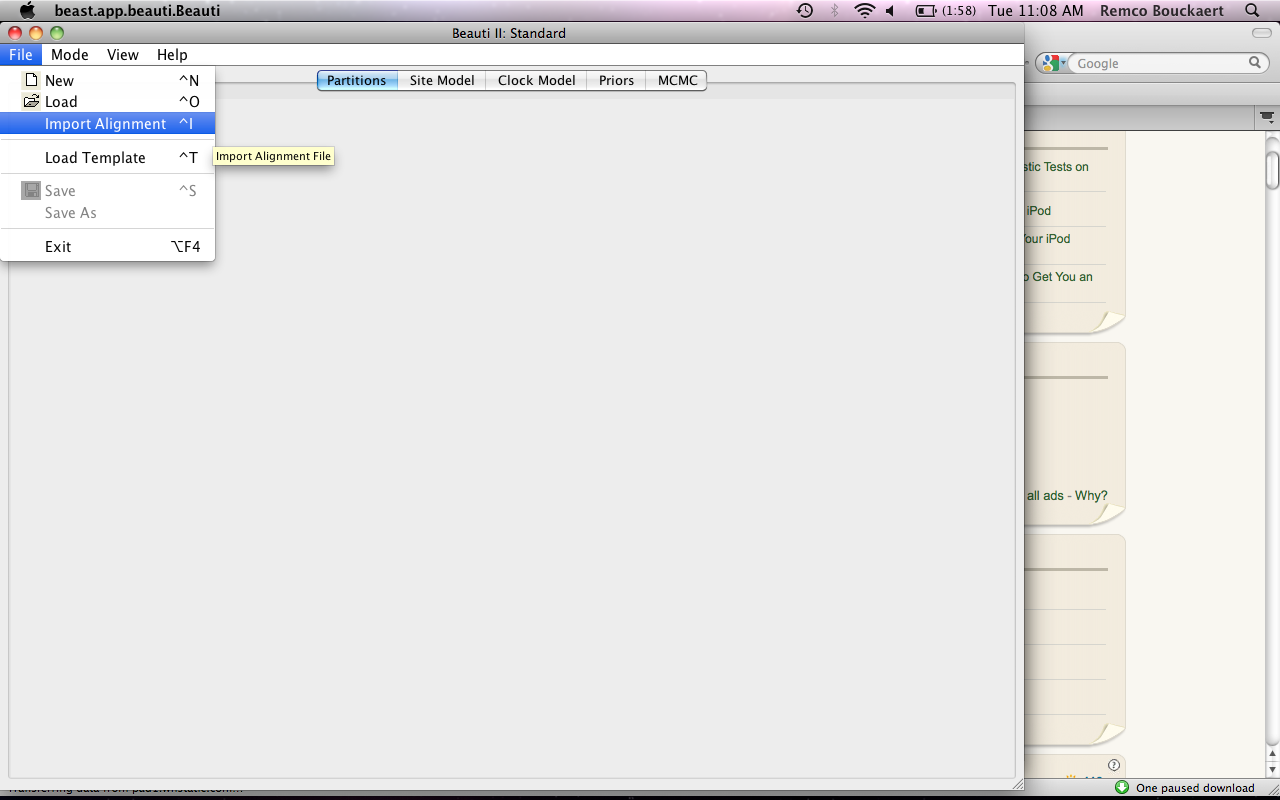
\includegraphics[width=\textwidth]{figures/ImportNexus}
%
%\caption{A screenshot of the import nexus file menu option in BEAUti. \TODO{Need to have the correct menu shortcuts for OS X!}}
%\label{fig:BEAUti_ImportNexus}
%\end{figure}

The example file called \texttt{primates-mtDNA.nex} is in the {\tt examples/nexus/} directory of the directory where BEAST was installed.
This file contains an alignment of sequences of 12 species of primates. 
%It looks likethis (the lines have been truncated):
%
%\begin{verbatim}
%#NEXUS
%begin data;
%dimensions ntax=12 nchar=898;
%format datatype=dna interleave=no gap=-;
%matrix
%Tarsius_syrichta  AAGTTTCATTGGAGCCACCACTCTTATAATTGCCCATGGCCTCACC
%Lemur_catta       AAGCTTCATAGGAGCAACCATTCTAATAATCGCACATGGCCTTACA
%Homo_sapiens	     AAGCTTCACCGGCGCAGTCATTCTCATAATCGCCCACGGGCTTACA
%Pan               AAGCTTCACCGGCGCAATTATCCTCATAATCGCCCACGGACTTACA
%Gorilla           AAGCTTCACCGGCGCAGTTGTTCTTATAATTGCCCACGGACTTACA
%Pongo             AAGCTTCACCGGCGCAACCACCCTCATGATTGCCCATGGACTCACA
%Hylobates         AAGCTTTACAGGTGCAACCGTCCTCATAATCGCCCACGGACTAACC
%Macaca_fuscata    AAGCTTTTCCGGCGCAACCATCCTTATGATCGCTCACGGACTCACC
%M_mulatta         AAGCTTTTCTGGCGCAACCATCCTCATGATTGCTCACGGACTCACC
%M_fascicularis    AAGCTTCTCCGGCGCAACCACCCTTATAATCGCCCACGGGCTCACC
%M_sylvanus        AAGCTTCTCCGGTGCAACTATCCTTATAGTTGCCCATGGACTCACC
%Saimiri_sciureus	 AAGCTTCACCGGCGCAATGATCCTAATAATCGCTCACGGGTTTACT
%;
%end;
%
%begin assumptions;
%	charset firsthalf = 1-449;
%	charset secondhalf = 450-898;
%end;
%end;\end{verbatim}
%
%\medskip{}

Once loaded, five character partitions are displayed in the main panel (Figure \ref{fig:BEAUTI_DataPartitions}). {\bf You must remove the `coding' partition before continuing to the next step as it refers to the same nucleotides as partitions `1stpos', `2ndpos' and `3rdpos'.} To remove the `coding' partition select the row and click the `-' button at the bottom of the table. 
%You can view the alignment by double clicking the partition (Figure \ref{fig:BEAUTI_AlignmentViewer}).

\begin{figure}

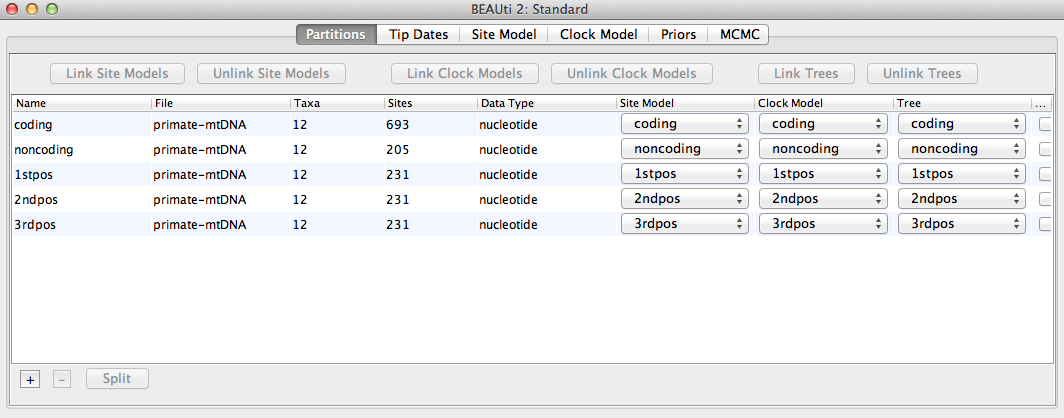
\includegraphics[width=\textwidth]{figures/BEAUti_DataPartitions}
\caption{A screenshot of the data tab in BEAUti.}
\label{fig:BEAUTI_DataPartitions}
\end{figure}

%\begin{figure}[h]
%
%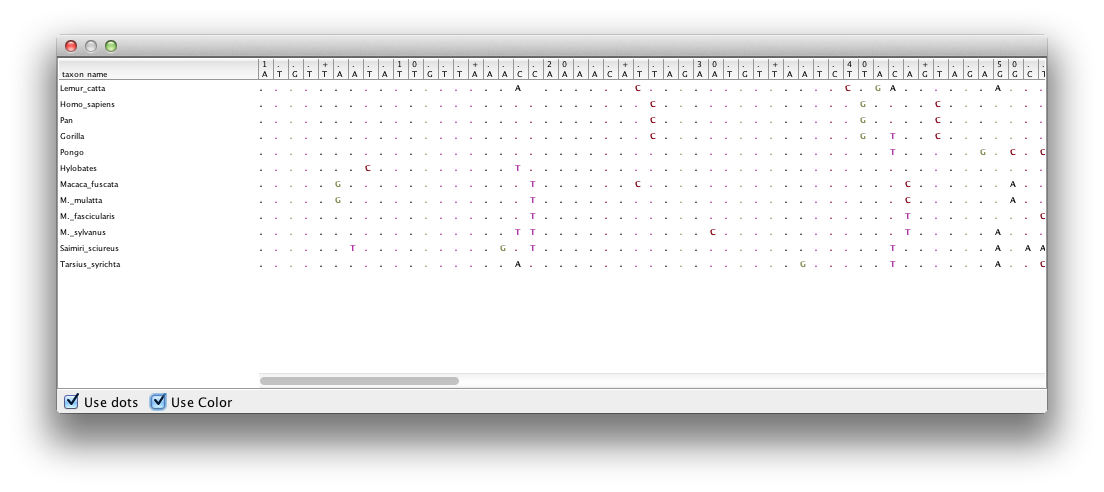
\includegraphics[width=\textwidth]{figures/AlignmentViewer}
%
%\caption{A screenshot of the alignment viewer in BEAUti.}
%\label{fig:BEAUTI_AlignmentViewer}
%\end{figure}

\subsection*{Link/Unlink partition models}

At this point we will need to link the clock model and tree. In the {\bf Partitions} panel, select all four partitions in the table (or none, by default all partitions are affected) and click the \texttt{Link Tree Models} button and then the \texttt{Link Clock Models} button (see Figure \ref{fig:BEAUti_DataPartitions_final}). Then click on the first drop-down menu in the Clock Model column and rename the shared clock model to `clock'. Likewise rename the shared tree to `tree'. This will make following options and generated log files more easy to read.

\begin{figure}

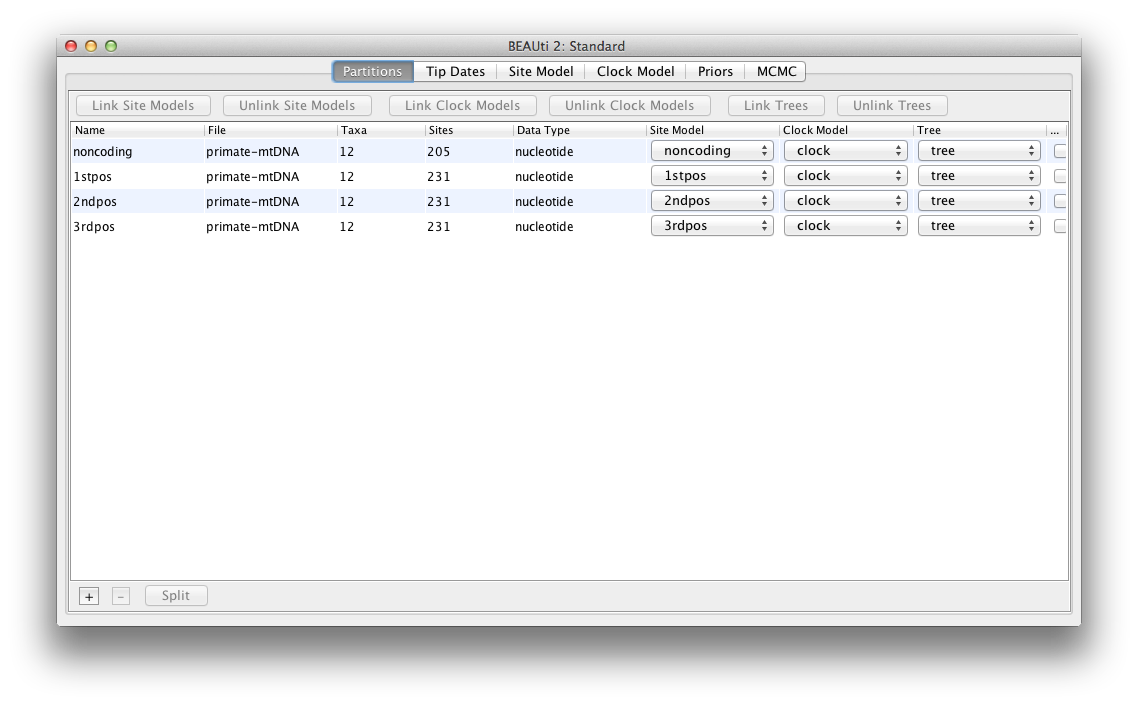
\includegraphics[width=\textwidth]{figures/BEAUti_DataPartitions_final}
\caption{A screenshot of the Partitions tab in BEAUti after linking and renaming the clock model and tree.}
\label{fig:BEAUti_DataPartitions_final}
\end{figure}

\subsection{Setting the substitution model}

The next step is to set up the substitution model. First we will temporarily link the site models in the Partitions panel so that we can change the model of all partitions simultaneously. Then, select the {\bf Site Models} tab at the top of the
main window. This will reveal the evolutionary model settings for
BEAST. The options available depend on whether the data are
nucleotides, or amino acids, binary data, or general data.
The settings that will appear after loading the primate nucleotide alignment will
be the default values for nucleotide data so we need to make some changes. 

Most of the models should be familiar to you. %(see Chapter {\ref{chapter:SubstitutionModels} for details}). 
First, set the \textbf{Gamma Category Count} to 4 and then check the `estimate' box for the \textbf{Shape} parameter. This will allow rate variation 
between sites in each partition to be modeled.  Then select  \textbf{HKY} from the \textbf{Subst Model} drop-down menu (Figure \ref{fig:BEAUti_Model}) and select \textbf{Empirical} from the \textbf{Frequencies} drop-down menu. This will fix the frequencies to the proportions observed in the data (for each partition individually, once we unlink the site models again). This approach means that we can get a good fit to the data without explicitly estimating these parameters. We do it here simply to make the log files a bit shorter and more readable in later parts of the exercise. Finally check the `estimate' box for the \textbf{Mutation rate} parameter and select the \textbf{Fix mean mutation rate} check box. This will allow the individual partitions to have their relative rates estimated once we unlink the site models.

\begin{figure}
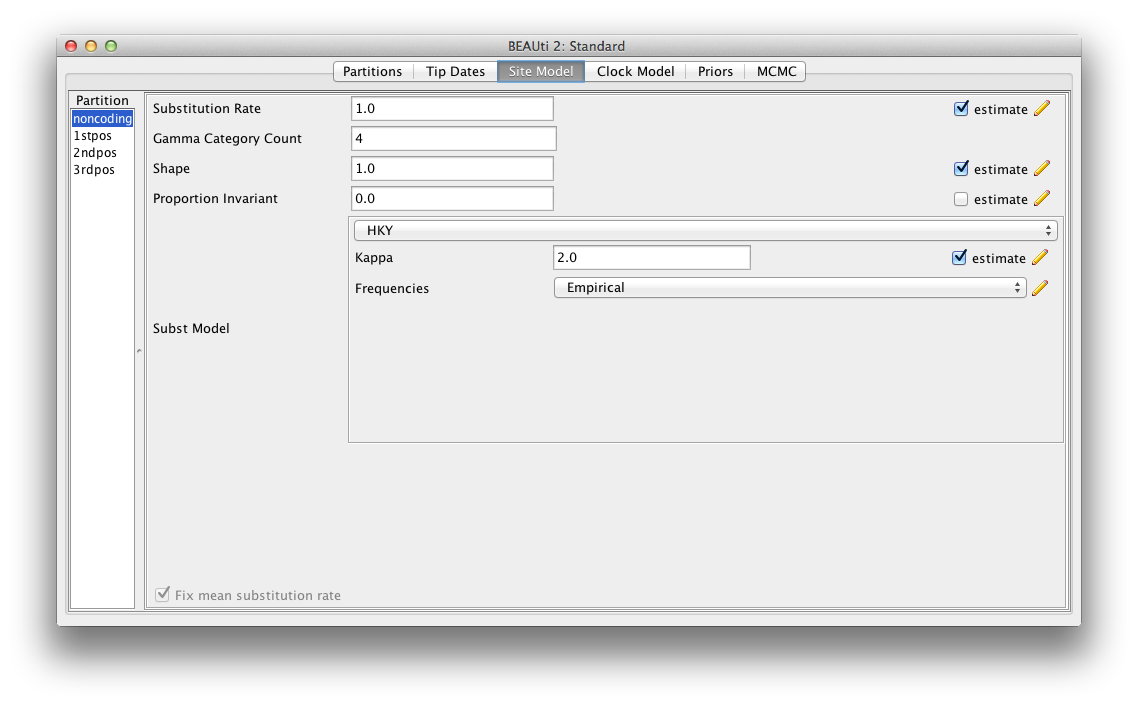
\includegraphics[width=\textwidth]{figures/BEAUti_Model}
\caption{A screenshot of the site model tab in BEAUti.}
\label{fig:BEAUti_Model}
\end{figure}

Now, return to the `Partitions' panel and unlink the site models so that each partition has its own named site model with independent substitution model parameters and relative rate.
%Finally, in order to allow for a different absolute rate of evolution for each partition we will return to the `Site Model' panel and check `estimate' for the \textbf{Mutation Rate} for each of partitions \textbf{noncoding}, \textbf{1stpos}, \textbf{2ndpos} in turn. Don't check `estimate' for the \textpos{3rdpos} because this is the rate that the other partitions will be estimated relative to.

\subsection{Setting the clock model}

The next step is to select the {\bf Clock Models} tab at the top of the
main window. This is where we select the molecular clock model. For this exercise we are going to leave the selection at the {\it default} value of a Strict molecular clock, because this data is very clock-like and does not need rate variation among branches to be included in the model.

%\begin{figure}
%\includegraphics[width=\textwidth]{figures/BEAUti_Clock}
%\caption{A screenshot of the clock model tab in BEAUti.}
%\label{fig:BEAUti_Clock}
%\end{figure}

\subsection{Priors }

The {\bf Priors} tab allows priors to be specified for each parameter in the
model. The model selections made in the site model and clock model tabs, result in the inclusion of various parameters
in the model, and these are shown in the priors tab (see Figure \ref{fig:BEAUti_Prior1}).

\begin{figure}
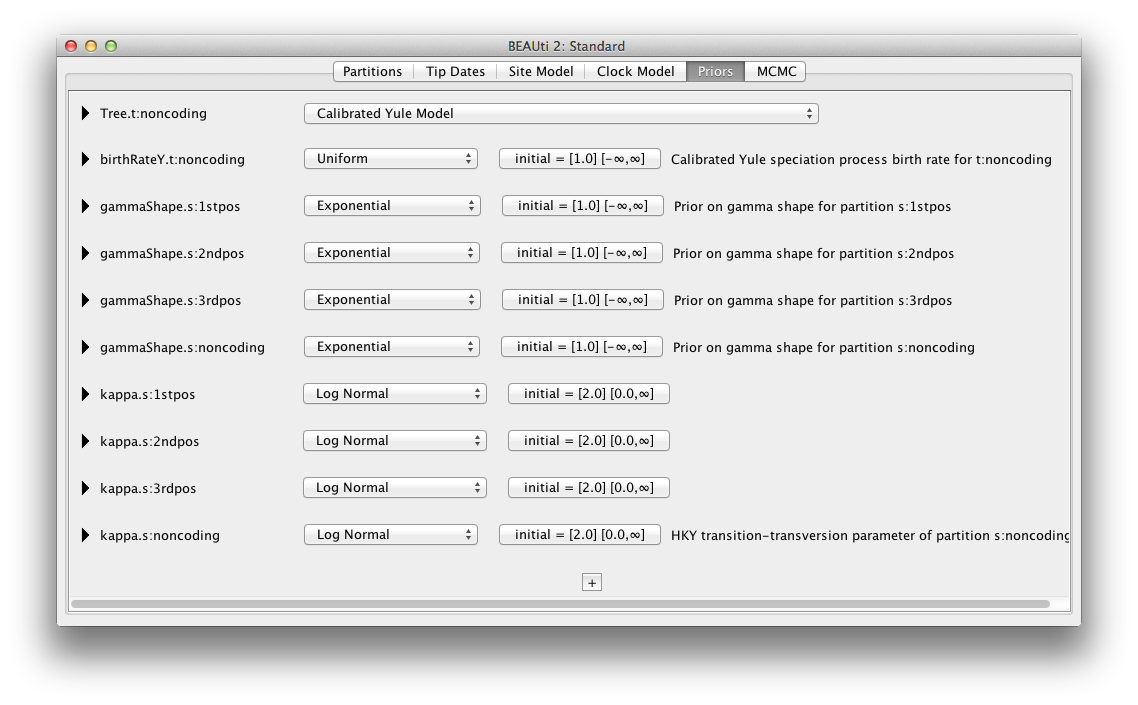
\includegraphics[width=\textwidth]{figures/BEAUti_Prior1}
\caption{A screenshot of the Priors tab in BEAUti. }
\label{fig:BEAUti_Prior1}
\end{figure}

Here we also specify that we wish to use the Calibrated Yule model \cite{Heled:2012fk}
as the tree prior. This is a simple model of speciation that
is generally more appropriate when considering sequences from different species %(see Section \ref{section:YuleBirthDeathModels} for details).
Select this from the {\bf Tree prior} dropdown menu.

%\begin{figure}
%\includegraphics[width=\textwidth]{figures/BEAUti_Tree}
%\caption{A screenshot of the tree prior drop down menu in BEAUti.}
%\label{fig:BEAUti_Tree}
%\end{figure}

\subsubsection{Defining the calibration node}

To define an extra prior, press the small {\bf +} button below list of priors. You will see a
dialog that allows you to define a subset of the taxa in the phylogenetic tree. Once you have created a taxa set you will be able to add calibration information for its most recent common
ancestor (MRCA) later on. 

Name the taxa set by filling in the taxon set label entry. 
Call it \texttt{human-chimp} (it will contain the taxa for {\it Homo sapiens} and {\it Pan}).
In next list below you will see the available taxa. Select each of the two taxa in turn and press the $> >$ arrow button. 
Click OK and the newly defined taxa set will be added in to the prior list.
As this is a calibrated node to be used in conjunction with the Calibrated Yule prior, monophyly must be enforced, so select the checkbox marked \texttt{Monophyletic?}. This will constrain the tree topology so that the human-chimp grouping is kept monophyletic during the course of the MCMC analysis.

We now need to specify a prior distribution on the calibrated node, based on our prior fossil knowledge. This is known
as calibrating our tree. Select the \textbf{Normal} distribution from the drop down menu to the right of the newly added \texttt{human-chimp.prior}. Click on the black triangle to the right and
a graph of the probability density function will appear, along with parameters for the normal distribution.
We are going to specify a normal distribution centered at 6 million
years with a standard deviation of 0.5 million years. This will give
a central 95\% range of about 5-7 My. This roughly corresponds to the current consensus
estimate of the date of the most recent common ancestor of humans and chimpanzees (Figure \ref{fig:BEAUti_TaxonSets}).

\begin{figure}
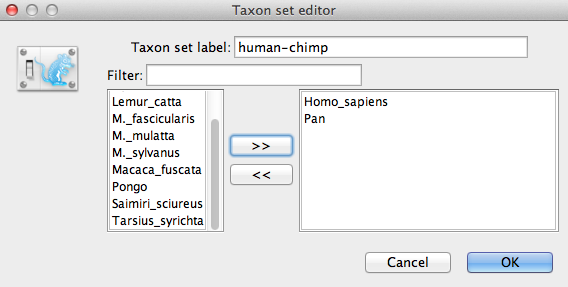
\includegraphics[width=\textwidth]{figures/BEAUti_TaxonSets}
\caption{A screenshot of the calibration prior options in the Priors panel in BEAUti.}
\label{fig:BEAUti_TaxonSets}
\end{figure}

Finally we will also specify some diffuse ``uninformative'' but proper priors on the overall molecular clock rate (\texttt{clockRate}) and the speciation rate (\texttt{birthRateY}) of the Yule tree prior. For each of these parameters select \textbf{Gamma} from the drop-down menu and using the arrow button to the right, expand the view to reveal the parameters of the Gamma prior. For both the clock rate and the Yule birth rate set the Alpha (shape) parameter to 0.001 and the Beta (scale) parameter to 1000.


%Finally, put a log-normal distribution on the kappa parameters. \TODO{with what M and S parameters?}
%The clock model parameters will appear when the clock rate is estimated. 
%The priors table should now look like Figure \ref{fig:BEAUti_Prior2}.

%\begin{figure}
%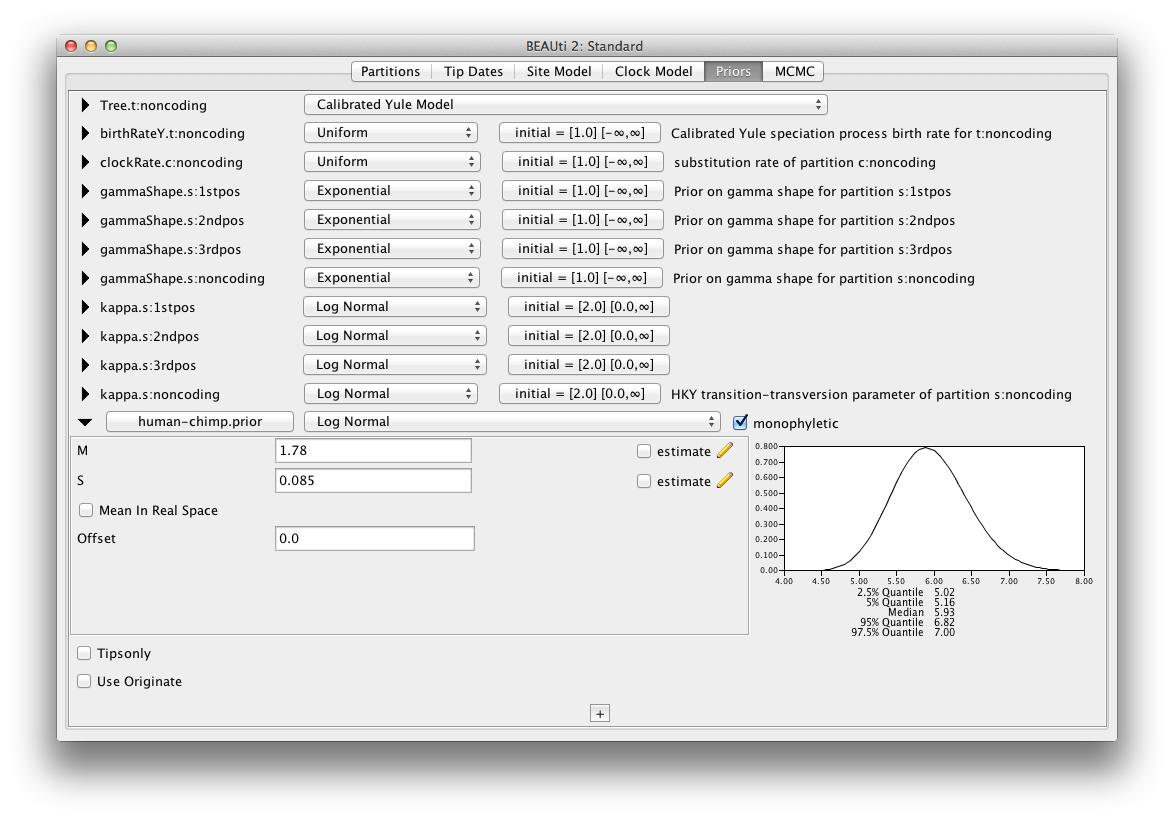
\includegraphics[width=\textwidth]{figures/BEAUti_Prior2}
%\caption{A screenshot of the newly added calibration prior in the Priors panel in BEAUti. \TODO{This figure needs to be changed to remove the HomiCerco.prior.}}
%\label{fig:BEAUti_Prior2}
%\end{figure}

\subsection{Setting the MCMC options}

%Ignore the \textbf{Operators} tab as this just contains technical
%settings affecting the efficiency of the MCMC program (see Notes for details). 

The next tab, {\bf MCMC}, provides more general
settings to control the length of the MCMC run and the file names. 

Firstly we have the \textbf{Chain Length}. This is the number of
steps the MCMC will make in the chain before finishing. How long this
should be depends on the size of the data set, the complexity of the
model and the quality of answer required. The default value of 10,000,000
is entirely arbitrary and should be adjusted according to the size
of your data set. For this data set let's initially set the chain
length to \chainLength{} as this will run reasonably quickly on most modern
computers (a few minutes).

%\begin{figure}
%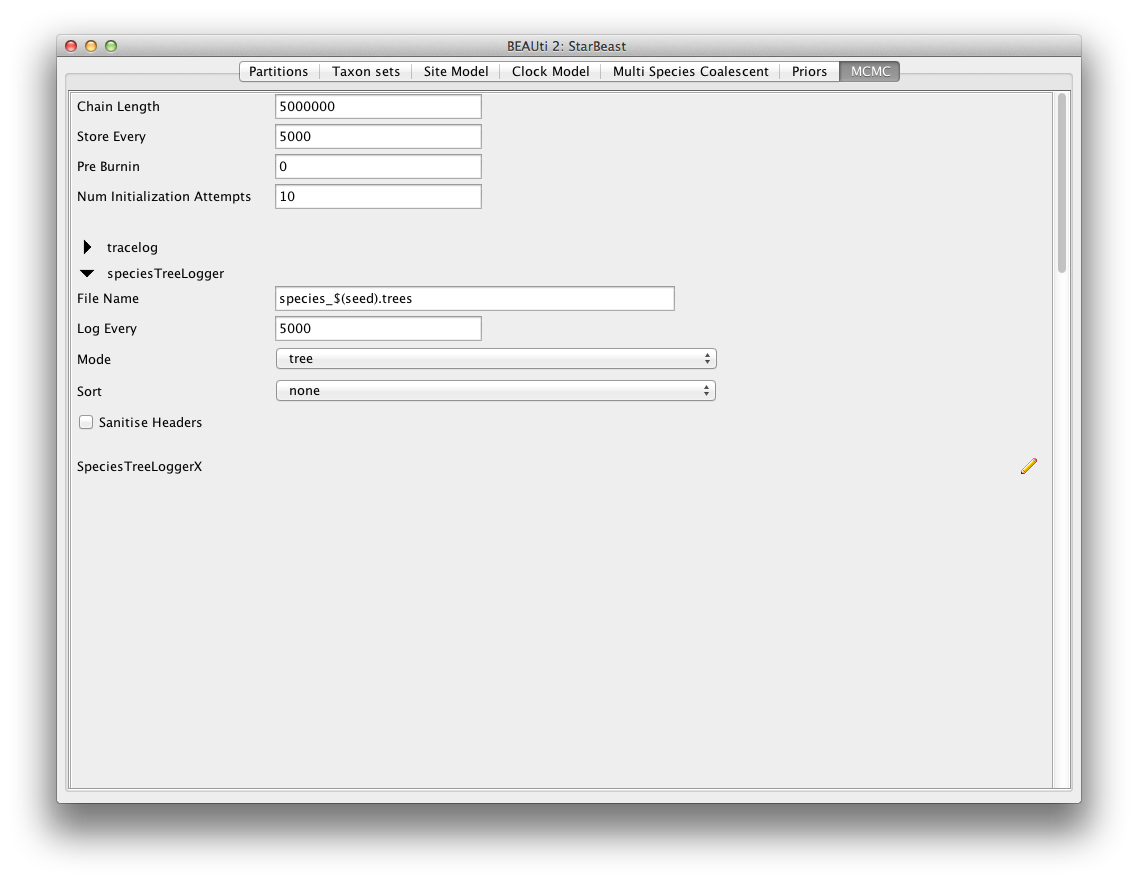
\includegraphics[width=\textwidth]{figures/BEAUti_MCMC}
%\caption{A screenshot of the MCMC panel in BEAUti.}
%\label{fig:BEAUti_MCMC}
%\end{figure}

We will leave the \textbf{Store Every}  and \textbf{Pre Burnin} fields set to their default values. Below these are the details of the log files. Each one can be expanded by clicking the arrow to the right

The next options specify how often the parameter values in the Markov
chain should be displayed on the screen and recorded in the log file.
The screen output is simply for monitoring the programs progress so
can be set to any value (although if set too small, the sheer quantity
of information being displayed on the screen will actually slow the
program down). For the log file, the value should be set relative
to the total length of the chain. Sampling too often will result in
very large files with little extra benefit in terms of the accuracy
of the analysis. Sample too infrequently and the log file will not
record sufficient information about the distributions of the parameters. 
You probably want to aim to store no more than 10,000 samples so this should be
set to no less than chain length / 10000.

For this exercise we will set the screen log to \screenEvery{} and the file log to \logEvery{}. The final two
options give the file names of the log files for the sampled parameters and
the trees. These will be set to a default based on the name of the
imported NEXUS file. 

\begin{itemize}
\item If you are using the Windows operating system then we suggest you add the suffix \texttt{.txt} to both of these (so,
\texttt{Primates.log.txt} and \texttt{Primates.trees.txt}) so that Windows recognizes
these as text files. 
\end{itemize}

\subsection{Generating the BEAST XML file }

We are now ready to create the BEAST XML file. To do this,
select the \textbf{Save} option from the \textbf{File} menu. 
Check the default priors, and save the file with an appropriate name
(we usually end the filename with \texttt{.xml}, i.e., \texttt{Primates.xml}).
We are now ready to run the file through BEAST. 

\section{Running BEAST }

\begin{figure}
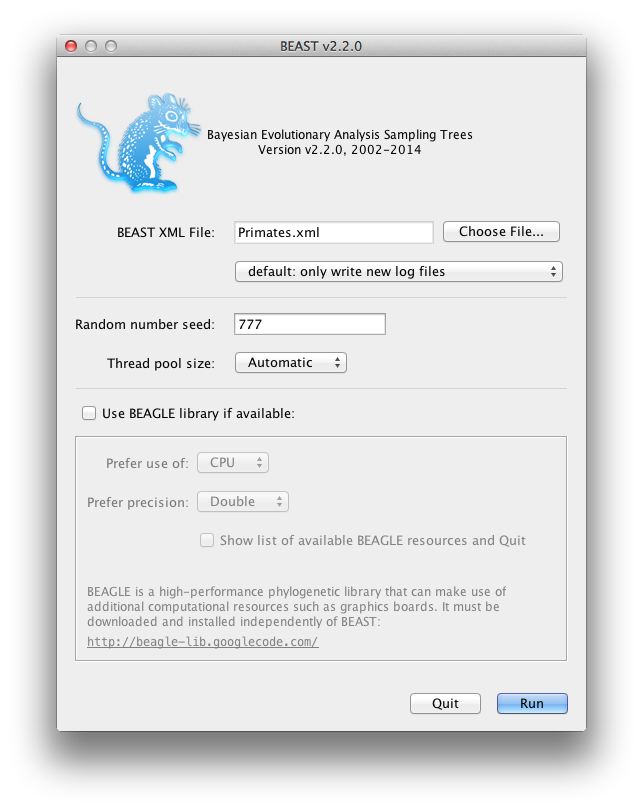
\includegraphics[width=\textwidth]{figures/BEAST}
\caption{A screenshot of BEAST.}
\label{fig:BEAST}
\end{figure}

Now run BEAST and when it asks for an input file, provide your newly
created XML file as input. BEAST will then run until it has finished
reporting information to the screen. The actual results files are
save to the disk in the same location as your input file. The output to the screen will
look something like this: 

{\scriptsize   
\begin{verbatim}
          BEAST v2.0.d Prerelease r613, 2002-2011
       Bayesian Evolutionary Analysis Sampling Trees
                 Designed and developed by
Remco Bouckaert, Alexei J. Drummond, Andrew Rambaut and Marc A. Suchard
                              
               Department of Computer Science
                   University of Auckland
                  remco@cs.auckland.ac.nz
                  alexei@cs.auckland.ac.nz
                              
             Institute of Evolutionary Biology
                  University of Edinburgh
                     a.rambaut@ed.ac.uk
                              
              David Geffen School of Medicine
           University of California, Los Angeles
                     msuchard@ucla.edu
                              
                Downloads, Help & Resources:
              	http://beast2.cs.auckland.ac.nz
                              
Source code distributed under the GNU Lesser General Public License:
              	http://code.google.com/p/beast2
                              
                     BEAST developers:
	Alex Alekseyenko, Trevor Bedford, Erik Bloomquist, Joseph Heled, 
	Sebastian Hoehna, Denise Kuehnert, Philippe Lemey, Wai Lok Sibon Li, 
	Gerton Lunter, Sidney Markowitz, Vladimir Minin, Michael Defoin Platel, 
          	Oliver Pybus, Chieh-Hsi Wu, Walter Xie
                              
                         Thanks to:
    	Roald Forsberg, Beth Shapiro and Korbinian Strimmer


Random number seed: 777

12 taxa
898 sites
413 patterns
TreeLikelihood uses beast.evolution.likelihood.BeerLikelihoodCore4
TreeLikelihood uses beast.evolution.likelihood.BeerLikelihoodCore4
TreeLikelihood uses beast.evolution.likelihood.BeerLikelihoodCore4
TreeLikelihood uses beast.evolution.likelihood.BeerLikelihoodCore4
======================================================
Please cite the following when publishing this model:

A prototype for BEAST 2.0: The computational science of evolutionary software. Bouckaert, Drummond, Rambaut, Alekseyenko, Suchard, Walter & the BEAST Core Development Team. 2010

Heled J, Drummond AJ. Calibrated Tree Priors for Relaxed Phylogenetics and Divergence Time Estimation. Syst Biol (2012) 61 (1): 138-149.

Hasegawa, M., Kishino, H and Yano, T. 1985. Dating the human-ape splitting by a molecular clock of mitochondrial DNA. Journal of Molecular Evolution 22:160-174.


======================================================
Trying to write file primate-mtDNA.777.log but the file already exists (perhaps use the -overwrite flag?).
Overwrite (Y/N)?:
Y
Writing file primate-mtDNA.777.log
         Sample      posterior ESS(posterior)     likelihood          prior
Writing file primate-mtDNA.tree.777.trees
              0     -7766.9711              N     -7688.4922       -78.4789 --
          10000     -5527.1265         2.0        -5453.0299       -74.0966 --
          20000     -5521.2666         3.0        -5446.4954       -74.7711 --
          30000     -5518.7901         4.0        -5442.6380       -76.1520 --
          40000     -5514.6676         5.0        -5438.3693       -76.2982 --
          50000     -5522.7987         6.0        -5447.3333       -75.4654 --
          60000     -5513.6936         7.0        -5440.6748       -73.0187 2m50s/Msamples
          ...
        9990000     -5512.1732       739.1        -5441.1958       -70.9773 2m49s/Msamples
       10000000     -5515.2321       734.5        -5437.9182       -77.3138 2m49s/Msamples
Operator                                                              Tuning	#accept	#reject	#total	acceptance rate
ScaleOperator_treeScaler.t:tree                                       0.728 	75940	281958	357898	0.212 
ScaleOperator_treeRootScaler.t:tree                                   0.581 	48659	309158	357817	0.136 
Uniform_UniformOperator.t:tree                                              	799104	2781229	3580333	0.223 
SubtreeSlide_SubtreeSlide.t:tree                                      10.01 	450154	1339576	1789730	0.252 
Exchange_narrow.t:tree                                                      	1368	1787165	1788533	0.001 
Exchange_wide.t:tree                                                        	25	357913	357938	0 
WilsonBalding_WilsonBalding.t:tree                                          	14	358742	358756	0 
ScaleOperator_gammaShapeScaler.s:noncoding                            0.369 	2843	8998	11841	0.24 
ScaleOperator_KappaScaler.s:noncoding                                 0.352 	2950	8870	11820	0.25 
DeltaExchangeOperator_FixMeanMutationRatesOperator                    0.340 	35796	203561	239357	0.15 
ScaleOperator_KappaScaler.s:1stpos                                    0.420 	2713	9297	12010	0.226 
ScaleOperator_gammaShapeScaler.s:1stpos                               0.419 	3266	8762	12028	0.272 
ScaleOperator_KappaScaler.s:2ndpos                                    0.324 	2886	8933	11819	0.244 
ScaleOperator_gammaShapeScaler.s:2ndpos                               0.278 	2984	9046	12030	0.248 
ScaleOperator_KappaScaler.s:3rdpos                                    0.541 	2622	9246	11868	0.221 
ScaleOperator_gammaShapeScaler.s:3rdpos                               0.308 	3343	8577	11920	0.28 
ScaleOperator_CalibratedYuleBirthRateScaler.t:tree                    0.249 	98194	258404	356598	0.275 
ScaleOperator_StrictClockRateScaler.c:clock                           0.704 	82888	276401	359289	0.231 
UpDownOperator_strictClockUpDownOperator.c:clock                      0.600 	85379	273037	358416	0.238 
Total calculation time: 1710.509 seconds
\end{verbatim}}

\section{Analyzing the results}

Run the program called {\bf Tracer} to analyze the output of BEAST. When the main
window has opened, choose {\bf Import Trace File...} from the {\bf File} menu and select the file that
BEAST has created called \texttt{Primates.log} (Figure \ref{fig:Tracer1}).

\begin{figure}
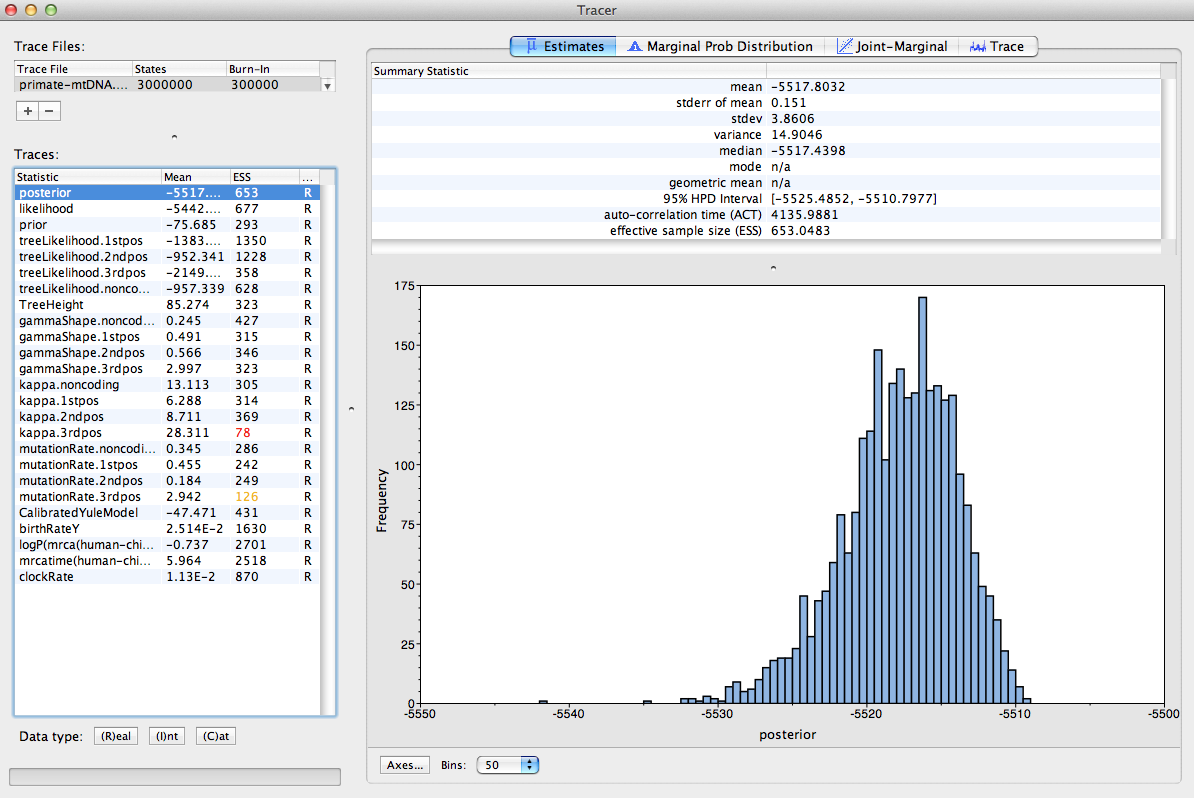
\includegraphics[width=\textwidth]{figures/Tracer1}
\caption{A screenshot of Tracer v{\TracerVersion}.}
\label{fig:Tracer1}
\end{figure}

Remember that MCMC is a stochastic algorithm so the actual numbers will not be exactly the same as those depicted in the figure.

On the left hand side is a list of the different quantities that BEAST has logged to file. 
There are traces for the posterior (this
is the natural logarithm of the product of the tree likelihood and the prior density), and the continuous parameters. Selecting a trace
on the left brings up analyses for this trace on the right hand side depending on tab that is selected. When first opened, the
`posterior' trace is selected and various statistics of this trace are shown under the Estimates tab.
In the top right of the window is a table of calculated statistics for the selected trace. 

Select the \texttt{clockRate} parameter in the lefthand list to look at
the average rate of evolution (averaged over the whole tree and all sites). Tracer will plot a (marginal posterior) histogram for the selected statistic and also give you
summary statistics such as the mean and median. The 95\% HPD stands for {\it highest posterior density interval} and represents the most compact interval on the selected parameter that contains 95\% of the posterior probability. It can be loosely thought of as a Bayesian analog to a confidence interval. The \texttt{TreeHeight} parameter gives the marginal posterior distribution of the age of the root of the entire tree.

Select the \texttt{TreeHeight} parameter and then Ctrl-click \texttt{mrcatime(human-chimp)}  (Command-click on Mac OS X). This will show a display of the
age of the root and the calibration MRCA we specified earlier in BEAUti. You can verify that the divergence that we used to calibrate the tree
(\texttt{mrcatime(human-chimp)}) has a posterior distribution that matches the prior distribution we specified (Figure \ref{fig:Tracer_divergences}).

\begin{figure}
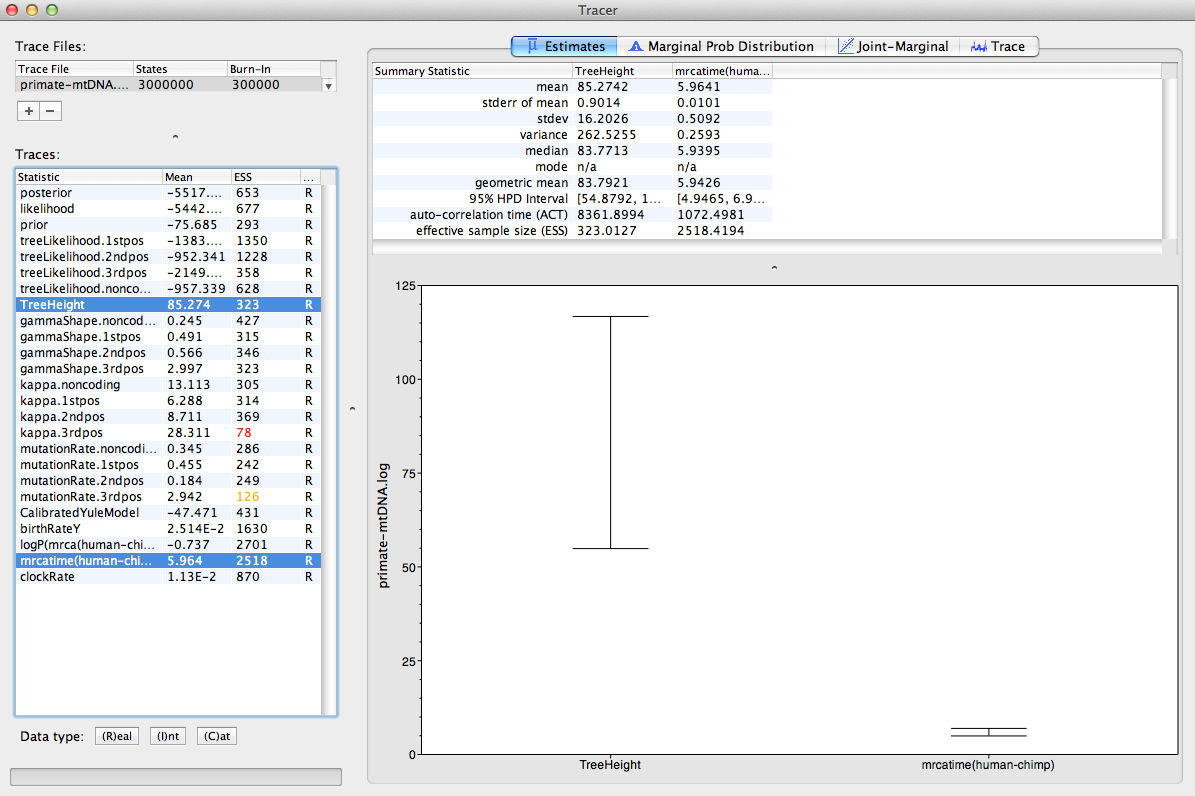
\includegraphics[width=\textwidth]{figures/Tracer_divergences}
\caption{A screenshot of the 95\% HPD intervals of the root height and the user-specified (human-chimp) MRCA in Tracer.}
\label{fig:Tracer_divergences}
\end{figure}

\begin{figure}
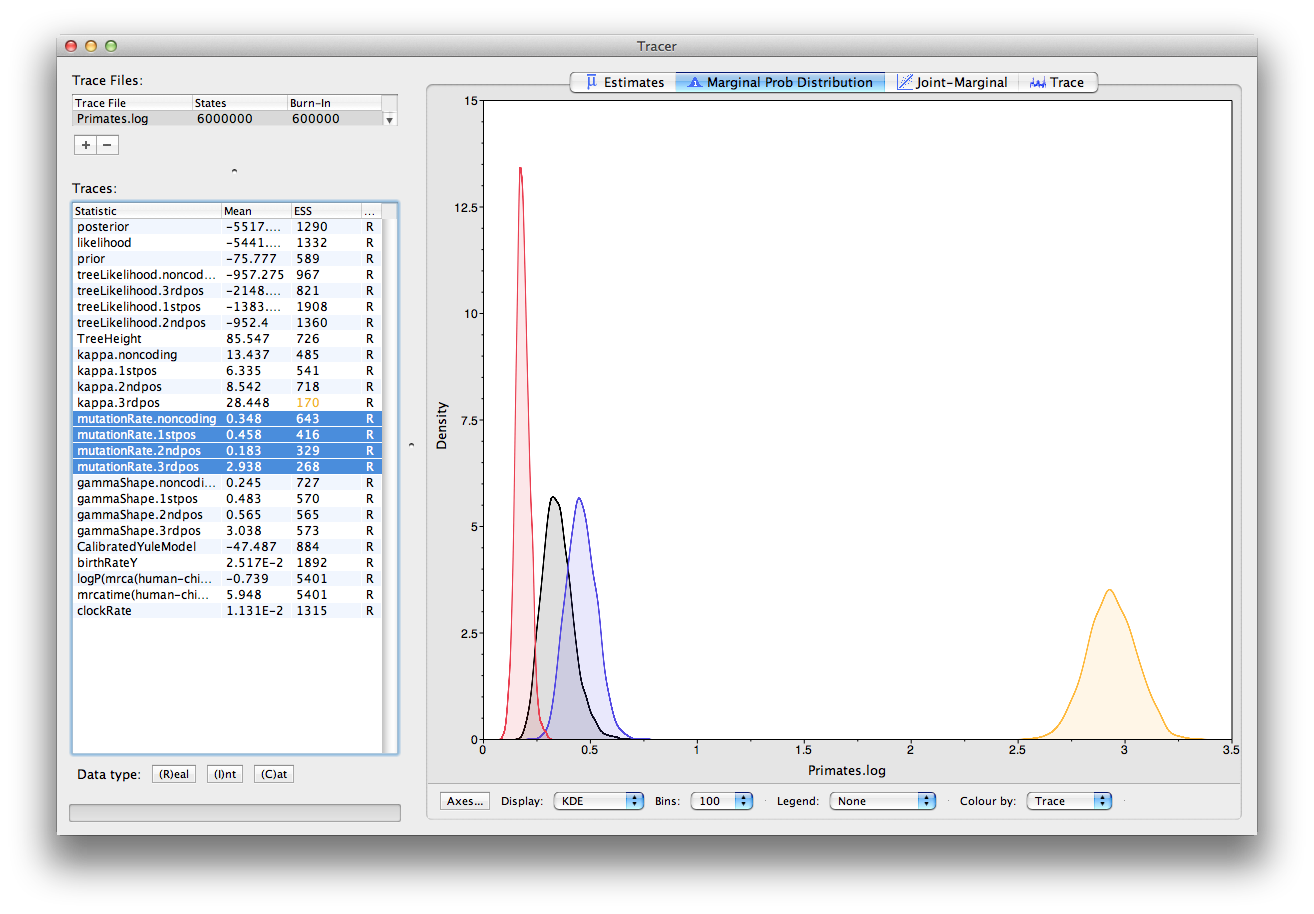
\includegraphics[width=\textwidth]{figures/Tracer_marginalDensity}
\caption{A screenshot of the marginal posterior densities of the relative substitution rates of the four partitions (relative to the site-weighted mean rate). This plot shows that codon positions 1 and 2 have substantially different rates (0.452 versus 0.181) and both are far slower than codon position 3 with a relative rate of 2.95. The noncoding partition has a rate intermediate between codon positions 1 and 2 (0.344). Taken together this result suggests strong purifying selection in both the coding and noncoding regions of the alignment.}
\label{fig:Tracer_marginalDensity}
\end{figure}


\if0
\begin{figure}

% Created by tikzDevice version 0.6.2 on 2014-09-24 13:25:09
% !TEX encoding = UTF-8 Unicode
\documentclass[margin=1pt]{standalone}
\usepackage{tikz}
\begin{document}

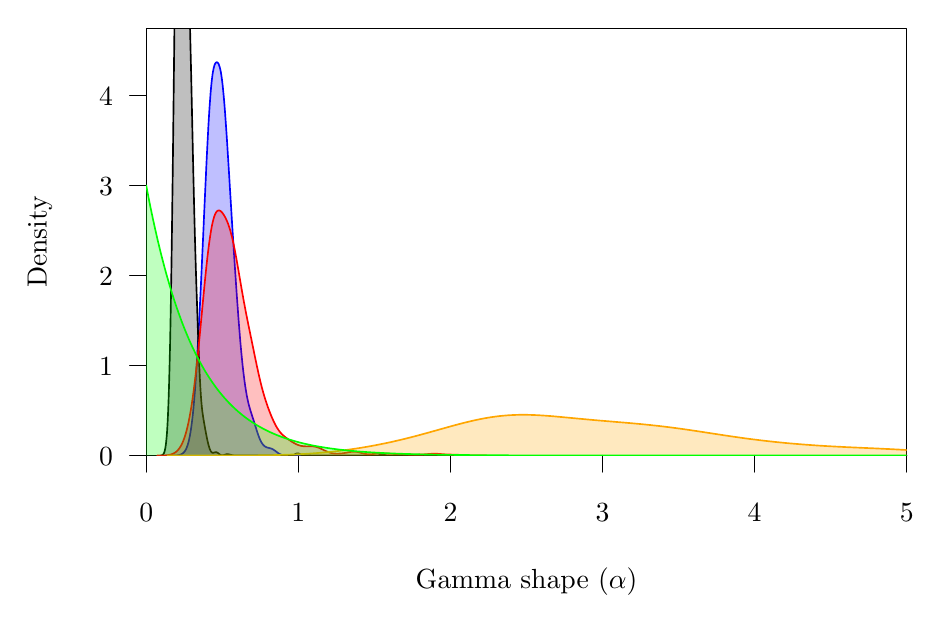
\begin{tikzpicture}[x=1pt,y=1pt]
\definecolor[named]{drawColor}{rgb}{0.00,0.00,0.00}
\definecolor[named]{fillColor}{rgb}{1.00,1.00,1.00}
%\fill[color=fillColor,fill opacity=0.00,] (0,0) rectangle (325.21,216.81);
\begin{scope}
%\path[clip] (  0.00,  0.00) rectangle (325.21,216.81);
\definecolor[named]{drawColor}{rgb}{0.00,0.00,0.00}

\draw[color=drawColor,line cap=round,line join=round,fill opacity=0.00,] ( 49.20, 49.20) -- (324.02, 49.20);

\draw[color=drawColor,line cap=round,line join=round,fill opacity=0.00,] ( 49.20, 49.20) -- ( 49.20, 43.20);

\draw[color=drawColor,line cap=round,line join=round,fill opacity=0.00,] (104.16, 49.20) -- (104.16, 43.20);

\draw[color=drawColor,line cap=round,line join=round,fill opacity=0.00,] (159.13, 49.20) -- (159.13, 43.20);

\draw[color=drawColor,line cap=round,line join=round,fill opacity=0.00,] (214.09, 49.20) -- (214.09, 43.20);

\draw[color=drawColor,line cap=round,line join=round,fill opacity=0.00,] (269.05, 49.20) -- (269.05, 43.20);

\draw[color=drawColor,line cap=round,line join=round,fill opacity=0.00,] (324.02, 49.20) -- (324.02, 43.20);

\node[color=drawColor,anchor=base,inner sep=0pt, outer sep=0pt, scale=  1.00] at ( 49.20, 25.20) {0};

\node[color=drawColor,anchor=base,inner sep=0pt, outer sep=0pt, scale=  1.00] at (104.16, 25.20) {1};

\node[color=drawColor,anchor=base,inner sep=0pt, outer sep=0pt, scale=  1.00] at (159.13, 25.20) {2};

\node[color=drawColor,anchor=base,inner sep=0pt, outer sep=0pt, scale=  1.00] at (214.09, 25.20) {3};

\node[color=drawColor,anchor=base,inner sep=0pt, outer sep=0pt, scale=  1.00] at (269.05, 25.20) {4};

\node[color=drawColor,anchor=base,inner sep=0pt, outer sep=0pt, scale=  1.00] at (324.02, 25.20) {5};

\draw[color=drawColor,line cap=round,line join=round,fill opacity=0.00,] ( 49.20, 49.20) -- ( 49.20,179.23);

\draw[color=drawColor,line cap=round,line join=round,fill opacity=0.00,] ( 49.20, 49.20) -- ( 43.20, 49.20);

\draw[color=drawColor,line cap=round,line join=round,fill opacity=0.00,] ( 49.20, 81.71) -- ( 43.20, 81.71);

\draw[color=drawColor,line cap=round,line join=round,fill opacity=0.00,] ( 49.20,114.21) -- ( 43.20,114.21);

\draw[color=drawColor,line cap=round,line join=round,fill opacity=0.00,] ( 49.20,146.72) -- ( 43.20,146.72);

\draw[color=drawColor,line cap=round,line join=round,fill opacity=0.00,] ( 49.20,179.23) -- ( 43.20,179.23);

\node[color=drawColor,anchor=base east,inner sep=0pt, outer sep=0pt, scale=  1.00] at ( 37.20, 45.76) {0};

\node[color=drawColor,anchor=base east,inner sep=0pt, outer sep=0pt, scale=  1.00] at ( 37.20, 78.26) {1};

\node[color=drawColor,anchor=base east,inner sep=0pt, outer sep=0pt, scale=  1.00] at ( 37.20,110.77) {2};

\node[color=drawColor,anchor=base east,inner sep=0pt, outer sep=0pt, scale=  1.00] at ( 37.20,143.28) {3};

\node[color=drawColor,anchor=base east,inner sep=0pt, outer sep=0pt, scale=  1.00] at ( 37.20,175.79) {4};

\draw[color=drawColor,line cap=round,line join=round,fill opacity=0.00,] ( 49.20, 49.20) --
	(324.01, 49.20) --
	(324.01,203.61) --
	( 49.20,203.61) --
	( 49.20, 49.20);
\end{scope}
\begin{scope}
%\path[clip] (  0.00,  0.00) rectangle (325.21,216.81);
\definecolor[named]{drawColor}{rgb}{0.00,0.00,0.00}

\node[color=drawColor,anchor=base,inner sep=0pt, outer sep=0pt, scale=  1.00] at (186.61,  1.20) {Gamma shape ($\alpha$)};

\node[rotate= 90.00,color=drawColor,anchor=base,inner sep=0pt, outer sep=0pt, scale=  1.00] at ( 13.20,126.41) {Density};
\end{scope}
\begin{scope}
\path[clip] ( 49.20, 49.20) rectangle (324.01,203.61);
\definecolor[named]{fillColor}{rgb}{0.00,0.00,1.00}

\draw[fill=fillColor,fill opacity=0.25,draw opacity=0.00,] ( 58.23, 49.20) --
	( 58.33, 49.20) --
	( 58.43, 49.20) --
	( 58.53, 49.20) --
	( 58.62, 49.20) --
	( 58.72, 49.21) --
	( 58.82, 49.21) --
	( 58.92, 49.21) --
	( 59.02, 49.21) --
	( 59.12, 49.21) --
	( 59.22, 49.21) --
	( 59.32, 49.22) --
	( 59.41, 49.22) --
	( 59.51, 49.22) --
	( 59.61, 49.23) --
	( 59.71, 49.23) --
	( 59.81, 49.24) --
	( 59.91, 49.24) --
	( 60.01, 49.25) --
	( 60.10, 49.26) --
	( 60.20, 49.26) --
	( 60.30, 49.27) --
	( 60.40, 49.29) --
	( 60.50, 49.30) --
	( 60.60, 49.31) --
	( 60.70, 49.33) --
	( 60.80, 49.34) --
	( 60.89, 49.36) --
	( 60.99, 49.38) --
	( 61.09, 49.40) --
	( 61.19, 49.43) --
	( 61.29, 49.45) --
	( 61.39, 49.48) --
	( 61.49, 49.52) --
	( 61.59, 49.55) --
	( 61.68, 49.59) --
	( 61.78, 49.63) --
	( 61.88, 49.68) --
	( 61.98, 49.73) --
	( 62.08, 49.78) --
	( 62.18, 49.84) --
	( 62.28, 49.91) --
	( 62.38, 49.98) --
	( 62.47, 50.05) --
	( 62.57, 50.13) --
	( 62.67, 50.22) --
	( 62.77, 50.32) --
	( 62.87, 50.43) --
	( 62.97, 50.54) --
	( 63.07, 50.67) --
	( 63.17, 50.80) --
	( 63.26, 50.95) --
	( 63.36, 51.11) --
	( 63.46, 51.28) --
	( 63.56, 51.47) --
	( 63.66, 51.67) --
	( 63.76, 51.89) --
	( 63.86, 52.12) --
	( 63.95, 52.37) --
	( 64.05, 52.65) --
	( 64.15, 52.94) --
	( 64.25, 53.26) --
	( 64.35, 53.59) --
	( 64.45, 53.95) --
	( 64.55, 54.34) --
	( 64.65, 54.75) --
	( 64.74, 55.19) --
	( 64.84, 55.66) --
	( 64.94, 56.16) --
	( 65.04, 56.69) --
	( 65.14, 57.25) --
	( 65.24, 57.85) --
	( 65.34, 58.48) --
	( 65.44, 59.14) --
	( 65.53, 59.84) --
	( 65.63, 60.58) --
	( 65.73, 61.37) --
	( 65.83, 62.18) --
	( 65.93, 63.04) --
	( 66.03, 63.94) --
	( 66.13, 64.89) --
	( 66.23, 65.88) --
	( 66.32, 66.92) --
	( 66.42, 68.00) --
	( 66.52, 69.12) --
	( 66.62, 70.29) --
	( 66.72, 71.52) --
	( 66.82, 72.78) --
	( 66.92, 74.10) --
	( 67.01, 75.45) --
	( 67.11, 76.87) --
	( 67.21, 78.33) --
	( 67.31, 79.83) --
	( 67.41, 81.38) --
	( 67.51, 82.97) --
	( 67.61, 84.61) --
	( 67.71, 86.29) --
	( 67.80, 88.01) --
	( 67.90, 89.78) --
	( 68.00, 91.58) --
	( 68.10, 93.41) --
	( 68.20, 95.29) --
	( 68.30, 97.20) --
	( 68.40, 99.14) --
	( 68.50,101.11) --
	( 68.59,103.11) --
	( 68.69,105.13) --
	( 68.79,107.18) --
	( 68.89,109.25) --
	( 68.99,111.34) --
	( 69.09,113.45) --
	( 69.19,115.58) --
	( 69.29,117.72) --
	( 69.38,119.87) --
	( 69.48,122.03) --
	( 69.58,124.21) --
	( 69.68,126.39) --
	( 69.78,128.57) --
	( 69.88,130.76) --
	( 69.98,132.96) --
	( 70.07,135.15) --
	( 70.17,137.34) --
	( 70.27,139.52) --
	( 70.37,141.70) --
	( 70.47,143.87) --
	( 70.57,146.02) --
	( 70.67,148.16) --
	( 70.77,150.28) --
	( 70.86,152.38) --
	( 70.96,154.45) --
	( 71.06,156.49) --
	( 71.16,158.51) --
	( 71.26,160.47) --
	( 71.36,162.40) --
	( 71.46,164.29) --
	( 71.56,166.13) --
	( 71.65,167.92) --
	( 71.75,169.65) --
	( 71.85,171.31) --
	( 71.95,172.92) --
	( 72.05,174.47) --
	( 72.15,175.95) --
	( 72.25,177.34) --
	( 72.35,178.67) --
	( 72.44,179.92) --
	( 72.54,181.11) --
	( 72.64,182.22) --
	( 72.74,183.25) --
	( 72.84,184.20) --
	( 72.94,185.08) --
	( 73.04,185.90) --
	( 73.13,186.64) --
	( 73.23,187.32) --
	( 73.33,187.92) --
	( 73.43,188.46) --
	( 73.53,188.95) --
	( 73.63,189.38) --
	( 73.73,189.76) --
	( 73.83,190.09) --
	( 73.92,190.37) --
	( 74.02,190.60) --
	( 74.12,190.81) --
	( 74.22,190.97) --
	( 74.32,191.09) --
	( 74.42,191.19) --
	( 74.52,191.25) --
	( 74.62,191.29) --
	( 74.71,191.30) --
	( 74.81,191.28) --
	( 74.91,191.23) --
	( 75.01,191.16) --
	( 75.11,191.05) --
	( 75.21,190.93) --
	( 75.31,190.76) --
	( 75.41,190.56) --
	( 75.50,190.33) --
	( 75.60,190.06) --
	( 75.70,189.76) --
	( 75.80,189.41) --
	( 75.90,189.02) --
	( 76.00,188.58) --
	( 76.10,188.10) --
	( 76.20,187.56) --
	( 76.29,186.98) --
	( 76.39,186.34) --
	( 76.49,185.64) --
	( 76.59,184.90) --
	( 76.69,184.10) --
	( 76.79,183.25) --
	( 76.89,182.34) --
	( 76.98,181.37) --
	( 77.08,180.36) --
	( 77.18,179.30) --
	( 77.28,178.19) --
	( 77.38,177.02) --
	( 77.48,175.81) --
	( 77.58,174.56) --
	( 77.68,173.27) --
	( 77.77,171.95) --
	( 77.87,170.58) --
	( 77.97,169.18) --
	( 78.07,167.75) --
	( 78.17,166.29) --
	( 78.27,164.81) --
	( 78.37,163.30) --
	( 78.47,161.77) --
	( 78.56,160.22) --
	( 78.66,158.65) --
	( 78.76,157.08) --
	( 78.86,155.49) --
	( 78.96,153.88) --
	( 79.06,152.27) --
	( 79.16,150.66) --
	( 79.26,149.04) --
	( 79.35,147.42) --
	( 79.45,145.79) --
	( 79.55,144.17) --
	( 79.65,142.55) --
	( 79.75,140.93) --
	( 79.85,139.32) --
	( 79.95,137.71) --
	( 80.04,136.11) --
	( 80.14,134.52) --
	( 80.24,132.93) --
	( 80.34,131.35) --
	( 80.44,129.78) --
	( 80.54,128.22) --
	( 80.64,126.67) --
	( 80.74,125.13) --
	( 80.83,123.59) --
	( 80.93,122.07) --
	( 81.03,120.55) --
	( 81.13,119.04) --
	( 81.23,117.54) --
	( 81.33,116.05) --
	( 81.43,114.57) --
	( 81.53,113.10) --
	( 81.62,111.64) --
	( 81.72,110.19) --
	( 81.82,108.76) --
	( 81.92,107.33) --
	( 82.02,105.92) --
	( 82.12,104.53) --
	( 82.22,103.15) --
	( 82.32,101.79) --
	( 82.41,100.44) --
	( 82.51, 99.12) --
	( 82.61, 97.82) --
	( 82.71, 96.53) --
	( 82.81, 95.27) --
	( 82.91, 94.04) --
	( 83.01, 92.83) --
	( 83.10, 91.64) --
	( 83.20, 90.49) --
	( 83.30, 89.35) --
	( 83.40, 88.25) --
	( 83.50, 87.17) --
	( 83.60, 86.12) --
	( 83.70, 85.10) --
	( 83.80, 84.11) --
	( 83.89, 83.14) --
	( 83.99, 82.20) --
	( 84.09, 81.30) --
	( 84.19, 80.41) --
	( 84.29, 79.56) --
	( 84.39, 78.73) --
	( 84.49, 77.92) --
	( 84.59, 77.15) --
	( 84.68, 76.40) --
	( 84.78, 75.68) --
	( 84.88, 74.97) --
	( 84.98, 74.30) --
	( 85.08, 73.65) --
	( 85.18, 73.03) --
	( 85.28, 72.43) --
	( 85.38, 71.85) --
	( 85.47, 71.29) --
	( 85.57, 70.76) --
	( 85.67, 70.26) --
	( 85.77, 69.77) --
	( 85.87, 69.30) --
	( 85.97, 68.85) --
	( 86.07, 68.42) --
	( 86.16, 68.01) --
	( 86.26, 67.61) --
	( 86.36, 67.23) --
	( 86.46, 66.86) --
	( 86.56, 66.51) --
	( 86.66, 66.16) --
	( 86.76, 65.83) --
	( 86.86, 65.50) --
	( 86.95, 65.18) --
	( 87.05, 64.86) --
	( 87.15, 64.55) --
	( 87.25, 64.24) --
	( 87.35, 63.94) --
	( 87.45, 63.63) --
	( 87.55, 63.33) --
	( 87.65, 63.02) --
	( 87.74, 62.72) --
	( 87.84, 62.41) --
	( 87.94, 62.10) --
	( 88.04, 61.79) --
	( 88.14, 61.48) --
	( 88.24, 61.16) --
	( 88.34, 60.85) --
	( 88.44, 60.53) --
	( 88.53, 60.21) --
	( 88.63, 59.89) --
	( 88.73, 59.57) --
	( 88.83, 59.25) --
	( 88.93, 58.94) --
	( 89.03, 58.62) --
	( 89.13, 58.31) --
	( 89.23, 58.01) --
	( 89.32, 57.70) --
	( 89.42, 57.40) --
	( 89.52, 57.11) --
	( 89.62, 56.82) --
	( 89.72, 56.55) --
	( 89.82, 56.27) --
	( 89.92, 56.01) --
	( 90.01, 55.75) --
	( 90.11, 55.51) --
	( 90.21, 55.27) --
	( 90.31, 55.04) --
	( 90.41, 54.82) --
	( 90.51, 54.61) --
	( 90.61, 54.41) --
	( 90.71, 54.22) --
	( 90.80, 54.05) --
	( 90.90, 53.88) --
	( 91.00, 53.71) --
	( 91.10, 53.56) --
	( 91.20, 53.42) --
	( 91.30, 53.29) --
	( 91.40, 53.16) --
	( 91.50, 53.05) --
	( 91.59, 52.94) --
	( 91.69, 52.84) --
	( 91.79, 52.74) --
	( 91.89, 52.66) --
	( 91.99, 52.58) --
	( 92.09, 52.51) --
	( 92.19, 52.44) --
	( 92.29, 52.38) --
	( 92.38, 52.33) --
	( 92.48, 52.28) --
	( 92.58, 52.23) --
	( 92.68, 52.19) --
	( 92.78, 52.15) --
	( 92.88, 52.12) --
	( 92.98, 52.09) --
	( 93.07, 52.06) --
	( 93.17, 52.03) --
	( 93.27, 52.01) --
	( 93.37, 51.99) --
	( 93.47, 51.96) --
	( 93.57, 51.94) --
	( 93.67, 51.92) --
	( 93.77, 51.89) --
	( 93.86, 51.87) --
	( 93.96, 51.84) --
	( 94.06, 51.81) --
	( 94.16, 51.78) --
	( 94.26, 51.75) --
	( 94.36, 51.72) --
	( 94.46, 51.68) --
	( 94.56, 51.64) --
	( 94.65, 51.60) --
	( 94.75, 51.56) --
	( 94.85, 51.51) --
	( 94.95, 51.46) --
	( 95.05, 51.40) --
	( 95.15, 51.34) --
	( 95.25, 51.28) --
	( 95.35, 51.22) --
	( 95.44, 51.15) --
	( 95.54, 51.09) --
	( 95.64, 51.02) --
	( 95.74, 50.95) --
	( 95.84, 50.87) --
	( 95.94, 50.80) --
	( 96.04, 50.72) --
	( 96.13, 50.65) --
	( 96.23, 50.57) --
	( 96.33, 50.50) --
	( 96.43, 50.42) --
	( 96.53, 50.35) --
	( 96.63, 50.27) --
	( 96.73, 50.20) --
	( 96.83, 50.13) --
	( 96.92, 50.07) --
	( 97.02, 50.00) --
	( 97.12, 49.94) --
	( 97.22, 49.88) --
	( 97.32, 49.82) --
	( 97.42, 49.77) --
	( 97.52, 49.71) --
	( 97.62, 49.67) --
	( 97.71, 49.62) --
	( 97.81, 49.58) --
	( 97.91, 49.54) --
	( 98.01, 49.50) --
	( 98.11, 49.47) --
	( 98.21, 49.44) --
	( 98.31, 49.41) --
	( 98.41, 49.39) --
	( 98.50, 49.36) --
	( 98.60, 49.34) --
	( 98.70, 49.32) --
	( 98.80, 49.31) --
	( 98.90, 49.29) --
	( 99.00, 49.28) --
	( 99.10, 49.27) --
	( 99.20, 49.26) --
	( 99.29, 49.25) --
	( 99.39, 49.24) --
	( 99.49, 49.24) --
	( 99.59, 49.23) --
	( 99.69, 49.23) --
	( 99.79, 49.22) --
	( 99.89, 49.22) --
	( 99.98, 49.22) --
	(100.08, 49.21) --
	(100.18, 49.21) --
	(100.28, 49.21) --
	(100.38, 49.21) --
	(100.48, 49.21) --
	(100.58, 49.21) --
	(100.68, 49.21) --
	(100.77, 49.21) --
	(100.87, 49.21) --
	(100.97, 49.21) --
	(101.07, 49.21) --
	(101.17, 49.21) --
	(101.27, 49.21) --
	(101.37, 49.21) --
	(101.47, 49.22) --
	(101.56, 49.22) --
	(101.66, 49.22) --
	(101.76, 49.22) --
	(101.86, 49.22) --
	(101.96, 49.23) --
	(102.06, 49.23) --
	(102.16, 49.23) --
	(102.26, 49.24) --
	(102.35, 49.24) --
	(102.45, 49.24) --
	(102.55, 49.24) --
	(102.65, 49.25) --
	(102.75, 49.25) --
	(102.85, 49.25) --
	(102.95, 49.26) --
	(103.04, 49.26) --
	(103.14, 49.26) --
	(103.24, 49.27) --
	(103.34, 49.27) --
	(103.44, 49.27) --
	(103.54, 49.27) --
	(103.64, 49.27) --
	(103.74, 49.28) --
	(103.83, 49.28) --
	(103.93, 49.28) --
	(104.03, 49.28) --
	(104.13, 49.28) --
	(104.23, 49.28) --
	(104.33, 49.28) --
	(104.43, 49.28) --
	(104.53, 49.28) --
	(104.62, 49.28) --
	(104.72, 49.27) --
	(104.82, 49.27) --
	(104.92, 49.27) --
	(105.02, 49.27) --
	(105.12, 49.26) --
	(105.22, 49.26) --
	(105.32, 49.26) --
	(105.41, 49.26) --
	(105.51, 49.25) --
	(105.61, 49.25) --
	(105.71, 49.25) --
	(105.81, 49.24) --
	(105.91, 49.24) --
	(106.01, 49.24) --
	(106.10, 49.23) --
	(106.20, 49.23) --
	(106.30, 49.23) --
	(106.40, 49.23) --
	(106.50, 49.22) --
	(106.60, 49.22) --
	(106.70, 49.22) --
	(106.80, 49.22) --
	(106.89, 49.22) --
	(106.99, 49.21) --
	(107.09, 49.21) --
	(107.19, 49.21) --
	(107.29, 49.21) --
	(107.39, 49.21) --
	(107.49, 49.21) --
	(107.59, 49.21) --
	(107.68, 49.21) --
	(107.78, 49.20) --
	(107.88, 49.20) --
	(107.98, 49.20) --
	(108.08, 49.20) --
	(108.18, 49.20) --
	(108.28, 49.20) --
	(108.38, 49.20) --
	(108.47, 49.20) --
	(108.57, 49.20) --
	(108.67, 49.20) --
	cycle;
\definecolor[named]{drawColor}{rgb}{0.00,0.00,1.00}

\draw[color=drawColor,line width= 0.6pt,line cap=round,line join=round,fill opacity=0.00,] ( 58.23, 49.20) --
	( 58.33, 49.20) --
	( 58.43, 49.20) --
	( 58.53, 49.20) --
	( 58.62, 49.20) --
	( 58.72, 49.21) --
	( 58.82, 49.21) --
	( 58.92, 49.21) --
	( 59.02, 49.21) --
	( 59.12, 49.21) --
	( 59.22, 49.21) --
	( 59.32, 49.22) --
	( 59.41, 49.22) --
	( 59.51, 49.22) --
	( 59.61, 49.23) --
	( 59.71, 49.23) --
	( 59.81, 49.24) --
	( 59.91, 49.24) --
	( 60.01, 49.25) --
	( 60.10, 49.26) --
	( 60.20, 49.26) --
	( 60.30, 49.27) --
	( 60.40, 49.29) --
	( 60.50, 49.30) --
	( 60.60, 49.31) --
	( 60.70, 49.33) --
	( 60.80, 49.34) --
	( 60.89, 49.36) --
	( 60.99, 49.38) --
	( 61.09, 49.40) --
	( 61.19, 49.43) --
	( 61.29, 49.45) --
	( 61.39, 49.48) --
	( 61.49, 49.52) --
	( 61.59, 49.55) --
	( 61.68, 49.59) --
	( 61.78, 49.63) --
	( 61.88, 49.68) --
	( 61.98, 49.73) --
	( 62.08, 49.78) --
	( 62.18, 49.84) --
	( 62.28, 49.91) --
	( 62.38, 49.98) --
	( 62.47, 50.05) --
	( 62.57, 50.13) --
	( 62.67, 50.22) --
	( 62.77, 50.32) --
	( 62.87, 50.43) --
	( 62.97, 50.54) --
	( 63.07, 50.67) --
	( 63.17, 50.80) --
	( 63.26, 50.95) --
	( 63.36, 51.11) --
	( 63.46, 51.28) --
	( 63.56, 51.47) --
	( 63.66, 51.67) --
	( 63.76, 51.89) --
	( 63.86, 52.12) --
	( 63.95, 52.37) --
	( 64.05, 52.65) --
	( 64.15, 52.94) --
	( 64.25, 53.26) --
	( 64.35, 53.59) --
	( 64.45, 53.95) --
	( 64.55, 54.34) --
	( 64.65, 54.75) --
	( 64.74, 55.19) --
	( 64.84, 55.66) --
	( 64.94, 56.16) --
	( 65.04, 56.69) --
	( 65.14, 57.25) --
	( 65.24, 57.85) --
	( 65.34, 58.48) --
	( 65.44, 59.14) --
	( 65.53, 59.84) --
	( 65.63, 60.58) --
	( 65.73, 61.37) --
	( 65.83, 62.18) --
	( 65.93, 63.04) --
	( 66.03, 63.94) --
	( 66.13, 64.89) --
	( 66.23, 65.88) --
	( 66.32, 66.92) --
	( 66.42, 68.00) --
	( 66.52, 69.12) --
	( 66.62, 70.29) --
	( 66.72, 71.52) --
	( 66.82, 72.78) --
	( 66.92, 74.10) --
	( 67.01, 75.45) --
	( 67.11, 76.87) --
	( 67.21, 78.33) --
	( 67.31, 79.83) --
	( 67.41, 81.38) --
	( 67.51, 82.97) --
	( 67.61, 84.61) --
	( 67.71, 86.29) --
	( 67.80, 88.01) --
	( 67.90, 89.78) --
	( 68.00, 91.58) --
	( 68.10, 93.41) --
	( 68.20, 95.29) --
	( 68.30, 97.20) --
	( 68.40, 99.14) --
	( 68.50,101.11) --
	( 68.59,103.11) --
	( 68.69,105.13) --
	( 68.79,107.18) --
	( 68.89,109.25) --
	( 68.99,111.34) --
	( 69.09,113.45) --
	( 69.19,115.58) --
	( 69.29,117.72) --
	( 69.38,119.87) --
	( 69.48,122.03) --
	( 69.58,124.21) --
	( 69.68,126.39) --
	( 69.78,128.57) --
	( 69.88,130.76) --
	( 69.98,132.96) --
	( 70.07,135.15) --
	( 70.17,137.34) --
	( 70.27,139.52) --
	( 70.37,141.70) --
	( 70.47,143.87) --
	( 70.57,146.02) --
	( 70.67,148.16) --
	( 70.77,150.28) --
	( 70.86,152.38) --
	( 70.96,154.45) --
	( 71.06,156.49) --
	( 71.16,158.51) --
	( 71.26,160.47) --
	( 71.36,162.40) --
	( 71.46,164.29) --
	( 71.56,166.13) --
	( 71.65,167.92) --
	( 71.75,169.65) --
	( 71.85,171.31) --
	( 71.95,172.92) --
	( 72.05,174.47) --
	( 72.15,175.95) --
	( 72.25,177.34) --
	( 72.35,178.67) --
	( 72.44,179.92) --
	( 72.54,181.11) --
	( 72.64,182.22) --
	( 72.74,183.25) --
	( 72.84,184.20) --
	( 72.94,185.08) --
	( 73.04,185.90) --
	( 73.13,186.64) --
	( 73.23,187.32) --
	( 73.33,187.92) --
	( 73.43,188.46) --
	( 73.53,188.95) --
	( 73.63,189.38) --
	( 73.73,189.76) --
	( 73.83,190.09) --
	( 73.92,190.37) --
	( 74.02,190.60) --
	( 74.12,190.81) --
	( 74.22,190.97) --
	( 74.32,191.09) --
	( 74.42,191.19) --
	( 74.52,191.25) --
	( 74.62,191.29) --
	( 74.71,191.30) --
	( 74.81,191.28) --
	( 74.91,191.23) --
	( 75.01,191.16) --
	( 75.11,191.05) --
	( 75.21,190.93) --
	( 75.31,190.76) --
	( 75.41,190.56) --
	( 75.50,190.33) --
	( 75.60,190.06) --
	( 75.70,189.76) --
	( 75.80,189.41) --
	( 75.90,189.02) --
	( 76.00,188.58) --
	( 76.10,188.10) --
	( 76.20,187.56) --
	( 76.29,186.98) --
	( 76.39,186.34) --
	( 76.49,185.64) --
	( 76.59,184.90) --
	( 76.69,184.10) --
	( 76.79,183.25) --
	( 76.89,182.34) --
	( 76.98,181.37) --
	( 77.08,180.36) --
	( 77.18,179.30) --
	( 77.28,178.19) --
	( 77.38,177.02) --
	( 77.48,175.81) --
	( 77.58,174.56) --
	( 77.68,173.27) --
	( 77.77,171.95) --
	( 77.87,170.58) --
	( 77.97,169.18) --
	( 78.07,167.75) --
	( 78.17,166.29) --
	( 78.27,164.81) --
	( 78.37,163.30) --
	( 78.47,161.77) --
	( 78.56,160.22) --
	( 78.66,158.65) --
	( 78.76,157.08) --
	( 78.86,155.49) --
	( 78.96,153.88) --
	( 79.06,152.27) --
	( 79.16,150.66) --
	( 79.26,149.04) --
	( 79.35,147.42) --
	( 79.45,145.79) --
	( 79.55,144.17) --
	( 79.65,142.55) --
	( 79.75,140.93) --
	( 79.85,139.32) --
	( 79.95,137.71) --
	( 80.04,136.11) --
	( 80.14,134.52) --
	( 80.24,132.93) --
	( 80.34,131.35) --
	( 80.44,129.78) --
	( 80.54,128.22) --
	( 80.64,126.67) --
	( 80.74,125.13) --
	( 80.83,123.59) --
	( 80.93,122.07) --
	( 81.03,120.55) --
	( 81.13,119.04) --
	( 81.23,117.54) --
	( 81.33,116.05) --
	( 81.43,114.57) --
	( 81.53,113.10) --
	( 81.62,111.64) --
	( 81.72,110.19) --
	( 81.82,108.76) --
	( 81.92,107.33) --
	( 82.02,105.92) --
	( 82.12,104.53) --
	( 82.22,103.15) --
	( 82.32,101.79) --
	( 82.41,100.44) --
	( 82.51, 99.12) --
	( 82.61, 97.82) --
	( 82.71, 96.53) --
	( 82.81, 95.27) --
	( 82.91, 94.04) --
	( 83.01, 92.83) --
	( 83.10, 91.64) --
	( 83.20, 90.49) --
	( 83.30, 89.35) --
	( 83.40, 88.25) --
	( 83.50, 87.17) --
	( 83.60, 86.12) --
	( 83.70, 85.10) --
	( 83.80, 84.11) --
	( 83.89, 83.14) --
	( 83.99, 82.20) --
	( 84.09, 81.30) --
	( 84.19, 80.41) --
	( 84.29, 79.56) --
	( 84.39, 78.73) --
	( 84.49, 77.92) --
	( 84.59, 77.15) --
	( 84.68, 76.40) --
	( 84.78, 75.68) --
	( 84.88, 74.97) --
	( 84.98, 74.30) --
	( 85.08, 73.65) --
	( 85.18, 73.03) --
	( 85.28, 72.43) --
	( 85.38, 71.85) --
	( 85.47, 71.29) --
	( 85.57, 70.76) --
	( 85.67, 70.26) --
	( 85.77, 69.77) --
	( 85.87, 69.30) --
	( 85.97, 68.85) --
	( 86.07, 68.42) --
	( 86.16, 68.01) --
	( 86.26, 67.61) --
	( 86.36, 67.23) --
	( 86.46, 66.86) --
	( 86.56, 66.51) --
	( 86.66, 66.16) --
	( 86.76, 65.83) --
	( 86.86, 65.50) --
	( 86.95, 65.18) --
	( 87.05, 64.86) --
	( 87.15, 64.55) --
	( 87.25, 64.24) --
	( 87.35, 63.94) --
	( 87.45, 63.63) --
	( 87.55, 63.33) --
	( 87.65, 63.02) --
	( 87.74, 62.72) --
	( 87.84, 62.41) --
	( 87.94, 62.10) --
	( 88.04, 61.79) --
	( 88.14, 61.48) --
	( 88.24, 61.16) --
	( 88.34, 60.85) --
	( 88.44, 60.53) --
	( 88.53, 60.21) --
	( 88.63, 59.89) --
	( 88.73, 59.57) --
	( 88.83, 59.25) --
	( 88.93, 58.94) --
	( 89.03, 58.62) --
	( 89.13, 58.31) --
	( 89.23, 58.01) --
	( 89.32, 57.70) --
	( 89.42, 57.40) --
	( 89.52, 57.11) --
	( 89.62, 56.82) --
	( 89.72, 56.55) --
	( 89.82, 56.27) --
	( 89.92, 56.01) --
	( 90.01, 55.75) --
	( 90.11, 55.51) --
	( 90.21, 55.27) --
	( 90.31, 55.04) --
	( 90.41, 54.82) --
	( 90.51, 54.61) --
	( 90.61, 54.41) --
	( 90.71, 54.22) --
	( 90.80, 54.05) --
	( 90.90, 53.88) --
	( 91.00, 53.71) --
	( 91.10, 53.56) --
	( 91.20, 53.42) --
	( 91.30, 53.29) --
	( 91.40, 53.16) --
	( 91.50, 53.05) --
	( 91.59, 52.94) --
	( 91.69, 52.84) --
	( 91.79, 52.74) --
	( 91.89, 52.66) --
	( 91.99, 52.58) --
	( 92.09, 52.51) --
	( 92.19, 52.44) --
	( 92.29, 52.38) --
	( 92.38, 52.33) --
	( 92.48, 52.28) --
	( 92.58, 52.23) --
	( 92.68, 52.19) --
	( 92.78, 52.15) --
	( 92.88, 52.12) --
	( 92.98, 52.09) --
	( 93.07, 52.06) --
	( 93.17, 52.03) --
	( 93.27, 52.01) --
	( 93.37, 51.99) --
	( 93.47, 51.96) --
	( 93.57, 51.94) --
	( 93.67, 51.92) --
	( 93.77, 51.89) --
	( 93.86, 51.87) --
	( 93.96, 51.84) --
	( 94.06, 51.81) --
	( 94.16, 51.78) --
	( 94.26, 51.75) --
	( 94.36, 51.72) --
	( 94.46, 51.68) --
	( 94.56, 51.64) --
	( 94.65, 51.60) --
	( 94.75, 51.56) --
	( 94.85, 51.51) --
	( 94.95, 51.46) --
	( 95.05, 51.40) --
	( 95.15, 51.34) --
	( 95.25, 51.28) --
	( 95.35, 51.22) --
	( 95.44, 51.15) --
	( 95.54, 51.09) --
	( 95.64, 51.02) --
	( 95.74, 50.95) --
	( 95.84, 50.87) --
	( 95.94, 50.80) --
	( 96.04, 50.72) --
	( 96.13, 50.65) --
	( 96.23, 50.57) --
	( 96.33, 50.50) --
	( 96.43, 50.42) --
	( 96.53, 50.35) --
	( 96.63, 50.27) --
	( 96.73, 50.20) --
	( 96.83, 50.13) --
	( 96.92, 50.07) --
	( 97.02, 50.00) --
	( 97.12, 49.94) --
	( 97.22, 49.88) --
	( 97.32, 49.82) --
	( 97.42, 49.77) --
	( 97.52, 49.71) --
	( 97.62, 49.67) --
	( 97.71, 49.62) --
	( 97.81, 49.58) --
	( 97.91, 49.54) --
	( 98.01, 49.50) --
	( 98.11, 49.47) --
	( 98.21, 49.44) --
	( 98.31, 49.41) --
	( 98.41, 49.39) --
	( 98.50, 49.36) --
	( 98.60, 49.34) --
	( 98.70, 49.32) --
	( 98.80, 49.31) --
	( 98.90, 49.29) --
	( 99.00, 49.28) --
	( 99.10, 49.27) --
	( 99.20, 49.26) --
	( 99.29, 49.25) --
	( 99.39, 49.24) --
	( 99.49, 49.24) --
	( 99.59, 49.23) --
	( 99.69, 49.23) --
	( 99.79, 49.22) --
	( 99.89, 49.22) --
	( 99.98, 49.22) --
	(100.08, 49.21) --
	(100.18, 49.21) --
	(100.28, 49.21) --
	(100.38, 49.21) --
	(100.48, 49.21) --
	(100.58, 49.21) --
	(100.68, 49.21) --
	(100.77, 49.21) --
	(100.87, 49.21) --
	(100.97, 49.21) --
	(101.07, 49.21) --
	(101.17, 49.21) --
	(101.27, 49.21) --
	(101.37, 49.21) --
	(101.47, 49.22) --
	(101.56, 49.22) --
	(101.66, 49.22) --
	(101.76, 49.22) --
	(101.86, 49.22) --
	(101.96, 49.23) --
	(102.06, 49.23) --
	(102.16, 49.23) --
	(102.26, 49.24) --
	(102.35, 49.24) --
	(102.45, 49.24) --
	(102.55, 49.24) --
	(102.65, 49.25) --
	(102.75, 49.25) --
	(102.85, 49.25) --
	(102.95, 49.26) --
	(103.04, 49.26) --
	(103.14, 49.26) --
	(103.24, 49.27) --
	(103.34, 49.27) --
	(103.44, 49.27) --
	(103.54, 49.27) --
	(103.64, 49.27) --
	(103.74, 49.28) --
	(103.83, 49.28) --
	(103.93, 49.28) --
	(104.03, 49.28) --
	(104.13, 49.28) --
	(104.23, 49.28) --
	(104.33, 49.28) --
	(104.43, 49.28) --
	(104.53, 49.28) --
	(104.62, 49.28) --
	(104.72, 49.27) --
	(104.82, 49.27) --
	(104.92, 49.27) --
	(105.02, 49.27) --
	(105.12, 49.26) --
	(105.22, 49.26) --
	(105.32, 49.26) --
	(105.41, 49.26) --
	(105.51, 49.25) --
	(105.61, 49.25) --
	(105.71, 49.25) --
	(105.81, 49.24) --
	(105.91, 49.24) --
	(106.01, 49.24) --
	(106.10, 49.23) --
	(106.20, 49.23) --
	(106.30, 49.23) --
	(106.40, 49.23) --
	(106.50, 49.22) --
	(106.60, 49.22) --
	(106.70, 49.22) --
	(106.80, 49.22) --
	(106.89, 49.22) --
	(106.99, 49.21) --
	(107.09, 49.21) --
	(107.19, 49.21) --
	(107.29, 49.21) --
	(107.39, 49.21) --
	(107.49, 49.21) --
	(107.59, 49.21) --
	(107.68, 49.21) --
	(107.78, 49.20) --
	(107.88, 49.20) --
	(107.98, 49.20) --
	(108.08, 49.20) --
	(108.18, 49.20) --
	(108.28, 49.20) --
	(108.38, 49.20) --
	(108.47, 49.20) --
	(108.57, 49.20) --
	(108.67, 49.20);
\definecolor[named]{fillColor}{rgb}{0.00,0.00,0.00}

\draw[fill=fillColor,fill opacity=0.25,draw opacity=0.00,] ( 54.43, 49.22) --
	( 54.59, 49.24) --
	( 54.75, 49.27) --
	( 54.91, 49.32) --
	( 55.07, 49.40) --
	( 55.23, 49.51) --
	( 55.39, 49.69) --
	( 55.56, 49.96) --
	( 55.72, 50.33) --
	( 55.88, 50.85) --
	( 56.04, 51.54) --
	( 56.20, 52.46) --
	( 56.36, 53.67) --
	( 56.52, 55.22) --
	( 56.69, 57.18) --
	( 56.85, 59.64) --
	( 57.01, 62.66) --
	( 57.17, 66.34) --
	( 57.33, 70.75) --
	( 57.49, 75.97) --
	( 57.65, 82.14) --
	( 57.82, 89.24) --
	( 57.98, 97.32) --
	( 58.14,106.39) --
	( 58.30,116.47) --
	( 58.46,127.51) --
	( 58.62,139.44) --
	( 58.79,152.16) --
	( 58.95,165.48) --
	( 59.11,179.20) --
	( 59.27,193.07) --
	( 59.43,206.86) --
	( 59.55,216.81) --
	( 64.73,216.81) --
	( 64.76,215.66) --
	( 64.92,208.78) --
	( 65.08,201.99) --
	( 65.24,195.19) --
	( 65.41,188.26) --
	( 65.57,181.16) --
	( 65.73,173.89) --
	( 65.89,166.51) --
	( 66.05,159.13) --
	( 66.21,151.88) --
	( 66.38,144.86) --
	( 66.54,138.18) --
	( 66.70,131.92) --
	( 66.86,126.03) --
	( 67.02,120.49) --
	( 67.18,115.24) --
	( 67.34,110.20) --
	( 67.51,105.33) --
	( 67.67,100.59) --
	( 67.83, 95.98) --
	( 67.99, 91.52) --
	( 68.15, 87.25) --
	( 68.31, 83.23) --
	( 68.47, 79.53) --
	( 68.64, 76.19) --
	( 68.80, 73.28) --
	( 68.96, 70.80) --
	( 69.12, 68.70) --
	( 69.28, 66.95) --
	( 69.44, 65.48) --
	( 69.61, 64.23) --
	( 69.77, 63.13) --
	( 69.93, 62.13) --
	( 70.09, 61.18) --
	( 70.25, 60.26) --
	( 70.41, 59.36) --
	( 70.57, 58.47) --
	( 70.74, 57.59) --
	( 70.90, 56.74) --
	( 71.06, 55.92) --
	( 71.22, 55.13) --
	( 71.38, 54.40) --
	( 71.54, 53.71) --
	( 71.70, 53.07) --
	( 71.87, 52.49) --
	( 72.03, 51.97) --
	( 72.19, 51.51) --
	( 72.35, 51.13) --
	( 72.51, 50.81) --
	( 72.67, 50.57) --
	( 72.83, 50.39) --
	( 73.00, 50.27) --
	( 73.16, 50.21) --
	( 73.32, 50.19) --
	( 73.48, 50.21) --
	( 73.64, 50.25) --
	( 73.80, 50.30) --
	( 73.97, 50.35) --
	( 74.13, 50.39) --
	( 74.29, 50.41) --
	( 74.45, 50.41) --
	( 74.61, 50.38) --
	( 74.77, 50.32) --
	( 74.93, 50.24) --
	( 75.10, 50.13) --
	( 75.26, 50.01) --
	( 75.42, 49.88) --
	( 75.58, 49.75) --
	( 75.74, 49.63) --
	( 75.90, 49.52) --
	( 76.06, 49.44) --
	( 76.23, 49.37) --
	( 76.39, 49.33) --
	( 76.55, 49.30) --
	( 76.71, 49.30) --
	( 76.87, 49.30) --
	( 77.03, 49.32) --
	( 77.19, 49.36) --
	( 77.36, 49.40) --
	( 77.52, 49.46) --
	( 77.68, 49.51) --
	( 77.84, 49.57) --
	( 78.00, 49.62) --
	( 78.16, 49.65) --
	( 78.33, 49.68) --
	( 78.49, 49.69) --
	( 78.65, 49.69) --
	( 78.81, 49.67) --
	( 78.97, 49.64) --
	( 79.13, 49.61) --
	( 79.29, 49.57) --
	( 79.46, 49.52) --
	( 79.62, 49.48) --
	( 79.78, 49.44) --
	( 79.94, 49.41) --
	( 80.10, 49.37) --
	( 80.26, 49.34) --
	( 80.42, 49.31) --
	( 80.59, 49.29) --
	( 80.75, 49.27) --
	( 80.91, 49.25) --
	( 81.07, 49.23) --
	( 81.23, 49.22) --
	( 81.39, 49.22) --
	( 81.56, 49.21) --
	( 81.72, 49.21) --
	( 81.88, 49.20) --
	( 82.04, 49.20) --
	( 82.20, 49.20) --
	( 82.36, 49.20) --
	( 82.52, 49.20) --
	( 82.69, 49.20) --
	( 82.85, 49.20) --
	( 83.01, 49.20) --
	( 83.17, 49.20) --
	( 83.33, 49.20) --
	( 83.49, 49.20) --
	( 83.65, 49.20) --
	( 83.82, 49.20) --
	( 83.98, 49.20) --
	( 84.14, 49.20) --
	( 84.30, 49.20) --
	( 84.46, 49.20) --
	( 84.62, 49.20) --
	( 84.78, 49.20) --
	( 84.95, 49.20) --
	( 85.11, 49.20) --
	( 85.27, 49.20) --
	( 85.43, 49.20) --
	( 85.59, 49.20) --
	( 85.75, 49.20) --
	( 85.92, 49.20) --
	( 86.08, 49.20) --
	( 86.24, 49.20) --
	( 86.40, 49.20) --
	( 86.56, 49.20) --
	( 86.72, 49.20) --
	( 86.88, 49.20) --
	( 87.05, 49.20) --
	( 87.21, 49.20) --
	( 87.37, 49.20) --
	( 87.53, 49.20) --
	( 87.69, 49.20) --
	( 87.85, 49.20) --
	( 88.01, 49.20) --
	( 88.18, 49.20) --
	( 88.34, 49.20) --
	( 88.50, 49.20) --
	( 88.66, 49.20) --
	( 88.82, 49.20) --
	( 88.98, 49.20) --
	( 89.14, 49.20) --
	( 89.31, 49.20) --
	( 89.47, 49.20) --
	( 89.63, 49.20) --
	( 89.79, 49.20) --
	( 89.95, 49.20) --
	( 90.11, 49.20) --
	( 90.28, 49.20) --
	( 90.44, 49.20) --
	( 90.60, 49.20) --
	( 90.76, 49.20) --
	( 90.92, 49.20) --
	( 91.08, 49.20) --
	( 91.24, 49.20) --
	( 91.41, 49.20) --
	( 91.57, 49.20) --
	( 91.73, 49.20) --
	( 91.89, 49.20) --
	( 92.05, 49.20) --
	( 92.21, 49.20) --
	( 92.37, 49.20) --
	( 92.54, 49.20) --
	( 92.70, 49.20) --
	( 92.86, 49.20) --
	( 93.02, 49.20) --
	( 93.18, 49.20) --
	( 93.34, 49.20) --
	( 93.51, 49.20) --
	( 93.67, 49.20) --
	( 93.83, 49.20) --
	( 93.99, 49.20) --
	( 94.15, 49.20) --
	( 94.31, 49.20) --
	( 94.47, 49.20) --
	( 94.64, 49.20) --
	( 94.80, 49.20) --
	( 94.96, 49.20) --
	( 95.12, 49.20) --
	( 95.28, 49.20) --
	( 95.44, 49.20) --
	( 95.60, 49.20) --
	( 95.77, 49.20) --
	( 95.93, 49.20) --
	( 96.09, 49.20) --
	( 96.25, 49.20) --
	( 96.41, 49.20) --
	( 96.57, 49.20) --
	( 96.73, 49.20) --
	( 96.90, 49.20) --
	( 97.06, 49.20) --
	( 97.22, 49.20) --
	( 97.38, 49.20) --
	( 97.54, 49.20) --
	( 97.70, 49.20) --
	( 97.87, 49.20) --
	( 98.03, 49.20) --
	( 98.19, 49.20) --
	( 98.35, 49.20) --
	( 98.51, 49.20) --
	( 98.67, 49.20) --
	( 98.83, 49.20) --
	( 99.00, 49.20) --
	( 99.16, 49.20) --
	( 99.32, 49.20) --
	( 99.48, 49.20) --
	( 99.64, 49.20) --
	( 99.80, 49.20) --
	( 99.96, 49.20) --
	(100.13, 49.20) --
	(100.29, 49.20) --
	(100.45, 49.20) --
	(100.61, 49.20) --
	(100.77, 49.20) --
	(100.93, 49.20) --
	(101.10, 49.21) --
	(101.26, 49.21) --
	(101.42, 49.22) --
	(101.58, 49.24) --
	(101.74, 49.26) --
	(101.90, 49.28) --
	(102.06, 49.32) --
	(102.23, 49.36) --
	(102.39, 49.41) --
	(102.55, 49.48) --
	(102.71, 49.55) --
	(102.87, 49.63) --
	(103.03, 49.70) --
	(103.19, 49.78) --
	(103.36, 49.85) --
	(103.52, 49.91) --
	(103.68, 49.95) --
	(103.84, 49.97) --
	(104.00, 49.97) --
	(104.16, 49.95) --
	(104.32, 49.90) --
	(104.49, 49.84) --
	(104.65, 49.76) --
	(104.81, 49.68) --
	(104.97, 49.59) --
	(105.13, 49.51) --
	(105.29, 49.43) --
	(105.46, 49.37) --
	(105.62, 49.32) --
	(105.78, 49.28) --
	(105.94, 49.25) --
	(106.10, 49.23) --
	(106.26, 49.22) --
	(106.42, 49.21) --
	(106.59, 49.21) --
	(106.75, 49.20) --
	(106.91, 49.20) --
	(107.07, 49.20) --
	(107.23, 49.20) --
	(107.39, 49.20) --
	(107.55, 49.20) --
	(107.72, 49.20) --
	(107.88, 49.20) --
	(108.04, 49.20) --
	(108.20, 49.20) --
	(108.36, 49.20) --
	(108.52, 49.20) --
	(108.68, 49.20) --
	(108.85, 49.20) --
	(109.01, 49.20) --
	(109.17, 49.20) --
	(109.33, 49.20) --
	(109.49, 49.20) --
	(109.65, 49.20) --
	(109.82, 49.20) --
	(109.98, 49.20) --
	(110.14, 49.20) --
	(110.30, 49.20) --
	(110.46, 49.20) --
	(110.62, 49.20) --
	(110.78, 49.20) --
	(110.95, 49.20) --
	(111.11, 49.20) --
	(111.27, 49.20) --
	(111.43, 49.20) --
	(111.59, 49.20) --
	(111.75, 49.20) --
	(111.91, 49.20) --
	(112.08, 49.20) --
	(112.24, 49.20) --
	(112.40, 49.20) --
	(112.56, 49.20) --
	(112.72, 49.20) --
	(112.88, 49.20) --
	(113.05, 49.20) --
	(113.21, 49.20) --
	(113.37, 49.20) --
	(113.53, 49.20) --
	(113.69, 49.20) --
	(113.85, 49.20) --
	(114.01, 49.20) --
	(114.18, 49.20) --
	(114.34, 49.20) --
	(114.50, 49.20) --
	(114.66, 49.20) --
	(114.82, 49.20) --
	(114.98, 49.20) --
	(115.14, 49.20) --
	(115.31, 49.20) --
	(115.47, 49.20) --
	(115.63, 49.20) --
	(115.79, 49.20) --
	(115.95, 49.20) --
	(116.11, 49.20) --
	(116.27, 49.20) --
	(116.44, 49.20) --
	(116.60, 49.20) --
	(116.76, 49.20) --
	(116.92, 49.20) --
	(117.08, 49.20) --
	(117.24, 49.20) --
	(117.41, 49.20) --
	(117.57, 49.20) --
	(117.73, 49.20) --
	(117.89, 49.20) --
	(118.05, 49.20) --
	(118.21, 49.20) --
	(118.37, 49.20) --
	(118.54, 49.20) --
	(118.70, 49.20) --
	(118.86, 49.20) --
	(119.02, 49.20) --
	(119.18, 49.20) --
	(119.34, 49.20) --
	(119.50, 49.20) --
	(119.67, 49.20) --
	(119.83, 49.20) --
	(119.99, 49.20) --
	(120.15, 49.20) --
	(120.31, 49.20) --
	(120.47, 49.20) --
	(120.63, 49.20) --
	(120.80, 49.20) --
	(120.96, 49.20) --
	(121.12, 49.20) --
	(121.28, 49.20) --
	(121.44, 49.20) --
	(121.60, 49.20) --
	(121.77, 49.20) --
	(121.93, 49.20) --
	(122.09, 49.20) --
	(122.25, 49.20) --
	(122.41, 49.20) --
	(122.57, 49.20) --
	(122.73, 49.20) --
	(122.90, 49.20) --
	(123.06, 49.20) --
	(123.22, 49.20) --
	(123.38, 49.20) --
	(123.54, 49.20) --
	(123.70, 49.20) --
	(123.86, 49.20) --
	(124.03, 49.20) --
	(124.19, 49.20) --
	(124.35, 49.20) --
	(124.51, 49.20) --
	(124.67, 49.20) --
	(124.83, 49.20) --
	(125.00, 49.20) --
	(125.16, 49.20) --
	(125.32, 49.20) --
	(125.48, 49.20) --
	(125.64, 49.20) --
	(125.80, 49.20) --
	(125.96, 49.20) --
	(126.13, 49.20) --
	(126.29, 49.20) --
	(126.45, 49.20) --
	(126.61, 49.20) --
	(126.77, 49.20) --
	(126.93, 49.20) --
	(127.09, 49.20) --
	(127.26, 49.20) --
	(127.42, 49.20) --
	(127.58, 49.20) --
	(127.74, 49.20) --
	(127.90, 49.20) --
	(128.06, 49.20) --
	(128.22, 49.20) --
	(128.39, 49.20) --
	(128.55, 49.20) --
	(128.71, 49.20) --
	(128.87, 49.20) --
	(129.03, 49.20) --
	(129.19, 49.20) --
	(129.36, 49.20) --
	(129.52, 49.20) --
	(129.68, 49.20) --
	(129.84, 49.20) --
	(130.00, 49.20) --
	(130.16, 49.20) --
	(130.32, 49.20) --
	(130.49, 49.20) --
	(130.65, 49.20) --
	(130.81, 49.20) --
	(130.97, 49.20) --
	(131.13, 49.20) --
	(131.29, 49.20) --
	(131.45, 49.20) --
	(131.62, 49.20) --
	(131.78, 49.20) --
	(131.94, 49.20) --
	(132.10, 49.20) --
	(132.26, 49.21) --
	(132.42, 49.21) --
	(132.59, 49.22) --
	(132.75, 49.24) --
	(132.91, 49.26) --
	(133.07, 49.28) --
	(133.23, 49.32) --
	(133.39, 49.36) --
	(133.55, 49.41) --
	(133.72, 49.46) --
	(133.88, 49.51) --
	(134.04, 49.56) --
	(134.20, 49.60) --
	(134.36, 49.63) --
	(134.52, 49.64) --
	(134.68, 49.64) --
	(134.85, 49.61) --
	(135.01, 49.58) --
	(135.17, 49.53) --
	(135.33, 49.48) --
	(135.49, 49.42) --
	(135.65, 49.37) --
	(135.81, 49.33) --
	(135.98, 49.29) --
	(136.14, 49.26) --
	(136.30, 49.24) --
	(136.46, 49.23) --
	(136.62, 49.22) --
	(136.78, 49.21) --
	(136.95, 49.21) --
	cycle;
\definecolor[named]{drawColor}{rgb}{0.00,0.00,0.00}

\draw[color=drawColor,line width= 0.6pt,line cap=round,line join=round,fill opacity=0.00,] ( 54.43, 49.22) --
	( 54.59, 49.24) --
	( 54.75, 49.27) --
	( 54.91, 49.32) --
	( 55.07, 49.40) --
	( 55.23, 49.51) --
	( 55.39, 49.69) --
	( 55.56, 49.96) --
	( 55.72, 50.33) --
	( 55.88, 50.85) --
	( 56.04, 51.54) --
	( 56.20, 52.46) --
	( 56.36, 53.67) --
	( 56.52, 55.22) --
	( 56.69, 57.18) --
	( 56.85, 59.64) --
	( 57.01, 62.66) --
	( 57.17, 66.34) --
	( 57.33, 70.75) --
	( 57.49, 75.97) --
	( 57.65, 82.14) --
	( 57.82, 89.24) --
	( 57.98, 97.32) --
	( 58.14,106.39) --
	( 58.30,116.47) --
	( 58.46,127.51) --
	( 58.62,139.44) --
	( 58.79,152.16) --
	( 58.95,165.48) --
	( 59.11,179.20) --
	( 59.27,193.07) --
	( 59.43,206.86) --
	( 59.55,216.81);

\draw[color=drawColor,line width= 0.6pt,line cap=round,line join=round,fill opacity=0.00,] ( 64.73,216.81) --
	( 64.76,215.66) --
	( 64.92,208.78) --
	( 65.08,201.99) --
	( 65.24,195.19) --
	( 65.41,188.26) --
	( 65.57,181.16) --
	( 65.73,173.89) --
	( 65.89,166.51) --
	( 66.05,159.13) --
	( 66.21,151.88) --
	( 66.38,144.86) --
	( 66.54,138.18) --
	( 66.70,131.92) --
	( 66.86,126.03) --
	( 67.02,120.49) --
	( 67.18,115.24) --
	( 67.34,110.20) --
	( 67.51,105.33) --
	( 67.67,100.59) --
	( 67.83, 95.98) --
	( 67.99, 91.52) --
	( 68.15, 87.25) --
	( 68.31, 83.23) --
	( 68.47, 79.53) --
	( 68.64, 76.19) --
	( 68.80, 73.28) --
	( 68.96, 70.80) --
	( 69.12, 68.70) --
	( 69.28, 66.95) --
	( 69.44, 65.48) --
	( 69.61, 64.23) --
	( 69.77, 63.13) --
	( 69.93, 62.13) --
	( 70.09, 61.18) --
	( 70.25, 60.26) --
	( 70.41, 59.36) --
	( 70.57, 58.47) --
	( 70.74, 57.59) --
	( 70.90, 56.74) --
	( 71.06, 55.92) --
	( 71.22, 55.13) --
	( 71.38, 54.40) --
	( 71.54, 53.71) --
	( 71.70, 53.07) --
	( 71.87, 52.49) --
	( 72.03, 51.97) --
	( 72.19, 51.51) --
	( 72.35, 51.13) --
	( 72.51, 50.81) --
	( 72.67, 50.57) --
	( 72.83, 50.39) --
	( 73.00, 50.27) --
	( 73.16, 50.21) --
	( 73.32, 50.19) --
	( 73.48, 50.21) --
	( 73.64, 50.25) --
	( 73.80, 50.30) --
	( 73.97, 50.35) --
	( 74.13, 50.39) --
	( 74.29, 50.41) --
	( 74.45, 50.41) --
	( 74.61, 50.38) --
	( 74.77, 50.32) --
	( 74.93, 50.24) --
	( 75.10, 50.13) --
	( 75.26, 50.01) --
	( 75.42, 49.88) --
	( 75.58, 49.75) --
	( 75.74, 49.63) --
	( 75.90, 49.52) --
	( 76.06, 49.44) --
	( 76.23, 49.37) --
	( 76.39, 49.33) --
	( 76.55, 49.30) --
	( 76.71, 49.30) --
	( 76.87, 49.30) --
	( 77.03, 49.32) --
	( 77.19, 49.36) --
	( 77.36, 49.40) --
	( 77.52, 49.46) --
	( 77.68, 49.51) --
	( 77.84, 49.57) --
	( 78.00, 49.62) --
	( 78.16, 49.65) --
	( 78.33, 49.68) --
	( 78.49, 49.69) --
	( 78.65, 49.69) --
	( 78.81, 49.67) --
	( 78.97, 49.64) --
	( 79.13, 49.61) --
	( 79.29, 49.57) --
	( 79.46, 49.52) --
	( 79.62, 49.48) --
	( 79.78, 49.44) --
	( 79.94, 49.41) --
	( 80.10, 49.37) --
	( 80.26, 49.34) --
	( 80.42, 49.31) --
	( 80.59, 49.29) --
	( 80.75, 49.27) --
	( 80.91, 49.25) --
	( 81.07, 49.23) --
	( 81.23, 49.22) --
	( 81.39, 49.22) --
	( 81.56, 49.21) --
	( 81.72, 49.21) --
	( 81.88, 49.20) --
	( 82.04, 49.20) --
	( 82.20, 49.20) --
	( 82.36, 49.20) --
	( 82.52, 49.20) --
	( 82.69, 49.20) --
	( 82.85, 49.20) --
	( 83.01, 49.20) --
	( 83.17, 49.20) --
	( 83.33, 49.20) --
	( 83.49, 49.20) --
	( 83.65, 49.20) --
	( 83.82, 49.20) --
	( 83.98, 49.20) --
	( 84.14, 49.20) --
	( 84.30, 49.20) --
	( 84.46, 49.20) --
	( 84.62, 49.20) --
	( 84.78, 49.20) --
	( 84.95, 49.20) --
	( 85.11, 49.20) --
	( 85.27, 49.20) --
	( 85.43, 49.20) --
	( 85.59, 49.20) --
	( 85.75, 49.20) --
	( 85.92, 49.20) --
	( 86.08, 49.20) --
	( 86.24, 49.20) --
	( 86.40, 49.20) --
	( 86.56, 49.20) --
	( 86.72, 49.20) --
	( 86.88, 49.20) --
	( 87.05, 49.20) --
	( 87.21, 49.20) --
	( 87.37, 49.20) --
	( 87.53, 49.20) --
	( 87.69, 49.20) --
	( 87.85, 49.20) --
	( 88.01, 49.20) --
	( 88.18, 49.20) --
	( 88.34, 49.20) --
	( 88.50, 49.20) --
	( 88.66, 49.20) --
	( 88.82, 49.20) --
	( 88.98, 49.20) --
	( 89.14, 49.20) --
	( 89.31, 49.20) --
	( 89.47, 49.20) --
	( 89.63, 49.20) --
	( 89.79, 49.20) --
	( 89.95, 49.20) --
	( 90.11, 49.20) --
	( 90.28, 49.20) --
	( 90.44, 49.20) --
	( 90.60, 49.20) --
	( 90.76, 49.20) --
	( 90.92, 49.20) --
	( 91.08, 49.20) --
	( 91.24, 49.20) --
	( 91.41, 49.20) --
	( 91.57, 49.20) --
	( 91.73, 49.20) --
	( 91.89, 49.20) --
	( 92.05, 49.20) --
	( 92.21, 49.20) --
	( 92.37, 49.20) --
	( 92.54, 49.20) --
	( 92.70, 49.20) --
	( 92.86, 49.20) --
	( 93.02, 49.20) --
	( 93.18, 49.20) --
	( 93.34, 49.20) --
	( 93.51, 49.20) --
	( 93.67, 49.20) --
	( 93.83, 49.20) --
	( 93.99, 49.20) --
	( 94.15, 49.20) --
	( 94.31, 49.20) --
	( 94.47, 49.20) --
	( 94.64, 49.20) --
	( 94.80, 49.20) --
	( 94.96, 49.20) --
	( 95.12, 49.20) --
	( 95.28, 49.20) --
	( 95.44, 49.20) --
	( 95.60, 49.20) --
	( 95.77, 49.20) --
	( 95.93, 49.20) --
	( 96.09, 49.20) --
	( 96.25, 49.20) --
	( 96.41, 49.20) --
	( 96.57, 49.20) --
	( 96.73, 49.20) --
	( 96.90, 49.20) --
	( 97.06, 49.20) --
	( 97.22, 49.20) --
	( 97.38, 49.20) --
	( 97.54, 49.20) --
	( 97.70, 49.20) --
	( 97.87, 49.20) --
	( 98.03, 49.20) --
	( 98.19, 49.20) --
	( 98.35, 49.20) --
	( 98.51, 49.20) --
	( 98.67, 49.20) --
	( 98.83, 49.20) --
	( 99.00, 49.20) --
	( 99.16, 49.20) --
	( 99.32, 49.20) --
	( 99.48, 49.20) --
	( 99.64, 49.20) --
	( 99.80, 49.20) --
	( 99.96, 49.20) --
	(100.13, 49.20) --
	(100.29, 49.20) --
	(100.45, 49.20) --
	(100.61, 49.20) --
	(100.77, 49.20) --
	(100.93, 49.20) --
	(101.10, 49.21) --
	(101.26, 49.21) --
	(101.42, 49.22) --
	(101.58, 49.24) --
	(101.74, 49.26) --
	(101.90, 49.28) --
	(102.06, 49.32) --
	(102.23, 49.36) --
	(102.39, 49.41) --
	(102.55, 49.48) --
	(102.71, 49.55) --
	(102.87, 49.63) --
	(103.03, 49.70) --
	(103.19, 49.78) --
	(103.36, 49.85) --
	(103.52, 49.91) --
	(103.68, 49.95) --
	(103.84, 49.97) --
	(104.00, 49.97) --
	(104.16, 49.95) --
	(104.32, 49.90) --
	(104.49, 49.84) --
	(104.65, 49.76) --
	(104.81, 49.68) --
	(104.97, 49.59) --
	(105.13, 49.51) --
	(105.29, 49.43) --
	(105.46, 49.37) --
	(105.62, 49.32) --
	(105.78, 49.28) --
	(105.94, 49.25) --
	(106.10, 49.23) --
	(106.26, 49.22) --
	(106.42, 49.21) --
	(106.59, 49.21) --
	(106.75, 49.20) --
	(106.91, 49.20) --
	(107.07, 49.20) --
	(107.23, 49.20) --
	(107.39, 49.20) --
	(107.55, 49.20) --
	(107.72, 49.20) --
	(107.88, 49.20) --
	(108.04, 49.20) --
	(108.20, 49.20) --
	(108.36, 49.20) --
	(108.52, 49.20) --
	(108.68, 49.20) --
	(108.85, 49.20) --
	(109.01, 49.20) --
	(109.17, 49.20) --
	(109.33, 49.20) --
	(109.49, 49.20) --
	(109.65, 49.20) --
	(109.82, 49.20) --
	(109.98, 49.20) --
	(110.14, 49.20) --
	(110.30, 49.20) --
	(110.46, 49.20) --
	(110.62, 49.20) --
	(110.78, 49.20) --
	(110.95, 49.20) --
	(111.11, 49.20) --
	(111.27, 49.20) --
	(111.43, 49.20) --
	(111.59, 49.20) --
	(111.75, 49.20) --
	(111.91, 49.20) --
	(112.08, 49.20) --
	(112.24, 49.20) --
	(112.40, 49.20) --
	(112.56, 49.20) --
	(112.72, 49.20) --
	(112.88, 49.20) --
	(113.05, 49.20) --
	(113.21, 49.20) --
	(113.37, 49.20) --
	(113.53, 49.20) --
	(113.69, 49.20) --
	(113.85, 49.20) --
	(114.01, 49.20) --
	(114.18, 49.20) --
	(114.34, 49.20) --
	(114.50, 49.20) --
	(114.66, 49.20) --
	(114.82, 49.20) --
	(114.98, 49.20) --
	(115.14, 49.20) --
	(115.31, 49.20) --
	(115.47, 49.20) --
	(115.63, 49.20) --
	(115.79, 49.20) --
	(115.95, 49.20) --
	(116.11, 49.20) --
	(116.27, 49.20) --
	(116.44, 49.20) --
	(116.60, 49.20) --
	(116.76, 49.20) --
	(116.92, 49.20) --
	(117.08, 49.20) --
	(117.24, 49.20) --
	(117.41, 49.20) --
	(117.57, 49.20) --
	(117.73, 49.20) --
	(117.89, 49.20) --
	(118.05, 49.20) --
	(118.21, 49.20) --
	(118.37, 49.20) --
	(118.54, 49.20) --
	(118.70, 49.20) --
	(118.86, 49.20) --
	(119.02, 49.20) --
	(119.18, 49.20) --
	(119.34, 49.20) --
	(119.50, 49.20) --
	(119.67, 49.20) --
	(119.83, 49.20) --
	(119.99, 49.20) --
	(120.15, 49.20) --
	(120.31, 49.20) --
	(120.47, 49.20) --
	(120.63, 49.20) --
	(120.80, 49.20) --
	(120.96, 49.20) --
	(121.12, 49.20) --
	(121.28, 49.20) --
	(121.44, 49.20) --
	(121.60, 49.20) --
	(121.77, 49.20) --
	(121.93, 49.20) --
	(122.09, 49.20) --
	(122.25, 49.20) --
	(122.41, 49.20) --
	(122.57, 49.20) --
	(122.73, 49.20) --
	(122.90, 49.20) --
	(123.06, 49.20) --
	(123.22, 49.20) --
	(123.38, 49.20) --
	(123.54, 49.20) --
	(123.70, 49.20) --
	(123.86, 49.20) --
	(124.03, 49.20) --
	(124.19, 49.20) --
	(124.35, 49.20) --
	(124.51, 49.20) --
	(124.67, 49.20) --
	(124.83, 49.20) --
	(125.00, 49.20) --
	(125.16, 49.20) --
	(125.32, 49.20) --
	(125.48, 49.20) --
	(125.64, 49.20) --
	(125.80, 49.20) --
	(125.96, 49.20) --
	(126.13, 49.20) --
	(126.29, 49.20) --
	(126.45, 49.20) --
	(126.61, 49.20) --
	(126.77, 49.20) --
	(126.93, 49.20) --
	(127.09, 49.20) --
	(127.26, 49.20) --
	(127.42, 49.20) --
	(127.58, 49.20) --
	(127.74, 49.20) --
	(127.90, 49.20) --
	(128.06, 49.20) --
	(128.22, 49.20) --
	(128.39, 49.20) --
	(128.55, 49.20) --
	(128.71, 49.20) --
	(128.87, 49.20) --
	(129.03, 49.20) --
	(129.19, 49.20) --
	(129.36, 49.20) --
	(129.52, 49.20) --
	(129.68, 49.20) --
	(129.84, 49.20) --
	(130.00, 49.20) --
	(130.16, 49.20) --
	(130.32, 49.20) --
	(130.49, 49.20) --
	(130.65, 49.20) --
	(130.81, 49.20) --
	(130.97, 49.20) --
	(131.13, 49.20) --
	(131.29, 49.20) --
	(131.45, 49.20) --
	(131.62, 49.20) --
	(131.78, 49.20) --
	(131.94, 49.20) --
	(132.10, 49.20) --
	(132.26, 49.21) --
	(132.42, 49.21) --
	(132.59, 49.22) --
	(132.75, 49.24) --
	(132.91, 49.26) --
	(133.07, 49.28) --
	(133.23, 49.32) --
	(133.39, 49.36) --
	(133.55, 49.41) --
	(133.72, 49.46) --
	(133.88, 49.51) --
	(134.04, 49.56) --
	(134.20, 49.60) --
	(134.36, 49.63) --
	(134.52, 49.64) --
	(134.68, 49.64) --
	(134.85, 49.61) --
	(135.01, 49.58) --
	(135.17, 49.53) --
	(135.33, 49.48) --
	(135.49, 49.42) --
	(135.65, 49.37) --
	(135.81, 49.33) --
	(135.98, 49.29) --
	(136.14, 49.26) --
	(136.30, 49.24) --
	(136.46, 49.23) --
	(136.62, 49.22) --
	(136.78, 49.21) --
	(136.95, 49.21);
\definecolor[named]{fillColor}{rgb}{1.00,0.00,0.00}

\draw[fill=fillColor,fill opacity=0.25,draw opacity=0.00,] ( 53.16, 49.20) --
	( 53.39, 49.20) --
	( 53.63, 49.21) --
	( 53.86, 49.21) --
	( 54.09, 49.21) --
	( 54.32, 49.21) --
	( 54.56, 49.22) --
	( 54.79, 49.22) --
	( 55.02, 49.23) --
	( 55.26, 49.23) --
	( 55.49, 49.24) --
	( 55.72, 49.25) --
	( 55.96, 49.27) --
	( 56.19, 49.28) --
	( 56.42, 49.30) --
	( 56.65, 49.32) --
	( 56.89, 49.35) --
	( 57.12, 49.38) --
	( 57.35, 49.42) --
	( 57.59, 49.46) --
	( 57.82, 49.51) --
	( 58.05, 49.57) --
	( 58.29, 49.64) --
	( 58.52, 49.72) --
	( 58.75, 49.81) --
	( 58.98, 49.92) --
	( 59.22, 50.03) --
	( 59.45, 50.17) --
	( 59.68, 50.32) --
	( 59.92, 50.49) --
	( 60.15, 50.68) --
	( 60.38, 50.89) --
	( 60.62, 51.13) --
	( 60.85, 51.40) --
	( 61.08, 51.69) --
	( 61.31, 52.02) --
	( 61.55, 52.38) --
	( 61.78, 52.78) --
	( 62.01, 53.23) --
	( 62.25, 53.71) --
	( 62.48, 54.24) --
	( 62.71, 54.82) --
	( 62.95, 55.45) --
	( 63.18, 56.14) --
	( 63.41, 56.89) --
	( 63.64, 57.71) --
	( 63.88, 58.59) --
	( 64.11, 59.54) --
	( 64.34, 60.55) --
	( 64.58, 61.65) --
	( 64.81, 62.82) --
	( 65.04, 64.08) --
	( 65.28, 65.42) --
	( 65.51, 66.84) --
	( 65.74, 68.34) --
	( 65.97, 69.93) --
	( 66.21, 71.60) --
	( 66.44, 73.36) --
	( 66.67, 75.21) --
	( 66.91, 77.14) --
	( 67.14, 79.15) --
	( 67.37, 81.24) --
	( 67.61, 83.39) --
	( 67.84, 85.61) --
	( 68.07, 87.89) --
	( 68.30, 90.24) --
	( 68.54, 92.62) --
	( 68.77, 95.05) --
	( 69.00, 97.49) --
	( 69.24, 99.96) --
	( 69.47,102.44) --
	( 69.70,104.91) --
	( 69.94,107.36) --
	( 70.17,109.78) --
	( 70.40,112.15) --
	( 70.63,114.47) --
	( 70.87,116.73) --
	( 71.10,118.91) --
	( 71.33,120.99) --
	( 71.57,122.97) --
	( 71.80,124.83) --
	( 72.03,126.58) --
	( 72.27,128.21) --
	( 72.50,129.72) --
	( 72.73,131.09) --
	( 72.96,132.31) --
	( 73.20,133.39) --
	( 73.43,134.35) --
	( 73.66,135.18) --
	( 73.90,135.88) --
	( 74.13,136.46) --
	( 74.36,136.93) --
	( 74.59,137.27) --
	( 74.83,137.52) --
	( 75.06,137.68) --
	( 75.29,137.76) --
	( 75.53,137.77) --
	( 75.76,137.71) --
	( 75.99,137.59) --
	( 76.23,137.41) --
	( 76.46,137.19) --
	( 76.69,136.92) --
	( 76.92,136.62) --
	( 77.16,136.28) --
	( 77.39,135.91) --
	( 77.62,135.51) --
	( 77.86,135.07) --
	( 78.09,134.59) --
	( 78.32,134.07) --
	( 78.56,133.51) --
	( 78.79,132.91) --
	( 79.02,132.26) --
	( 79.25,131.56) --
	( 79.49,130.80) --
	( 79.72,129.99) --
	( 79.95,129.11) --
	( 80.19,128.19) --
	( 80.42,127.20) --
	( 80.65,126.16) --
	( 80.89,125.06) --
	( 81.12,123.90) --
	( 81.35,122.70) --
	( 81.58,121.45) --
	( 81.82,120.17) --
	( 82.05,118.86) --
	( 82.28,117.53) --
	( 82.52,116.17) --
	( 82.75,114.81) --
	( 82.98,113.44) --
	( 83.22,112.07) --
	( 83.45,110.71) --
	( 83.68,109.36) --
	( 83.91,108.03) --
	( 84.15,106.72) --
	( 84.38,105.43) --
	( 84.61,104.16) --
	( 84.85,102.92) --
	( 85.08,101.69) --
	( 85.31,100.49) --
	( 85.55, 99.31) --
	( 85.78, 98.14) --
	( 86.01, 96.99) --
	( 86.24, 95.84) --
	( 86.48, 94.70) --
	( 86.71, 93.57) --
	( 86.94, 92.44) --
	( 87.18, 91.31) --
	( 87.41, 90.17) --
	( 87.64, 89.04) --
	( 87.88, 87.91) --
	( 88.11, 86.77) --
	( 88.34, 85.64) --
	( 88.57, 84.51) --
	( 88.81, 83.39) --
	( 89.04, 82.28) --
	( 89.27, 81.18) --
	( 89.51, 80.11) --
	( 89.74, 79.05) --
	( 89.97, 78.01) --
	( 90.21, 77.00) --
	( 90.44, 76.01) --
	( 90.67, 75.06) --
	( 90.90, 74.14) --
	( 91.14, 73.25) --
	( 91.37, 72.40) --
	( 91.60, 71.57) --
	( 91.84, 70.77) --
	( 92.07, 70.00) --
	( 92.30, 69.26) --
	( 92.54, 68.54) --
	( 92.77, 67.85) --
	( 93.00, 67.17) --
	( 93.23, 66.52) --
	( 93.47, 65.88) --
	( 93.70, 65.26) --
	( 93.93, 64.66) --
	( 94.17, 64.08) --
	( 94.40, 63.51) --
	( 94.63, 62.95) --
	( 94.87, 62.42) --
	( 95.10, 61.90) --
	( 95.33, 61.40) --
	( 95.56, 60.92) --
	( 95.80, 60.46) --
	( 96.03, 60.02) --
	( 96.26, 59.60) --
	( 96.50, 59.21) --
	( 96.73, 58.84) --
	( 96.96, 58.49) --
	( 97.20, 58.16) --
	( 97.43, 57.85) --
	( 97.66, 57.57) --
	( 97.89, 57.30) --
	( 98.13, 57.04) --
	( 98.36, 56.81) --
	( 98.59, 56.59) --
	( 98.83, 56.38) --
	( 99.06, 56.18) --
	( 99.29, 55.99) --
	( 99.53, 55.80) --
	( 99.76, 55.62) --
	( 99.99, 55.45) --
	(100.22, 55.28) --
	(100.46, 55.12) --
	(100.69, 54.96) --
	(100.92, 54.80) --
	(101.16, 54.64) --
	(101.39, 54.48) --
	(101.62, 54.33) --
	(101.85, 54.18) --
	(102.09, 54.04) --
	(102.32, 53.90) --
	(102.55, 53.76) --
	(102.79, 53.63) --
	(103.02, 53.50) --
	(103.25, 53.38) --
	(103.49, 53.27) --
	(103.72, 53.17) --
	(103.95, 53.07) --
	(104.18, 52.98) --
	(104.42, 52.90) --
	(104.65, 52.83) --
	(104.88, 52.77) --
	(105.12, 52.71) --
	(105.35, 52.67) --
	(105.58, 52.63) --
	(105.82, 52.59) --
	(106.05, 52.57) --
	(106.28, 52.55) --
	(106.51, 52.54) --
	(106.75, 52.53) --
	(106.98, 52.52) --
	(107.21, 52.52) --
	(107.45, 52.52) --
	(107.68, 52.53) --
	(107.91, 52.53) --
	(108.15, 52.54) --
	(108.38, 52.54) --
	(108.61, 52.54) --
	(108.84, 52.54) --
	(109.08, 52.53) --
	(109.31, 52.52) --
	(109.54, 52.50) --
	(109.78, 52.47) --
	(110.01, 52.44) --
	(110.24, 52.40) --
	(110.48, 52.35) --
	(110.71, 52.29) --
	(110.94, 52.22) --
	(111.17, 52.15) --
	(111.41, 52.07) --
	(111.64, 51.98) --
	(111.87, 51.88) --
	(112.11, 51.78) --
	(112.34, 51.67) --
	(112.57, 51.56) --
	(112.81, 51.45) --
	(113.04, 51.33) --
	(113.27, 51.22) --
	(113.50, 51.10) --
	(113.74, 50.99) --
	(113.97, 50.88) --
	(114.20, 50.77) --
	(114.44, 50.67) --
	(114.67, 50.57) --
	(114.90, 50.48) --
	(115.14, 50.40) --
	(115.37, 50.32) --
	(115.60, 50.25) --
	(115.83, 50.18) --
	(116.07, 50.13) --
	(116.30, 50.08) --
	(116.53, 50.03) --
	(116.77, 49.99) --
	(117.00, 49.96) --
	(117.23, 49.94) --
	(117.47, 49.92) --
	(117.70, 49.91) --
	(117.93, 49.90) --
	(118.16, 49.89) --
	(118.40, 49.90) --
	(118.63, 49.90) --
	(118.86, 49.91) --
	(119.10, 49.92) --
	(119.33, 49.94) --
	(119.56, 49.96) --
	(119.80, 49.98) --
	(120.03, 50.00) --
	(120.26, 50.03) --
	(120.49, 50.06) --
	(120.73, 50.10) --
	(120.96, 50.13) --
	(121.19, 50.17) --
	(121.43, 50.21) --
	(121.66, 50.26) --
	(121.89, 50.30) --
	(122.13, 50.34) --
	(122.36, 50.39) --
	(122.59, 50.43) --
	(122.82, 50.47) --
	(123.06, 50.50) --
	(123.29, 50.53) --
	(123.52, 50.56) --
	(123.76, 50.58) --
	(123.99, 50.59) --
	(124.22, 50.60) --
	(124.46, 50.59) --
	(124.69, 50.58) --
	(124.92, 50.56) --
	(125.15, 50.54) --
	(125.39, 50.50) --
	(125.62, 50.46) --
	(125.85, 50.41) --
	(126.09, 50.36) --
	(126.32, 50.30) --
	(126.55, 50.24) --
	(126.79, 50.17) --
	(127.02, 50.11) --
	(127.25, 50.05) --
	(127.48, 49.99) --
	(127.72, 49.93) --
	(127.95, 49.87) --
	(128.18, 49.83) --
	(128.42, 49.78) --
	(128.65, 49.74) --
	(128.88, 49.72) --
	(129.11, 49.69) --
	(129.35, 49.68) --
	(129.58, 49.67) --
	(129.81, 49.67) --
	(130.05, 49.67) --
	(130.28, 49.68) --
	(130.51, 49.70) --
	(130.75, 49.72) --
	(130.98, 49.74) --
	(131.21, 49.77) --
	(131.44, 49.80) --
	(131.68, 49.83) --
	(131.91, 49.86) --
	(132.14, 49.89) --
	(132.38, 49.92) --
	(132.61, 49.94) --
	(132.84, 49.97) --
	(133.08, 49.99) --
	(133.31, 50.01) --
	(133.54, 50.02) --
	(133.77, 50.03) --
	(134.01, 50.03) --
	(134.24, 50.03) --
	(134.47, 50.03) --
	(134.71, 50.02) --
	(134.94, 50.01) --
	(135.17, 49.99) --
	(135.41, 49.98) --
	(135.64, 49.96) --
	(135.87, 49.94) --
	(136.10, 49.92) --
	(136.34, 49.91) --
	(136.57, 49.89) --
	(136.80, 49.87) --
	(137.04, 49.85) --
	(137.27, 49.84) --
	(137.50, 49.83) --
	(137.74, 49.82) --
	(137.97, 49.81) --
	(138.20, 49.80) --
	(138.43, 49.79) --
	(138.67, 49.78) --
	(138.90, 49.78) --
	(139.13, 49.77) --
	(139.37, 49.77) --
	(139.60, 49.77) --
	(139.83, 49.76) --
	(140.07, 49.76) --
	(140.30, 49.75) --
	(140.53, 49.75) --
	(140.76, 49.74) --
	(141.00, 49.74) --
	(141.23, 49.73) --
	(141.46, 49.72) --
	(141.70, 49.71) --
	(141.93, 49.70) --
	(142.16, 49.69) --
	(142.40, 49.68) --
	(142.63, 49.67) --
	(142.86, 49.65) --
	(143.09, 49.64) --
	(143.33, 49.63) --
	(143.56, 49.62) --
	(143.79, 49.61) --
	(144.03, 49.60) --
	(144.26, 49.59) --
	(144.49, 49.58) --
	(144.73, 49.57) --
	(144.96, 49.56) --
	(145.19, 49.55) --
	(145.42, 49.55) --
	(145.66, 49.54) --
	(145.89, 49.54) --
	(146.12, 49.54) --
	(146.36, 49.54) --
	(146.59, 49.53) --
	(146.82, 49.53) --
	(147.06, 49.54) --
	(147.29, 49.54) --
	(147.52, 49.54) --
	(147.75, 49.55) --
	(147.99, 49.55) --
	(148.22, 49.56) --
	(148.45, 49.57) --
	(148.69, 49.58) --
	(148.92, 49.59) --
	(149.15, 49.60) --
	(149.39, 49.62) --
	(149.62, 49.63) --
	(149.85, 49.65) --
	(150.08, 49.67) --
	(150.32, 49.69) --
	(150.55, 49.70) --
	(150.78, 49.72) --
	(151.02, 49.74) --
	(151.25, 49.76) --
	(151.48, 49.78) --
	(151.72, 49.80) --
	(151.95, 49.81) --
	(152.18, 49.83) --
	(152.41, 49.84) --
	(152.65, 49.85) --
	(152.88, 49.85) --
	(153.11, 49.86) --
	(153.35, 49.86) --
	(153.58, 49.86) --
	(153.81, 49.85) --
	(154.04, 49.85) --
	(154.28, 49.84) --
	(154.51, 49.82) --
	(154.74, 49.81) --
	(154.98, 49.79) --
	(155.21, 49.78) --
	(155.44, 49.76) --
	(155.68, 49.74) --
	(155.91, 49.72) --
	(156.14, 49.70) --
	(156.37, 49.68) --
	(156.61, 49.66) --
	(156.84, 49.65) --
	(157.07, 49.63) --
	(157.31, 49.61) --
	(157.54, 49.60) --
	(157.77, 49.59) --
	(158.01, 49.58) --
	(158.24, 49.57) --
	(158.47, 49.57) --
	(158.70, 49.56) --
	(158.94, 49.55) --
	(159.17, 49.55) --
	(159.40, 49.55) --
	(159.64, 49.54) --
	(159.87, 49.54) --
	(160.10, 49.53) --
	(160.34, 49.53) --
	(160.57, 49.52) --
	(160.80, 49.51) --
	(161.03, 49.50) --
	(161.27, 49.49) --
	(161.50, 49.48) --
	(161.73, 49.47) --
	(161.97, 49.46) --
	(162.20, 49.45) --
	(162.43, 49.43) --
	(162.67, 49.42) --
	(162.90, 49.41) --
	(163.13, 49.39) --
	(163.36, 49.38) --
	(163.60, 49.37) --
	(163.83, 49.35) --
	(164.06, 49.34) --
	(164.30, 49.33) --
	(164.53, 49.32) --
	(164.76, 49.31) --
	(165.00, 49.30) --
	(165.23, 49.29) --
	(165.46, 49.28) --
	(165.69, 49.27) --
	(165.93, 49.27) --
	(166.16, 49.26) --
	(166.39, 49.25) --
	(166.63, 49.25) --
	(166.86, 49.24) --
	(167.09, 49.24) --
	(167.33, 49.23) --
	(167.56, 49.23) --
	(167.79, 49.23) --
	(168.02, 49.22) --
	(168.26, 49.22) --
	(168.49, 49.22) --
	(168.72, 49.21) --
	(168.96, 49.21) --
	(169.19, 49.21) --
	(169.42, 49.21) --
	(169.66, 49.21) --
	(169.89, 49.21) --
	(170.12, 49.20) --
	(170.35, 49.20) --
	(170.59, 49.20) --
	(170.82, 49.20) --
	(171.05, 49.20) --
	(171.29, 49.20) --
	(171.52, 49.20) --
	(171.75, 49.20) --
	(171.99, 49.20) --
	(172.22, 49.20) --
	cycle;
\definecolor[named]{drawColor}{rgb}{1.00,0.00,0.00}

\draw[color=drawColor,line width= 0.6pt,line cap=round,line join=round,fill opacity=0.00,] ( 53.16, 49.20) --
	( 53.39, 49.20) --
	( 53.63, 49.21) --
	( 53.86, 49.21) --
	( 54.09, 49.21) --
	( 54.32, 49.21) --
	( 54.56, 49.22) --
	( 54.79, 49.22) --
	( 55.02, 49.23) --
	( 55.26, 49.23) --
	( 55.49, 49.24) --
	( 55.72, 49.25) --
	( 55.96, 49.27) --
	( 56.19, 49.28) --
	( 56.42, 49.30) --
	( 56.65, 49.32) --
	( 56.89, 49.35) --
	( 57.12, 49.38) --
	( 57.35, 49.42) --
	( 57.59, 49.46) --
	( 57.82, 49.51) --
	( 58.05, 49.57) --
	( 58.29, 49.64) --
	( 58.52, 49.72) --
	( 58.75, 49.81) --
	( 58.98, 49.92) --
	( 59.22, 50.03) --
	( 59.45, 50.17) --
	( 59.68, 50.32) --
	( 59.92, 50.49) --
	( 60.15, 50.68) --
	( 60.38, 50.89) --
	( 60.62, 51.13) --
	( 60.85, 51.40) --
	( 61.08, 51.69) --
	( 61.31, 52.02) --
	( 61.55, 52.38) --
	( 61.78, 52.78) --
	( 62.01, 53.23) --
	( 62.25, 53.71) --
	( 62.48, 54.24) --
	( 62.71, 54.82) --
	( 62.95, 55.45) --
	( 63.18, 56.14) --
	( 63.41, 56.89) --
	( 63.64, 57.71) --
	( 63.88, 58.59) --
	( 64.11, 59.54) --
	( 64.34, 60.55) --
	( 64.58, 61.65) --
	( 64.81, 62.82) --
	( 65.04, 64.08) --
	( 65.28, 65.42) --
	( 65.51, 66.84) --
	( 65.74, 68.34) --
	( 65.97, 69.93) --
	( 66.21, 71.60) --
	( 66.44, 73.36) --
	( 66.67, 75.21) --
	( 66.91, 77.14) --
	( 67.14, 79.15) --
	( 67.37, 81.24) --
	( 67.61, 83.39) --
	( 67.84, 85.61) --
	( 68.07, 87.89) --
	( 68.30, 90.24) --
	( 68.54, 92.62) --
	( 68.77, 95.05) --
	( 69.00, 97.49) --
	( 69.24, 99.96) --
	( 69.47,102.44) --
	( 69.70,104.91) --
	( 69.94,107.36) --
	( 70.17,109.78) --
	( 70.40,112.15) --
	( 70.63,114.47) --
	( 70.87,116.73) --
	( 71.10,118.91) --
	( 71.33,120.99) --
	( 71.57,122.97) --
	( 71.80,124.83) --
	( 72.03,126.58) --
	( 72.27,128.21) --
	( 72.50,129.72) --
	( 72.73,131.09) --
	( 72.96,132.31) --
	( 73.20,133.39) --
	( 73.43,134.35) --
	( 73.66,135.18) --
	( 73.90,135.88) --
	( 74.13,136.46) --
	( 74.36,136.93) --
	( 74.59,137.27) --
	( 74.83,137.52) --
	( 75.06,137.68) --
	( 75.29,137.76) --
	( 75.53,137.77) --
	( 75.76,137.71) --
	( 75.99,137.59) --
	( 76.23,137.41) --
	( 76.46,137.19) --
	( 76.69,136.92) --
	( 76.92,136.62) --
	( 77.16,136.28) --
	( 77.39,135.91) --
	( 77.62,135.51) --
	( 77.86,135.07) --
	( 78.09,134.59) --
	( 78.32,134.07) --
	( 78.56,133.51) --
	( 78.79,132.91) --
	( 79.02,132.26) --
	( 79.25,131.56) --
	( 79.49,130.80) --
	( 79.72,129.99) --
	( 79.95,129.11) --
	( 80.19,128.19) --
	( 80.42,127.20) --
	( 80.65,126.16) --
	( 80.89,125.06) --
	( 81.12,123.90) --
	( 81.35,122.70) --
	( 81.58,121.45) --
	( 81.82,120.17) --
	( 82.05,118.86) --
	( 82.28,117.53) --
	( 82.52,116.17) --
	( 82.75,114.81) --
	( 82.98,113.44) --
	( 83.22,112.07) --
	( 83.45,110.71) --
	( 83.68,109.36) --
	( 83.91,108.03) --
	( 84.15,106.72) --
	( 84.38,105.43) --
	( 84.61,104.16) --
	( 84.85,102.92) --
	( 85.08,101.69) --
	( 85.31,100.49) --
	( 85.55, 99.31) --
	( 85.78, 98.14) --
	( 86.01, 96.99) --
	( 86.24, 95.84) --
	( 86.48, 94.70) --
	( 86.71, 93.57) --
	( 86.94, 92.44) --
	( 87.18, 91.31) --
	( 87.41, 90.17) --
	( 87.64, 89.04) --
	( 87.88, 87.91) --
	( 88.11, 86.77) --
	( 88.34, 85.64) --
	( 88.57, 84.51) --
	( 88.81, 83.39) --
	( 89.04, 82.28) --
	( 89.27, 81.18) --
	( 89.51, 80.11) --
	( 89.74, 79.05) --
	( 89.97, 78.01) --
	( 90.21, 77.00) --
	( 90.44, 76.01) --
	( 90.67, 75.06) --
	( 90.90, 74.14) --
	( 91.14, 73.25) --
	( 91.37, 72.40) --
	( 91.60, 71.57) --
	( 91.84, 70.77) --
	( 92.07, 70.00) --
	( 92.30, 69.26) --
	( 92.54, 68.54) --
	( 92.77, 67.85) --
	( 93.00, 67.17) --
	( 93.23, 66.52) --
	( 93.47, 65.88) --
	( 93.70, 65.26) --
	( 93.93, 64.66) --
	( 94.17, 64.08) --
	( 94.40, 63.51) --
	( 94.63, 62.95) --
	( 94.87, 62.42) --
	( 95.10, 61.90) --
	( 95.33, 61.40) --
	( 95.56, 60.92) --
	( 95.80, 60.46) --
	( 96.03, 60.02) --
	( 96.26, 59.60) --
	( 96.50, 59.21) --
	( 96.73, 58.84) --
	( 96.96, 58.49) --
	( 97.20, 58.16) --
	( 97.43, 57.85) --
	( 97.66, 57.57) --
	( 97.89, 57.30) --
	( 98.13, 57.04) --
	( 98.36, 56.81) --
	( 98.59, 56.59) --
	( 98.83, 56.38) --
	( 99.06, 56.18) --
	( 99.29, 55.99) --
	( 99.53, 55.80) --
	( 99.76, 55.62) --
	( 99.99, 55.45) --
	(100.22, 55.28) --
	(100.46, 55.12) --
	(100.69, 54.96) --
	(100.92, 54.80) --
	(101.16, 54.64) --
	(101.39, 54.48) --
	(101.62, 54.33) --
	(101.85, 54.18) --
	(102.09, 54.04) --
	(102.32, 53.90) --
	(102.55, 53.76) --
	(102.79, 53.63) --
	(103.02, 53.50) --
	(103.25, 53.38) --
	(103.49, 53.27) --
	(103.72, 53.17) --
	(103.95, 53.07) --
	(104.18, 52.98) --
	(104.42, 52.90) --
	(104.65, 52.83) --
	(104.88, 52.77) --
	(105.12, 52.71) --
	(105.35, 52.67) --
	(105.58, 52.63) --
	(105.82, 52.59) --
	(106.05, 52.57) --
	(106.28, 52.55) --
	(106.51, 52.54) --
	(106.75, 52.53) --
	(106.98, 52.52) --
	(107.21, 52.52) --
	(107.45, 52.52) --
	(107.68, 52.53) --
	(107.91, 52.53) --
	(108.15, 52.54) --
	(108.38, 52.54) --
	(108.61, 52.54) --
	(108.84, 52.54) --
	(109.08, 52.53) --
	(109.31, 52.52) --
	(109.54, 52.50) --
	(109.78, 52.47) --
	(110.01, 52.44) --
	(110.24, 52.40) --
	(110.48, 52.35) --
	(110.71, 52.29) --
	(110.94, 52.22) --
	(111.17, 52.15) --
	(111.41, 52.07) --
	(111.64, 51.98) --
	(111.87, 51.88) --
	(112.11, 51.78) --
	(112.34, 51.67) --
	(112.57, 51.56) --
	(112.81, 51.45) --
	(113.04, 51.33) --
	(113.27, 51.22) --
	(113.50, 51.10) --
	(113.74, 50.99) --
	(113.97, 50.88) --
	(114.20, 50.77) --
	(114.44, 50.67) --
	(114.67, 50.57) --
	(114.90, 50.48) --
	(115.14, 50.40) --
	(115.37, 50.32) --
	(115.60, 50.25) --
	(115.83, 50.18) --
	(116.07, 50.13) --
	(116.30, 50.08) --
	(116.53, 50.03) --
	(116.77, 49.99) --
	(117.00, 49.96) --
	(117.23, 49.94) --
	(117.47, 49.92) --
	(117.70, 49.91) --
	(117.93, 49.90) --
	(118.16, 49.89) --
	(118.40, 49.90) --
	(118.63, 49.90) --
	(118.86, 49.91) --
	(119.10, 49.92) --
	(119.33, 49.94) --
	(119.56, 49.96) --
	(119.80, 49.98) --
	(120.03, 50.00) --
	(120.26, 50.03) --
	(120.49, 50.06) --
	(120.73, 50.10) --
	(120.96, 50.13) --
	(121.19, 50.17) --
	(121.43, 50.21) --
	(121.66, 50.26) --
	(121.89, 50.30) --
	(122.13, 50.34) --
	(122.36, 50.39) --
	(122.59, 50.43) --
	(122.82, 50.47) --
	(123.06, 50.50) --
	(123.29, 50.53) --
	(123.52, 50.56) --
	(123.76, 50.58) --
	(123.99, 50.59) --
	(124.22, 50.60) --
	(124.46, 50.59) --
	(124.69, 50.58) --
	(124.92, 50.56) --
	(125.15, 50.54) --
	(125.39, 50.50) --
	(125.62, 50.46) --
	(125.85, 50.41) --
	(126.09, 50.36) --
	(126.32, 50.30) --
	(126.55, 50.24) --
	(126.79, 50.17) --
	(127.02, 50.11) --
	(127.25, 50.05) --
	(127.48, 49.99) --
	(127.72, 49.93) --
	(127.95, 49.87) --
	(128.18, 49.83) --
	(128.42, 49.78) --
	(128.65, 49.74) --
	(128.88, 49.72) --
	(129.11, 49.69) --
	(129.35, 49.68) --
	(129.58, 49.67) --
	(129.81, 49.67) --
	(130.05, 49.67) --
	(130.28, 49.68) --
	(130.51, 49.70) --
	(130.75, 49.72) --
	(130.98, 49.74) --
	(131.21, 49.77) --
	(131.44, 49.80) --
	(131.68, 49.83) --
	(131.91, 49.86) --
	(132.14, 49.89) --
	(132.38, 49.92) --
	(132.61, 49.94) --
	(132.84, 49.97) --
	(133.08, 49.99) --
	(133.31, 50.01) --
	(133.54, 50.02) --
	(133.77, 50.03) --
	(134.01, 50.03) --
	(134.24, 50.03) --
	(134.47, 50.03) --
	(134.71, 50.02) --
	(134.94, 50.01) --
	(135.17, 49.99) --
	(135.41, 49.98) --
	(135.64, 49.96) --
	(135.87, 49.94) --
	(136.10, 49.92) --
	(136.34, 49.91) --
	(136.57, 49.89) --
	(136.80, 49.87) --
	(137.04, 49.85) --
	(137.27, 49.84) --
	(137.50, 49.83) --
	(137.74, 49.82) --
	(137.97, 49.81) --
	(138.20, 49.80) --
	(138.43, 49.79) --
	(138.67, 49.78) --
	(138.90, 49.78) --
	(139.13, 49.77) --
	(139.37, 49.77) --
	(139.60, 49.77) --
	(139.83, 49.76) --
	(140.07, 49.76) --
	(140.30, 49.75) --
	(140.53, 49.75) --
	(140.76, 49.74) --
	(141.00, 49.74) --
	(141.23, 49.73) --
	(141.46, 49.72) --
	(141.70, 49.71) --
	(141.93, 49.70) --
	(142.16, 49.69) --
	(142.40, 49.68) --
	(142.63, 49.67) --
	(142.86, 49.65) --
	(143.09, 49.64) --
	(143.33, 49.63) --
	(143.56, 49.62) --
	(143.79, 49.61) --
	(144.03, 49.60) --
	(144.26, 49.59) --
	(144.49, 49.58) --
	(144.73, 49.57) --
	(144.96, 49.56) --
	(145.19, 49.55) --
	(145.42, 49.55) --
	(145.66, 49.54) --
	(145.89, 49.54) --
	(146.12, 49.54) --
	(146.36, 49.54) --
	(146.59, 49.53) --
	(146.82, 49.53) --
	(147.06, 49.54) --
	(147.29, 49.54) --
	(147.52, 49.54) --
	(147.75, 49.55) --
	(147.99, 49.55) --
	(148.22, 49.56) --
	(148.45, 49.57) --
	(148.69, 49.58) --
	(148.92, 49.59) --
	(149.15, 49.60) --
	(149.39, 49.62) --
	(149.62, 49.63) --
	(149.85, 49.65) --
	(150.08, 49.67) --
	(150.32, 49.69) --
	(150.55, 49.70) --
	(150.78, 49.72) --
	(151.02, 49.74) --
	(151.25, 49.76) --
	(151.48, 49.78) --
	(151.72, 49.80) --
	(151.95, 49.81) --
	(152.18, 49.83) --
	(152.41, 49.84) --
	(152.65, 49.85) --
	(152.88, 49.85) --
	(153.11, 49.86) --
	(153.35, 49.86) --
	(153.58, 49.86) --
	(153.81, 49.85) --
	(154.04, 49.85) --
	(154.28, 49.84) --
	(154.51, 49.82) --
	(154.74, 49.81) --
	(154.98, 49.79) --
	(155.21, 49.78) --
	(155.44, 49.76) --
	(155.68, 49.74) --
	(155.91, 49.72) --
	(156.14, 49.70) --
	(156.37, 49.68) --
	(156.61, 49.66) --
	(156.84, 49.65) --
	(157.07, 49.63) --
	(157.31, 49.61) --
	(157.54, 49.60) --
	(157.77, 49.59) --
	(158.01, 49.58) --
	(158.24, 49.57) --
	(158.47, 49.57) --
	(158.70, 49.56) --
	(158.94, 49.55) --
	(159.17, 49.55) --
	(159.40, 49.55) --
	(159.64, 49.54) --
	(159.87, 49.54) --
	(160.10, 49.53) --
	(160.34, 49.53) --
	(160.57, 49.52) --
	(160.80, 49.51) --
	(161.03, 49.50) --
	(161.27, 49.49) --
	(161.50, 49.48) --
	(161.73, 49.47) --
	(161.97, 49.46) --
	(162.20, 49.45) --
	(162.43, 49.43) --
	(162.67, 49.42) --
	(162.90, 49.41) --
	(163.13, 49.39) --
	(163.36, 49.38) --
	(163.60, 49.37) --
	(163.83, 49.35) --
	(164.06, 49.34) --
	(164.30, 49.33) --
	(164.53, 49.32) --
	(164.76, 49.31) --
	(165.00, 49.30) --
	(165.23, 49.29) --
	(165.46, 49.28) --
	(165.69, 49.27) --
	(165.93, 49.27) --
	(166.16, 49.26) --
	(166.39, 49.25) --
	(166.63, 49.25) --
	(166.86, 49.24) --
	(167.09, 49.24) --
	(167.33, 49.23) --
	(167.56, 49.23) --
	(167.79, 49.23) --
	(168.02, 49.22) --
	(168.26, 49.22) --
	(168.49, 49.22) --
	(168.72, 49.21) --
	(168.96, 49.21) --
	(169.19, 49.21) --
	(169.42, 49.21) --
	(169.66, 49.21) --
	(169.89, 49.21) --
	(170.12, 49.20) --
	(170.35, 49.20) --
	(170.59, 49.20) --
	(170.82, 49.20) --
	(171.05, 49.20) --
	(171.29, 49.20) --
	(171.52, 49.20) --
	(171.75, 49.20) --
	(171.99, 49.20) --
	(172.22, 49.20);
\definecolor[named]{fillColor}{rgb}{1.00,0.65,0.00}

\draw[fill=fillColor,fill opacity=0.25,draw opacity=0.00,] ( 56.92, 49.20) --
	( 57.89, 49.20) --
	( 58.87, 49.20) --
	( 59.84, 49.20) --
	( 60.82, 49.20) --
	( 61.79, 49.20) --
	( 62.77, 49.20) --
	( 63.74, 49.20) --
	( 64.72, 49.20) --
	( 65.69, 49.20) --
	( 66.67, 49.20) --
	( 67.64, 49.20) --
	( 68.62, 49.20) --
	( 69.59, 49.20) --
	( 70.57, 49.20) --
	( 71.54, 49.20) --
	( 72.52, 49.20) --
	( 73.50, 49.21) --
	( 74.47, 49.21) --
	( 75.45, 49.21) --
	( 76.42, 49.21) --
	( 77.40, 49.21) --
	( 78.37, 49.21) --
	( 79.35, 49.21) --
	( 80.32, 49.22) --
	( 81.30, 49.22) --
	( 82.27, 49.22) --
	( 83.25, 49.23) --
	( 84.22, 49.23) --
	( 85.20, 49.24) --
	( 86.17, 49.25) --
	( 87.15, 49.25) --
	( 88.12, 49.26) --
	( 89.10, 49.27) --
	( 90.07, 49.28) --
	( 91.05, 49.29) --
	( 92.02, 49.31) --
	( 93.00, 49.32) --
	( 93.97, 49.34) --
	( 94.95, 49.36) --
	( 95.92, 49.38) --
	( 96.90, 49.40) --
	( 97.87, 49.43) --
	( 98.85, 49.46) --
	( 99.82, 49.49) --
	(100.80, 49.53) --
	(101.77, 49.56) --
	(102.75, 49.60) --
	(103.73, 49.65) --
	(104.70, 49.70) --
	(105.68, 49.75) --
	(106.65, 49.80) --
	(107.63, 49.86) --
	(108.60, 49.93) --
	(109.58, 50.00) --
	(110.55, 50.07) --
	(111.53, 50.15) --
	(112.50, 50.23) --
	(113.48, 50.32) --
	(114.45, 50.41) --
	(115.43, 50.51) --
	(116.40, 50.61) --
	(117.38, 50.72) --
	(118.35, 50.83) --
	(119.33, 50.95) --
	(120.30, 51.07) --
	(121.28, 51.19) --
	(122.25, 51.33) --
	(123.23, 51.46) --
	(124.20, 51.60) --
	(125.18, 51.75) --
	(126.15, 51.90) --
	(127.13, 52.06) --
	(128.10, 52.22) --
	(129.08, 52.39) --
	(130.05, 52.56) --
	(131.03, 52.74) --
	(132.00, 52.92) --
	(132.98, 53.11) --
	(133.96, 53.30) --
	(134.93, 53.50) --
	(135.91, 53.70) --
	(136.88, 53.91) --
	(137.86, 54.12) --
	(138.83, 54.34) --
	(139.81, 54.57) --
	(140.78, 54.79) --
	(141.76, 55.03) --
	(142.73, 55.26) --
	(143.71, 55.51) --
	(144.68, 55.75) --
	(145.66, 56.00) --
	(146.63, 56.26) --
	(147.61, 56.52) --
	(148.58, 56.78) --
	(149.56, 57.05) --
	(150.53, 57.31) --
	(151.51, 57.58) --
	(152.48, 57.86) --
	(153.46, 58.13) --
	(154.43, 58.40) --
	(155.41, 58.68) --
	(156.38, 58.95) --
	(157.36, 59.23) --
	(158.33, 59.50) --
	(159.31, 59.77) --
	(160.28, 60.04) --
	(161.26, 60.30) --
	(162.23, 60.56) --
	(163.21, 60.81) --
	(164.18, 61.06) --
	(165.16, 61.30) --
	(166.14, 61.54) --
	(167.11, 61.76) --
	(168.09, 61.98) --
	(169.06, 62.19) --
	(170.04, 62.39) --
	(171.01, 62.58) --
	(171.99, 62.75) --
	(172.96, 62.92) --
	(173.94, 63.07) --
	(174.91, 63.21) --
	(175.89, 63.34) --
	(176.86, 63.46) --
	(177.84, 63.56) --
	(178.81, 63.65) --
	(179.79, 63.73) --
	(180.76, 63.79) --
	(181.74, 63.84) --
	(182.71, 63.88) --
	(183.69, 63.91) --
	(184.66, 63.92) --
	(185.64, 63.92) --
	(186.61, 63.92) --
	(187.59, 63.90) --
	(188.56, 63.87) --
	(189.54, 63.83) --
	(190.51, 63.79) --
	(191.49, 63.73) --
	(192.46, 63.67) --
	(193.44, 63.61) --
	(194.41, 63.53) --
	(195.39, 63.46) --
	(196.37, 63.38) --
	(197.34, 63.29) --
	(198.32, 63.20) --
	(199.29, 63.11) --
	(200.27, 63.02) --
	(201.24, 62.93) --
	(202.22, 62.84) --
	(203.19, 62.74) --
	(204.17, 62.65) --
	(205.14, 62.56) --
	(206.12, 62.47) --
	(207.09, 62.38) --
	(208.07, 62.29) --
	(209.04, 62.20) --
	(210.02, 62.11) --
	(210.99, 62.02) --
	(211.97, 61.94) --
	(212.94, 61.85) --
	(213.92, 61.77) --
	(214.89, 61.69) --
	(215.87, 61.61) --
	(216.84, 61.53) --
	(217.82, 61.45) --
	(218.79, 61.36) --
	(219.77, 61.28) --
	(220.74, 61.20) --
	(221.72, 61.12) --
	(222.69, 61.04) --
	(223.67, 60.95) --
	(224.64, 60.87) --
	(225.62, 60.78) --
	(226.60, 60.69) --
	(227.57, 60.60) --
	(228.55, 60.51) --
	(229.52, 60.41) --
	(230.50, 60.31) --
	(231.47, 60.21) --
	(232.45, 60.10) --
	(233.42, 60.00) --
	(234.40, 59.89) --
	(235.37, 59.77) --
	(236.35, 59.66) --
	(237.32, 59.54) --
	(238.30, 59.42) --
	(239.27, 59.29) --
	(240.25, 59.16) --
	(241.22, 59.03) --
	(242.20, 58.90) --
	(243.17, 58.76) --
	(244.15, 58.62) --
	(245.12, 58.48) --
	(246.10, 58.34) --
	(247.07, 58.19) --
	(248.05, 58.05) --
	(249.02, 57.90) --
	(250.00, 57.75) --
	(250.97, 57.60) --
	(251.95, 57.45) --
	(252.92, 57.30) --
	(253.90, 57.15) --
	(254.87, 57.00) --
	(255.85, 56.85) --
	(256.83, 56.70) --
	(257.80, 56.55) --
	(258.78, 56.40) --
	(259.75, 56.26) --
	(260.73, 56.11) --
	(261.70, 55.97) --
	(262.68, 55.83) --
	(263.65, 55.69) --
	(264.63, 55.56) --
	(265.60, 55.42) --
	(266.58, 55.29) --
	(267.55, 55.16) --
	(268.53, 55.04) --
	(269.50, 54.92) --
	(270.48, 54.80) --
	(271.45, 54.68) --
	(272.43, 54.56) --
	(273.40, 54.45) --
	(274.38, 54.34) --
	(275.35, 54.24) --
	(276.33, 54.13) --
	(277.30, 54.03) --
	(278.28, 53.93) --
	(279.25, 53.84) --
	(280.23, 53.74) --
	(281.20, 53.65) --
	(282.18, 53.56) --
	(283.15, 53.48) --
	(284.13, 53.40) --
	(285.10, 53.32) --
	(286.08, 53.24) --
	(287.06, 53.16) --
	(288.03, 53.09) --
	(289.01, 53.02) --
	(289.98, 52.95) --
	(290.96, 52.88) --
	(291.93, 52.81) --
	(292.91, 52.75) --
	(293.88, 52.69) --
	(294.86, 52.63) --
	(295.83, 52.58) --
	(296.81, 52.52) --
	(297.78, 52.47) --
	(298.76, 52.42) --
	(299.73, 52.37) --
	(300.71, 52.32) --
	(301.68, 52.27) --
	(302.66, 52.22) --
	(303.63, 52.18) --
	(304.61, 52.13) --
	(305.58, 52.09) --
	(306.56, 52.05) --
	(307.53, 52.00) --
	(308.51, 51.96) --
	(309.48, 51.92) --
	(310.46, 51.87) --
	(311.43, 51.83) --
	(312.41, 51.79) --
	(313.38, 51.74) --
	(314.36, 51.70) --
	(315.33, 51.65) --
	(316.31, 51.60) --
	(317.29, 51.56) --
	(318.26, 51.51) --
	(319.24, 51.46) --
	(320.21, 51.41) --
	(321.19, 51.36) --
	(322.16, 51.30) --
	(323.14, 51.25) --
	(324.11, 51.20) --
	(325.09, 51.15) --
	(325.21, 51.14) --
	(325.21, 49.20) --
	cycle;
\definecolor[named]{drawColor}{rgb}{1.00,0.65,0.00}

\draw[color=drawColor,line width= 0.6pt,line cap=round,line join=round,fill opacity=0.00,] ( 56.92, 49.20) --
	( 57.89, 49.20) --
	( 58.87, 49.20) --
	( 59.84, 49.20) --
	( 60.82, 49.20) --
	( 61.79, 49.20) --
	( 62.77, 49.20) --
	( 63.74, 49.20) --
	( 64.72, 49.20) --
	( 65.69, 49.20) --
	( 66.67, 49.20) --
	( 67.64, 49.20) --
	( 68.62, 49.20) --
	( 69.59, 49.20) --
	( 70.57, 49.20) --
	( 71.54, 49.20) --
	( 72.52, 49.20) --
	( 73.50, 49.21) --
	( 74.47, 49.21) --
	( 75.45, 49.21) --
	( 76.42, 49.21) --
	( 77.40, 49.21) --
	( 78.37, 49.21) --
	( 79.35, 49.21) --
	( 80.32, 49.22) --
	( 81.30, 49.22) --
	( 82.27, 49.22) --
	( 83.25, 49.23) --
	( 84.22, 49.23) --
	( 85.20, 49.24) --
	( 86.17, 49.25) --
	( 87.15, 49.25) --
	( 88.12, 49.26) --
	( 89.10, 49.27) --
	( 90.07, 49.28) --
	( 91.05, 49.29) --
	( 92.02, 49.31) --
	( 93.00, 49.32) --
	( 93.97, 49.34) --
	( 94.95, 49.36) --
	( 95.92, 49.38) --
	( 96.90, 49.40) --
	( 97.87, 49.43) --
	( 98.85, 49.46) --
	( 99.82, 49.49) --
	(100.80, 49.53) --
	(101.77, 49.56) --
	(102.75, 49.60) --
	(103.73, 49.65) --
	(104.70, 49.70) --
	(105.68, 49.75) --
	(106.65, 49.80) --
	(107.63, 49.86) --
	(108.60, 49.93) --
	(109.58, 50.00) --
	(110.55, 50.07) --
	(111.53, 50.15) --
	(112.50, 50.23) --
	(113.48, 50.32) --
	(114.45, 50.41) --
	(115.43, 50.51) --
	(116.40, 50.61) --
	(117.38, 50.72) --
	(118.35, 50.83) --
	(119.33, 50.95) --
	(120.30, 51.07) --
	(121.28, 51.19) --
	(122.25, 51.33) --
	(123.23, 51.46) --
	(124.20, 51.60) --
	(125.18, 51.75) --
	(126.15, 51.90) --
	(127.13, 52.06) --
	(128.10, 52.22) --
	(129.08, 52.39) --
	(130.05, 52.56) --
	(131.03, 52.74) --
	(132.00, 52.92) --
	(132.98, 53.11) --
	(133.96, 53.30) --
	(134.93, 53.50) --
	(135.91, 53.70) --
	(136.88, 53.91) --
	(137.86, 54.12) --
	(138.83, 54.34) --
	(139.81, 54.57) --
	(140.78, 54.79) --
	(141.76, 55.03) --
	(142.73, 55.26) --
	(143.71, 55.51) --
	(144.68, 55.75) --
	(145.66, 56.00) --
	(146.63, 56.26) --
	(147.61, 56.52) --
	(148.58, 56.78) --
	(149.56, 57.05) --
	(150.53, 57.31) --
	(151.51, 57.58) --
	(152.48, 57.86) --
	(153.46, 58.13) --
	(154.43, 58.40) --
	(155.41, 58.68) --
	(156.38, 58.95) --
	(157.36, 59.23) --
	(158.33, 59.50) --
	(159.31, 59.77) --
	(160.28, 60.04) --
	(161.26, 60.30) --
	(162.23, 60.56) --
	(163.21, 60.81) --
	(164.18, 61.06) --
	(165.16, 61.30) --
	(166.14, 61.54) --
	(167.11, 61.76) --
	(168.09, 61.98) --
	(169.06, 62.19) --
	(170.04, 62.39) --
	(171.01, 62.58) --
	(171.99, 62.75) --
	(172.96, 62.92) --
	(173.94, 63.07) --
	(174.91, 63.21) --
	(175.89, 63.34) --
	(176.86, 63.46) --
	(177.84, 63.56) --
	(178.81, 63.65) --
	(179.79, 63.73) --
	(180.76, 63.79) --
	(181.74, 63.84) --
	(182.71, 63.88) --
	(183.69, 63.91) --
	(184.66, 63.92) --
	(185.64, 63.92) --
	(186.61, 63.92) --
	(187.59, 63.90) --
	(188.56, 63.87) --
	(189.54, 63.83) --
	(190.51, 63.79) --
	(191.49, 63.73) --
	(192.46, 63.67) --
	(193.44, 63.61) --
	(194.41, 63.53) --
	(195.39, 63.46) --
	(196.37, 63.38) --
	(197.34, 63.29) --
	(198.32, 63.20) --
	(199.29, 63.11) --
	(200.27, 63.02) --
	(201.24, 62.93) --
	(202.22, 62.84) --
	(203.19, 62.74) --
	(204.17, 62.65) --
	(205.14, 62.56) --
	(206.12, 62.47) --
	(207.09, 62.38) --
	(208.07, 62.29) --
	(209.04, 62.20) --
	(210.02, 62.11) --
	(210.99, 62.02) --
	(211.97, 61.94) --
	(212.94, 61.85) --
	(213.92, 61.77) --
	(214.89, 61.69) --
	(215.87, 61.61) --
	(216.84, 61.53) --
	(217.82, 61.45) --
	(218.79, 61.36) --
	(219.77, 61.28) --
	(220.74, 61.20) --
	(221.72, 61.12) --
	(222.69, 61.04) --
	(223.67, 60.95) --
	(224.64, 60.87) --
	(225.62, 60.78) --
	(226.60, 60.69) --
	(227.57, 60.60) --
	(228.55, 60.51) --
	(229.52, 60.41) --
	(230.50, 60.31) --
	(231.47, 60.21) --
	(232.45, 60.10) --
	(233.42, 60.00) --
	(234.40, 59.89) --
	(235.37, 59.77) --
	(236.35, 59.66) --
	(237.32, 59.54) --
	(238.30, 59.42) --
	(239.27, 59.29) --
	(240.25, 59.16) --
	(241.22, 59.03) --
	(242.20, 58.90) --
	(243.17, 58.76) --
	(244.15, 58.62) --
	(245.12, 58.48) --
	(246.10, 58.34) --
	(247.07, 58.19) --
	(248.05, 58.05) --
	(249.02, 57.90) --
	(250.00, 57.75) --
	(250.97, 57.60) --
	(251.95, 57.45) --
	(252.92, 57.30) --
	(253.90, 57.15) --
	(254.87, 57.00) --
	(255.85, 56.85) --
	(256.83, 56.70) --
	(257.80, 56.55) --
	(258.78, 56.40) --
	(259.75, 56.26) --
	(260.73, 56.11) --
	(261.70, 55.97) --
	(262.68, 55.83) --
	(263.65, 55.69) --
	(264.63, 55.56) --
	(265.60, 55.42) --
	(266.58, 55.29) --
	(267.55, 55.16) --
	(268.53, 55.04) --
	(269.50, 54.92) --
	(270.48, 54.80) --
	(271.45, 54.68) --
	(272.43, 54.56) --
	(273.40, 54.45) --
	(274.38, 54.34) --
	(275.35, 54.24) --
	(276.33, 54.13) --
	(277.30, 54.03) --
	(278.28, 53.93) --
	(279.25, 53.84) --
	(280.23, 53.74) --
	(281.20, 53.65) --
	(282.18, 53.56) --
	(283.15, 53.48) --
	(284.13, 53.40) --
	(285.10, 53.32) --
	(286.08, 53.24) --
	(287.06, 53.16) --
	(288.03, 53.09) --
	(289.01, 53.02) --
	(289.98, 52.95) --
	(290.96, 52.88) --
	(291.93, 52.81) --
	(292.91, 52.75) --
	(293.88, 52.69) --
	(294.86, 52.63) --
	(295.83, 52.58) --
	(296.81, 52.52) --
	(297.78, 52.47) --
	(298.76, 52.42) --
	(299.73, 52.37) --
	(300.71, 52.32) --
	(301.68, 52.27) --
	(302.66, 52.22) --
	(303.63, 52.18) --
	(304.61, 52.13) --
	(305.58, 52.09) --
	(306.56, 52.05) --
	(307.53, 52.00) --
	(308.51, 51.96) --
	(309.48, 51.92) --
	(310.46, 51.87) --
	(311.43, 51.83) --
	(312.41, 51.79) --
	(313.38, 51.74) --
	(314.36, 51.70) --
	(315.33, 51.65) --
	(316.31, 51.60) --
	(317.29, 51.56) --
	(318.26, 51.51) --
	(319.24, 51.46) --
	(320.21, 51.41) --
	(321.19, 51.36) --
	(322.16, 51.30) --
	(323.14, 51.25) --
	(324.11, 51.20) --
	(325.09, 51.15) --
	(325.21, 51.14);
\definecolor[named]{fillColor}{rgb}{0.00,1.00,0.00}

\draw[fill=fillColor,fill opacity=0.25,draw opacity=0.00,] ( 49.20, 49.20) --
	( 49.20,146.82) --
	( 50.03,142.51) --
	( 50.85,138.39) --
	( 51.68,134.45) --
	( 52.51,130.69) --
	( 53.33,127.09) --
	( 54.16,123.65) --
	( 54.99,120.36) --
	( 55.81,117.22) --
	( 56.64,114.22) --
	( 57.47,111.35) --
	( 58.29,108.60) --
	( 59.12,105.98) --
	( 59.94,103.47) --
	( 60.77,101.08) --
	( 61.60, 98.79) --
	( 62.42, 96.60) --
	( 63.25, 94.50) --
	( 64.08, 92.50) --
	( 64.90, 90.59) --
	( 65.73, 88.76) --
	( 66.56, 87.02) --
	( 67.38, 85.35) --
	( 68.21, 83.75) --
	( 69.04, 82.23) --
	( 69.86, 80.77) --
	( 70.69, 79.37) --
	( 71.52, 78.04) --
	( 72.34, 76.77) --
	( 73.17, 75.55) --
	( 74.00, 74.39) --
	( 74.82, 73.28) --
	( 75.65, 72.21) --
	( 76.47, 71.20) --
	( 77.30, 70.22) --
	( 78.13, 69.30) --
	( 78.95, 68.41) --
	( 79.78, 67.56) --
	( 80.61, 66.75) --
	( 81.43, 65.98) --
	( 82.26, 65.23) --
	( 83.09, 64.53) --
	( 83.91, 63.85) --
	( 84.74, 63.20) --
	( 85.57, 62.58) --
	( 86.39, 61.99) --
	( 87.22, 61.43) --
	( 88.05, 60.89) --
	( 88.87, 60.37) --
	( 89.70, 59.88) --
	( 90.53, 59.41) --
	( 91.35, 58.96) --
	( 92.18, 58.53) --
	( 93.01, 58.11) --
	( 93.83, 57.72) --
	( 94.66, 57.34) --
	( 95.48, 56.99) --
	( 96.31, 56.64) --
	( 97.14, 56.31) --
	( 97.96, 56.00) --
	( 98.79, 55.70) --
	( 99.62, 55.41) --
	(100.44, 55.14) --
	(101.27, 54.88) --
	(102.10, 54.62) --
	(102.92, 54.39) --
	(103.75, 54.16) --
	(104.58, 53.94) --
	(105.40, 53.73) --
	(106.23, 53.53) --
	(107.06, 53.34) --
	(107.88, 53.15) --
	(108.71, 52.98) --
	(109.54, 52.81) --
	(110.36, 52.65) --
	(111.19, 52.50) --
	(112.01, 52.36) --
	(112.84, 52.22) --
	(113.67, 52.08) --
	(114.49, 51.96) --
	(115.32, 51.83) --
	(116.15, 51.72) --
	(116.97, 51.61) --
	(117.80, 51.50) --
	(118.63, 51.40) --
	(119.45, 51.30) --
	(120.28, 51.21) --
	(121.11, 51.12) --
	(121.93, 51.04) --
	(122.76, 50.95) --
	(123.59, 50.88) --
	(124.41, 50.80) --
	(125.24, 50.73) --
	(126.07, 50.66) --
	(126.89, 50.60) --
	(127.72, 50.54) --
	(128.55, 50.48) --
	(129.37, 50.42) --
	(130.20, 50.37) --
	(131.02, 50.32) --
	(131.85, 50.27) --
	(132.68, 50.22) --
	(133.50, 50.18) --
	(134.33, 50.13) --
	(135.16, 50.09) --
	(135.98, 50.05) --
	(136.81, 50.01) --
	(137.64, 49.98) --
	(138.46, 49.94) --
	(139.29, 49.91) --
	(140.12, 49.88) --
	(140.94, 49.85) --
	(141.77, 49.82) --
	(142.60, 49.79) --
	(143.42, 49.77) --
	(144.25, 49.74) --
	(145.08, 49.72) --
	(145.90, 49.70) --
	(146.73, 49.67) --
	(147.55, 49.65) --
	(148.38, 49.63) --
	(149.21, 49.61) --
	(150.03, 49.60) --
	(150.86, 49.58) --
	(151.69, 49.56) --
	(152.51, 49.55) --
	(153.34, 49.53) --
	(154.17, 49.52) --
	(154.99, 49.50) --
	(155.82, 49.49) --
	(156.65, 49.48) --
	(157.47, 49.46) --
	(158.30, 49.45) --
	(159.13, 49.44) --
	(159.95, 49.43) --
	(160.78, 49.42) --
	(161.61, 49.41) --
	(162.43, 49.40) --
	(163.26, 49.39) --
	(164.09, 49.38) --
	(164.91, 49.38) --
	(165.74, 49.37) --
	(166.56, 49.36) --
	(167.39, 49.35) --
	(168.22, 49.35) --
	(169.04, 49.34) --
	(169.87, 49.33) --
	(170.70, 49.33) --
	(171.52, 49.32) --
	(172.35, 49.32) --
	(173.18, 49.31) --
	(174.00, 49.31) --
	(174.83, 49.30) --
	(175.66, 49.30) --
	(176.48, 49.29) --
	(177.31, 49.29) --
	(178.14, 49.29) --
	(178.96, 49.28) --
	(179.79, 49.28) --
	(180.62, 49.27) --
	(181.44, 49.27) --
	(182.27, 49.27) --
	(183.09, 49.26) --
	(183.92, 49.26) --
	(184.75, 49.26) --
	(185.57, 49.26) --
	(186.40, 49.25) --
	(187.23, 49.25) --
	(188.05, 49.25) --
	(188.88, 49.25) --
	(189.71, 49.25) --
	(190.53, 49.24) --
	(191.36, 49.24) --
	(192.19, 49.24) --
	(193.01, 49.24) --
	(193.84, 49.24) --
	(194.67, 49.23) --
	(195.49, 49.23) --
	(196.32, 49.23) --
	(197.15, 49.23) --
	(197.97, 49.23) --
	(198.80, 49.23) --
	(199.63, 49.23) --
	(200.45, 49.23) --
	(201.28, 49.22) --
	(202.10, 49.22) --
	(202.93, 49.22) --
	(203.76, 49.22) --
	(204.58, 49.22) --
	(205.41, 49.22) --
	(206.24, 49.22) --
	(207.06, 49.22) --
	(207.89, 49.22) --
	(208.72, 49.22) --
	(209.54, 49.22) --
	(210.37, 49.21) --
	(211.20, 49.21) --
	(212.02, 49.21) --
	(212.85, 49.21) --
	(213.68, 49.21) --
	(214.50, 49.21) --
	(215.33, 49.21) --
	(216.16, 49.21) --
	(216.98, 49.21) --
	(217.81, 49.21) --
	(218.63, 49.21) --
	(219.46, 49.21) --
	(220.29, 49.21) --
	(221.11, 49.21) --
	(221.94, 49.21) --
	(222.77, 49.21) --
	(223.59, 49.21) --
	(224.42, 49.21) --
	(225.25, 49.21) --
	(226.07, 49.21) --
	(226.90, 49.21) --
	(227.73, 49.21) --
	(228.55, 49.21) --
	(229.38, 49.21) --
	(230.21, 49.20) --
	(231.03, 49.20) --
	(231.86, 49.20) --
	(232.69, 49.20) --
	(233.51, 49.20) --
	(234.34, 49.20) --
	(235.17, 49.20) --
	(235.99, 49.20) --
	(236.82, 49.20) --
	(237.64, 49.20) --
	(238.47, 49.20) --
	(239.30, 49.20) --
	(240.12, 49.20) --
	(240.95, 49.20) --
	(241.78, 49.20) --
	(242.60, 49.20) --
	(243.43, 49.20) --
	(244.26, 49.20) --
	(245.08, 49.20) --
	(245.91, 49.20) --
	(246.74, 49.20) --
	(247.56, 49.20) --
	(248.39, 49.20) --
	(249.22, 49.20) --
	(250.04, 49.20) --
	(250.87, 49.20) --
	(251.70, 49.20) --
	(252.52, 49.20) --
	(253.35, 49.20) --
	(254.17, 49.20) --
	(255.00, 49.20) --
	(255.83, 49.20) --
	(256.65, 49.20) --
	(257.48, 49.20) --
	(258.31, 49.20) --
	(259.13, 49.20) --
	(259.96, 49.20) --
	(260.79, 49.20) --
	(261.61, 49.20) --
	(262.44, 49.20) --
	(263.27, 49.20) --
	(264.09, 49.20) --
	(264.92, 49.20) --
	(265.75, 49.20) --
	(266.57, 49.20) --
	(267.40, 49.20) --
	(268.23, 49.20) --
	(269.05, 49.20) --
	(269.88, 49.20) --
	(270.71, 49.20) --
	(271.53, 49.20) --
	(272.36, 49.20) --
	(273.18, 49.20) --
	(274.01, 49.20) --
	(274.84, 49.20) --
	(275.66, 49.20) --
	(276.49, 49.20) --
	(277.32, 49.20) --
	(278.14, 49.20) --
	(278.97, 49.20) --
	(279.80, 49.20) --
	(280.62, 49.20) --
	(281.45, 49.20) --
	(282.28, 49.20) --
	(283.10, 49.20) --
	(283.93, 49.20) --
	(284.76, 49.20) --
	(285.58, 49.20) --
	(286.41, 49.20) --
	(287.24, 49.20) --
	(288.06, 49.20) --
	(288.89, 49.20) --
	(289.71, 49.20) --
	(290.54, 49.20) --
	(291.37, 49.20) --
	(292.19, 49.20) --
	(293.02, 49.20) --
	(293.85, 49.20) --
	(294.67, 49.20) --
	(295.50, 49.20) --
	(296.33, 49.20) --
	(297.15, 49.20) --
	(297.98, 49.20) --
	(298.81, 49.20) --
	(299.63, 49.20) --
	(300.46, 49.20) --
	(301.29, 49.20) --
	(302.11, 49.20) --
	(302.94, 49.20) --
	(303.77, 49.20) --
	(304.59, 49.20) --
	(305.42, 49.20) --
	(306.25, 49.20) --
	(307.07, 49.20) --
	(307.90, 49.20) --
	(308.72, 49.20) --
	(309.55, 49.20) --
	(310.38, 49.20) --
	(311.20, 49.20) --
	(312.03, 49.20) --
	(312.86, 49.20) --
	(313.68, 49.20) --
	(314.51, 49.20) --
	(315.34, 49.20) --
	(316.16, 49.20) --
	(316.99, 49.20) --
	(317.82, 49.20) --
	(318.64, 49.20) --
	(319.47, 49.20) --
	(320.30, 49.20) --
	(321.12, 49.20) --
	(321.95, 49.20) --
	(322.78, 49.20) --
	(323.60, 49.20) --
	(324.43, 49.20) --
	(325.21, 49.20) --
	(325.21, 49.20) --
	cycle;
\definecolor[named]{drawColor}{rgb}{0.00,1.00,0.00}

\draw[color=drawColor,line width= 0.6pt,line cap=round,line join=round,fill opacity=0.00,] ( 49.20,146.82) --
	( 50.03,142.51) --
	( 50.85,138.39) --
	( 51.68,134.45) --
	( 52.51,130.69) --
	( 53.33,127.09) --
	( 54.16,123.65) --
	( 54.99,120.36) --
	( 55.81,117.22) --
	( 56.64,114.22) --
	( 57.47,111.35) --
	( 58.29,108.60) --
	( 59.12,105.98) --
	( 59.94,103.47) --
	( 60.77,101.08) --
	( 61.60, 98.79) --
	( 62.42, 96.60) --
	( 63.25, 94.50) --
	( 64.08, 92.50) --
	( 64.90, 90.59) --
	( 65.73, 88.76) --
	( 66.56, 87.02) --
	( 67.38, 85.35) --
	( 68.21, 83.75) --
	( 69.04, 82.23) --
	( 69.86, 80.77) --
	( 70.69, 79.37) --
	( 71.52, 78.04) --
	( 72.34, 76.77) --
	( 73.17, 75.55) --
	( 74.00, 74.39) --
	( 74.82, 73.28) --
	( 75.65, 72.21) --
	( 76.47, 71.20) --
	( 77.30, 70.22) --
	( 78.13, 69.30) --
	( 78.95, 68.41) --
	( 79.78, 67.56) --
	( 80.61, 66.75) --
	( 81.43, 65.98) --
	( 82.26, 65.23) --
	( 83.09, 64.53) --
	( 83.91, 63.85) --
	( 84.74, 63.20) --
	( 85.57, 62.58) --
	( 86.39, 61.99) --
	( 87.22, 61.43) --
	( 88.05, 60.89) --
	( 88.87, 60.37) --
	( 89.70, 59.88) --
	( 90.53, 59.41) --
	( 91.35, 58.96) --
	( 92.18, 58.53) --
	( 93.01, 58.11) --
	( 93.83, 57.72) --
	( 94.66, 57.34) --
	( 95.48, 56.99) --
	( 96.31, 56.64) --
	( 97.14, 56.31) --
	( 97.96, 56.00) --
	( 98.79, 55.70) --
	( 99.62, 55.41) --
	(100.44, 55.14) --
	(101.27, 54.88) --
	(102.10, 54.62) --
	(102.92, 54.39) --
	(103.75, 54.16) --
	(104.58, 53.94) --
	(105.40, 53.73) --
	(106.23, 53.53) --
	(107.06, 53.34) --
	(107.88, 53.15) --
	(108.71, 52.98) --
	(109.54, 52.81) --
	(110.36, 52.65) --
	(111.19, 52.50) --
	(112.01, 52.36) --
	(112.84, 52.22) --
	(113.67, 52.08) --
	(114.49, 51.96) --
	(115.32, 51.83) --
	(116.15, 51.72) --
	(116.97, 51.61) --
	(117.80, 51.50) --
	(118.63, 51.40) --
	(119.45, 51.30) --
	(120.28, 51.21) --
	(121.11, 51.12) --
	(121.93, 51.04) --
	(122.76, 50.95) --
	(123.59, 50.88) --
	(124.41, 50.80) --
	(125.24, 50.73) --
	(126.07, 50.66) --
	(126.89, 50.60) --
	(127.72, 50.54) --
	(128.55, 50.48) --
	(129.37, 50.42) --
	(130.20, 50.37) --
	(131.02, 50.32) --
	(131.85, 50.27) --
	(132.68, 50.22) --
	(133.50, 50.18) --
	(134.33, 50.13) --
	(135.16, 50.09) --
	(135.98, 50.05) --
	(136.81, 50.01) --
	(137.64, 49.98) --
	(138.46, 49.94) --
	(139.29, 49.91) --
	(140.12, 49.88) --
	(140.94, 49.85) --
	(141.77, 49.82) --
	(142.60, 49.79) --
	(143.42, 49.77) --
	(144.25, 49.74) --
	(145.08, 49.72) --
	(145.90, 49.70) --
	(146.73, 49.67) --
	(147.55, 49.65) --
	(148.38, 49.63) --
	(149.21, 49.61) --
	(150.03, 49.60) --
	(150.86, 49.58) --
	(151.69, 49.56) --
	(152.51, 49.55) --
	(153.34, 49.53) --
	(154.17, 49.52) --
	(154.99, 49.50) --
	(155.82, 49.49) --
	(156.65, 49.48) --
	(157.47, 49.46) --
	(158.30, 49.45) --
	(159.13, 49.44) --
	(159.95, 49.43) --
	(160.78, 49.42) --
	(161.61, 49.41) --
	(162.43, 49.40) --
	(163.26, 49.39) --
	(164.09, 49.38) --
	(164.91, 49.38) --
	(165.74, 49.37) --
	(166.56, 49.36) --
	(167.39, 49.35) --
	(168.22, 49.35) --
	(169.04, 49.34) --
	(169.87, 49.33) --
	(170.70, 49.33) --
	(171.52, 49.32) --
	(172.35, 49.32) --
	(173.18, 49.31) --
	(174.00, 49.31) --
	(174.83, 49.30) --
	(175.66, 49.30) --
	(176.48, 49.29) --
	(177.31, 49.29) --
	(178.14, 49.29) --
	(178.96, 49.28) --
	(179.79, 49.28) --
	(180.62, 49.27) --
	(181.44, 49.27) --
	(182.27, 49.27) --
	(183.09, 49.26) --
	(183.92, 49.26) --
	(184.75, 49.26) --
	(185.57, 49.26) --
	(186.40, 49.25) --
	(187.23, 49.25) --
	(188.05, 49.25) --
	(188.88, 49.25) --
	(189.71, 49.25) --
	(190.53, 49.24) --
	(191.36, 49.24) --
	(192.19, 49.24) --
	(193.01, 49.24) --
	(193.84, 49.24) --
	(194.67, 49.23) --
	(195.49, 49.23) --
	(196.32, 49.23) --
	(197.15, 49.23) --
	(197.97, 49.23) --
	(198.80, 49.23) --
	(199.63, 49.23) --
	(200.45, 49.23) --
	(201.28, 49.22) --
	(202.10, 49.22) --
	(202.93, 49.22) --
	(203.76, 49.22) --
	(204.58, 49.22) --
	(205.41, 49.22) --
	(206.24, 49.22) --
	(207.06, 49.22) --
	(207.89, 49.22) --
	(208.72, 49.22) --
	(209.54, 49.22) --
	(210.37, 49.21) --
	(211.20, 49.21) --
	(212.02, 49.21) --
	(212.85, 49.21) --
	(213.68, 49.21) --
	(214.50, 49.21) --
	(215.33, 49.21) --
	(216.16, 49.21) --
	(216.98, 49.21) --
	(217.81, 49.21) --
	(218.63, 49.21) --
	(219.46, 49.21) --
	(220.29, 49.21) --
	(221.11, 49.21) --
	(221.94, 49.21) --
	(222.77, 49.21) --
	(223.59, 49.21) --
	(224.42, 49.21) --
	(225.25, 49.21) --
	(226.07, 49.21) --
	(226.90, 49.21) --
	(227.73, 49.21) --
	(228.55, 49.21) --
	(229.38, 49.21) --
	(230.21, 49.20) --
	(231.03, 49.20) --
	(231.86, 49.20) --
	(232.69, 49.20) --
	(233.51, 49.20) --
	(234.34, 49.20) --
	(235.17, 49.20) --
	(235.99, 49.20) --
	(236.82, 49.20) --
	(237.64, 49.20) --
	(238.47, 49.20) --
	(239.30, 49.20) --
	(240.12, 49.20) --
	(240.95, 49.20) --
	(241.78, 49.20) --
	(242.60, 49.20) --
	(243.43, 49.20) --
	(244.26, 49.20) --
	(245.08, 49.20) --
	(245.91, 49.20) --
	(246.74, 49.20) --
	(247.56, 49.20) --
	(248.39, 49.20) --
	(249.22, 49.20) --
	(250.04, 49.20) --
	(250.87, 49.20) --
	(251.70, 49.20) --
	(252.52, 49.20) --
	(253.35, 49.20) --
	(254.17, 49.20) --
	(255.00, 49.20) --
	(255.83, 49.20) --
	(256.65, 49.20) --
	(257.48, 49.20) --
	(258.31, 49.20) --
	(259.13, 49.20) --
	(259.96, 49.20) --
	(260.79, 49.20) --
	(261.61, 49.20) --
	(262.44, 49.20) --
	(263.27, 49.20) --
	(264.09, 49.20) --
	(264.92, 49.20) --
	(265.75, 49.20) --
	(266.57, 49.20) --
	(267.40, 49.20) --
	(268.23, 49.20) --
	(269.05, 49.20) --
	(269.88, 49.20) --
	(270.71, 49.20) --
	(271.53, 49.20) --
	(272.36, 49.20) --
	(273.18, 49.20) --
	(274.01, 49.20) --
	(274.84, 49.20) --
	(275.66, 49.20) --
	(276.49, 49.20) --
	(277.32, 49.20) --
	(278.14, 49.20) --
	(278.97, 49.20) --
	(279.80, 49.20) --
	(280.62, 49.20) --
	(281.45, 49.20) --
	(282.28, 49.20) --
	(283.10, 49.20) --
	(283.93, 49.20) --
	(284.76, 49.20) --
	(285.58, 49.20) --
	(286.41, 49.20) --
	(287.24, 49.20) --
	(288.06, 49.20) --
	(288.89, 49.20) --
	(289.71, 49.20) --
	(290.54, 49.20) --
	(291.37, 49.20) --
	(292.19, 49.20) --
	(293.02, 49.20) --
	(293.85, 49.20) --
	(294.67, 49.20) --
	(295.50, 49.20) --
	(296.33, 49.20) --
	(297.15, 49.20) --
	(297.98, 49.20) --
	(298.81, 49.20) --
	(299.63, 49.20) --
	(300.46, 49.20) --
	(301.29, 49.20) --
	(302.11, 49.20) --
	(302.94, 49.20) --
	(303.77, 49.20) --
	(304.59, 49.20) --
	(305.42, 49.20) --
	(306.25, 49.20) --
	(307.07, 49.20) --
	(307.90, 49.20) --
	(308.72, 49.20) --
	(309.55, 49.20) --
	(310.38, 49.20) --
	(311.20, 49.20) --
	(312.03, 49.20) --
	(312.86, 49.20) --
	(313.68, 49.20) --
	(314.51, 49.20) --
	(315.34, 49.20) --
	(316.16, 49.20) --
	(316.99, 49.20) --
	(317.82, 49.20) --
	(318.64, 49.20) --
	(319.47, 49.20) --
	(320.30, 49.20) --
	(321.12, 49.20) --
	(321.95, 49.20) --
	(322.78, 49.20) --
	(323.60, 49.20) --
	(324.43, 49.20) --
	(325.21, 49.20);
\end{scope}
\end{tikzpicture}

\end{document}

\caption{The marginal prior and posterior densities for the shape ($\alpha$) parameters. The prior is in gray. The posterior density estimate for each partition is also shown: noncoding (orange) and first (red), second (green) and third (blue) codon positions.}
\label{fig:primatePriorPosteriorShape}
\end{figure}

\begin{figure}
% Created by tikzDevice version 0.6.2 on 2014-09-24 13:25:08
% !TEX encoding = UTF-8 Unicode
\documentclass[margin=1pt]{standalone}
\usepackage{tikz}

\begin{document}

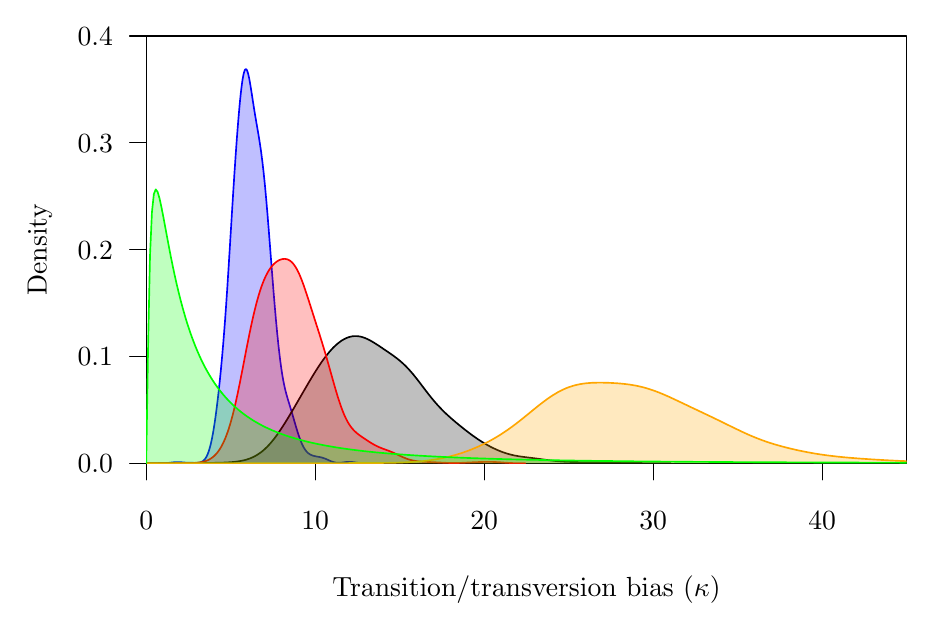
\begin{tikzpicture}[x=1pt,y=1pt]
\definecolor[named]{drawColor}{rgb}{0.00,0.00,0.00}
\definecolor[named]{fillColor}{rgb}{1.00,1.00,1.00}
%\fill[color=fillColor,fill opacity=0.00,] (0,0) rectangle (325.21,216.81);
\begin{scope}
%\path[clip] (  0.00,  0.00) rectangle (325.21,216.81);
\definecolor[named]{drawColor}{rgb}{0.00,0.00,0.00}

\draw[color=drawColor,line cap=round,line join=round,fill opacity=0.00,] ( 49.20, 49.20) -- (293.48, 49.20);

\draw[color=drawColor,line cap=round,line join=round,fill opacity=0.00,] ( 49.20, 49.20) -- ( 49.20, 43.20);

\draw[color=drawColor,line cap=round,line join=round,fill opacity=0.00,] (110.27, 49.20) -- (110.27, 43.20);

\draw[color=drawColor,line cap=round,line join=round,fill opacity=0.00,] (171.34, 49.20) -- (171.34, 43.20);

\draw[color=drawColor,line cap=round,line join=round,fill opacity=0.00,] (232.41, 49.20) -- (232.41, 43.20);

\draw[color=drawColor,line cap=round,line join=round,fill opacity=0.00,] (293.48, 49.20) -- (293.48, 43.20);

\node[color=drawColor,anchor=base,inner sep=0pt, outer sep=0pt, scale=  1.00] at ( 49.20, 25.20) {0};

\node[color=drawColor,anchor=base,inner sep=0pt, outer sep=0pt, scale=  1.00] at (110.27, 25.20) {10};

\node[color=drawColor,anchor=base,inner sep=0pt, outer sep=0pt, scale=  1.00] at (171.34, 25.20) {20};

\node[color=drawColor,anchor=base,inner sep=0pt, outer sep=0pt, scale=  1.00] at (232.41, 25.20) {30};

\node[color=drawColor,anchor=base,inner sep=0pt, outer sep=0pt, scale=  1.00] at (293.48, 25.20) {40};

\draw[color=drawColor,line cap=round,line join=round,fill opacity=0.00,] ( 49.20, 49.20) -- ( 49.20,203.61);

\draw[color=drawColor,line cap=round,line join=round,fill opacity=0.00,] ( 49.20, 49.20) -- ( 43.20, 49.20);

\draw[color=drawColor,line cap=round,line join=round,fill opacity=0.00,] ( 49.20, 87.80) -- ( 43.20, 87.80);

\draw[color=drawColor,line cap=round,line join=round,fill opacity=0.00,] ( 49.20,126.41) -- ( 43.20,126.41);

\draw[color=drawColor,line cap=round,line join=round,fill opacity=0.00,] ( 49.20,165.01) -- ( 43.20,165.01);

\draw[color=drawColor,line cap=round,line join=round,fill opacity=0.00,] ( 49.20,203.61) -- ( 43.20,203.61);

\node[color=drawColor,anchor=base east,inner sep=0pt, outer sep=0pt, scale=  1.00] at ( 37.20, 45.76) {0.0};

\node[color=drawColor,anchor=base east,inner sep=0pt, outer sep=0pt, scale=  1.00] at ( 37.20, 84.36) {0.1};

\node[color=drawColor,anchor=base east,inner sep=0pt, outer sep=0pt, scale=  1.00] at ( 37.20,122.96) {0.2};

\node[color=drawColor,anchor=base east,inner sep=0pt, outer sep=0pt, scale=  1.00] at ( 37.20,161.56) {0.3};

\node[color=drawColor,anchor=base east,inner sep=0pt, outer sep=0pt, scale=  1.00] at ( 37.20,200.17) {0.4};

\draw[color=drawColor,line cap=round,line join=round,fill opacity=0.00,] ( 49.20, 49.20) --
	(324.01, 49.20) --
	(324.01,203.61) --
	( 49.20,203.61) --
	( 49.20, 49.20);
\end{scope}
\begin{scope}
%\path[clip] (  0.00,  0.00) rectangle (325.21,216.81);
\definecolor[named]{drawColor}{rgb}{0.00,0.00,0.00}

\node[color=drawColor,anchor=base,inner sep=0pt, outer sep=0pt, scale=  1.00] at (186.61,  1.20) {Transition/transversion bias ($\kappa$)};

\node[rotate= 90.00,color=drawColor,anchor=base,inner sep=0pt, outer sep=0pt, scale=  1.00] at ( 13.20,126.41) {Density};
\end{scope}
\begin{scope}
\path[clip] ( 49.20, 49.20) rectangle (324.01,203.61);
\definecolor[named]{fillColor}{rgb}{0.00,0.00,1.00}

\draw[fill=fillColor,fill opacity=0.25,draw opacity=0.00,] ( 53.74, 49.20) --
	( 53.88, 49.20) --
	( 54.03, 49.21) --
	( 54.18, 49.21) --
	( 54.32, 49.21) --
	( 54.47, 49.21) --
	( 54.62, 49.21) --
	( 54.76, 49.21) --
	( 54.91, 49.22) --
	( 55.06, 49.22) --
	( 55.20, 49.22) --
	( 55.35, 49.23) --
	( 55.50, 49.23) --
	( 55.65, 49.24) --
	( 55.79, 49.24) --
	( 55.94, 49.25) --
	( 56.09, 49.26) --
	( 56.23, 49.27) --
	( 56.38, 49.28) --
	( 56.53, 49.29) --
	( 56.67, 49.30) --
	( 56.82, 49.31) --
	( 56.97, 49.32) --
	( 57.11, 49.34) --
	( 57.26, 49.35) --
	( 57.41, 49.37) --
	( 57.55, 49.38) --
	( 57.70, 49.40) --
	( 57.85, 49.41) --
	( 58.00, 49.43) --
	( 58.14, 49.45) --
	( 58.29, 49.47) --
	( 58.44, 49.48) --
	( 58.58, 49.50) --
	( 58.73, 49.52) --
	( 58.88, 49.54) --
	( 59.02, 49.55) --
	( 59.17, 49.57) --
	( 59.32, 49.58) --
	( 59.46, 49.59) --
	( 59.61, 49.60) --
	( 59.76, 49.61) --
	( 59.90, 49.62) --
	( 60.05, 49.63) --
	( 60.20, 49.63) --
	( 60.35, 49.63) --
	( 60.49, 49.64) --
	( 60.64, 49.64) --
	( 60.79, 49.63) --
	( 60.93, 49.63) --
	( 61.08, 49.62) --
	( 61.23, 49.62) --
	( 61.37, 49.61) --
	( 61.52, 49.60) --
	( 61.67, 49.59) --
	( 61.81, 49.58) --
	( 61.96, 49.57) --
	( 62.11, 49.56) --
	( 62.25, 49.54) --
	( 62.40, 49.53) --
	( 62.55, 49.52) --
	( 62.69, 49.51) --
	( 62.84, 49.50) --
	( 62.99, 49.48) --
	( 63.14, 49.47) --
	( 63.28, 49.46) --
	( 63.43, 49.46) --
	( 63.58, 49.45) --
	( 63.72, 49.44) --
	( 63.87, 49.43) --
	( 64.02, 49.43) --
	( 64.16, 49.42) --
	( 64.31, 49.41) --
	( 64.46, 49.41) --
	( 64.60, 49.41) --
	( 64.75, 49.40) --
	( 64.90, 49.40) --
	( 65.04, 49.39) --
	( 65.19, 49.39) --
	( 65.34, 49.39) --
	( 65.49, 49.38) --
	( 65.63, 49.38) --
	( 65.78, 49.38) --
	( 65.93, 49.37) --
	( 66.07, 49.37) --
	( 66.22, 49.37) --
	( 66.37, 49.37) --
	( 66.51, 49.36) --
	( 66.66, 49.36) --
	( 66.81, 49.36) --
	( 66.95, 49.36) --
	( 67.10, 49.36) --
	( 67.25, 49.36) --
	( 67.39, 49.36) --
	( 67.54, 49.37) --
	( 67.69, 49.37) --
	( 67.84, 49.38) --
	( 67.98, 49.40) --
	( 68.13, 49.41) --
	( 68.28, 49.44) --
	( 68.42, 49.46) --
	( 68.57, 49.49) --
	( 68.72, 49.53) --
	( 68.86, 49.57) --
	( 69.01, 49.63) --
	( 69.16, 49.69) --
	( 69.30, 49.76) --
	( 69.45, 49.84) --
	( 69.60, 49.93) --
	( 69.74, 50.04) --
	( 69.89, 50.16) --
	( 70.04, 50.29) --
	( 70.19, 50.44) --
	( 70.33, 50.61) --
	( 70.48, 50.80) --
	( 70.63, 51.01) --
	( 70.77, 51.24) --
	( 70.92, 51.49) --
	( 71.07, 51.76) --
	( 71.21, 52.07) --
	( 71.36, 52.41) --
	( 71.51, 52.77) --
	( 71.65, 53.16) --
	( 71.80, 53.58) --
	( 71.95, 54.04) --
	( 72.09, 54.53) --
	( 72.24, 55.05) --
	( 72.39, 55.62) --
	( 72.54, 56.21) --
	( 72.68, 56.85) --
	( 72.83, 57.53) --
	( 72.98, 58.24) --
	( 73.12, 58.99) --
	( 73.27, 59.78) --
	( 73.42, 60.61) --
	( 73.56, 61.48) --
	( 73.71, 62.39) --
	( 73.86, 63.34) --
	( 74.00, 64.32) --
	( 74.15, 65.33) --
	( 74.30, 66.39) --
	( 74.44, 67.48) --
	( 74.59, 68.61) --
	( 74.74, 69.77) --
	( 74.88, 70.96) --
	( 75.03, 72.19) --
	( 75.18, 73.45) --
	( 75.33, 74.75) --
	( 75.47, 76.08) --
	( 75.62, 77.44) --
	( 75.77, 78.84) --
	( 75.91, 80.27) --
	( 76.06, 81.75) --
	( 76.21, 83.26) --
	( 76.35, 84.80) --
	( 76.50, 86.39) --
	( 76.65, 88.02) --
	( 76.79, 89.70) --
	( 76.94, 91.42) --
	( 77.09, 93.19) --
	( 77.23, 95.01) --
	( 77.38, 96.87) --
	( 77.53, 98.78) --
	( 77.68,100.75) --
	( 77.82,102.77) --
	( 77.97,104.83) --
	( 78.12,106.93) --
	( 78.26,109.08) --
	( 78.41,111.28) --
	( 78.56,113.52) --
	( 78.70,115.80) --
	( 78.85,118.10) --
	( 79.00,120.43) --
	( 79.14,122.79) --
	( 79.29,125.17) --
	( 79.44,127.57) --
	( 79.58,129.97) --
	( 79.73,132.38) --
	( 79.88,134.79) --
	( 80.03,137.20) --
	( 80.17,139.59) --
	( 80.32,141.98) --
	( 80.47,144.34) --
	( 80.61,146.68) --
	( 80.76,149.00) --
	( 80.91,151.29) --
	( 81.05,153.54) --
	( 81.20,155.76) --
	( 81.35,157.94) --
	( 81.49,160.09) --
	( 81.64,162.19) --
	( 81.79,164.24) --
	( 81.93,166.25) --
	( 82.08,168.21) --
	( 82.23,170.12) --
	( 82.38,171.97) --
	( 82.52,173.76) --
	( 82.67,175.49) --
	( 82.82,177.16) --
	( 82.96,178.76) --
	( 83.11,180.30) --
	( 83.26,181.74) --
	( 83.40,183.10) --
	( 83.55,184.38) --
	( 83.70,185.58) --
	( 83.84,186.68) --
	( 83.99,187.68) --
	( 84.14,188.56) --
	( 84.28,189.33) --
	( 84.43,190.00) --
	( 84.58,190.56) --
	( 84.72,191.01) --
	( 84.87,191.33) --
	( 85.02,191.53) --
	( 85.17,191.61) --
	( 85.31,191.59) --
	( 85.46,191.46) --
	( 85.61,191.23) --
	( 85.75,190.87) --
	( 85.90,190.43) --
	( 86.05,189.90) --
	( 86.19,189.29) --
	( 86.34,188.62) --
	( 86.49,187.87) --
	( 86.63,187.06) --
	( 86.78,186.21) --
	( 86.93,185.33) --
	( 87.07,184.42) --
	( 87.22,183.48) --
	( 87.37,182.53) --
	( 87.52,181.57) --
	( 87.66,180.62) --
	( 87.81,179.67) --
	( 87.96,178.72) --
	( 88.10,177.79) --
	( 88.25,176.87) --
	( 88.40,175.96) --
	( 88.54,175.07) --
	( 88.69,174.19) --
	( 88.84,173.33) --
	( 88.98,172.47) --
	( 89.13,171.62) --
	( 89.28,170.77) --
	( 89.42,169.92) --
	( 89.57,169.07) --
	( 89.72,168.21) --
	( 89.87,167.33) --
	( 90.01,166.43) --
	( 90.16,165.51) --
	( 90.31,164.56) --
	( 90.45,163.58) --
	( 90.60,162.57) --
	( 90.75,161.51) --
	( 90.89,160.41) --
	( 91.04,159.27) --
	( 91.19,158.09) --
	( 91.33,156.85) --
	( 91.48,155.56) --
	( 91.63,154.22) --
	( 91.77,152.84) --
	( 91.92,151.40) --
	( 92.07,149.92) --
	( 92.22,148.38) --
	( 92.36,146.79) --
	( 92.51,145.16) --
	( 92.66,143.49) --
	( 92.80,141.79) --
	( 92.95,140.04) --
	( 93.10,138.25) --
	( 93.24,136.44) --
	( 93.39,134.60) --
	( 93.54,132.74) --
	( 93.68,130.87) --
	( 93.83,128.97) --
	( 93.98,127.07) --
	( 94.12,125.16) --
	( 94.27,123.25) --
	( 94.42,121.35) --
	( 94.56,119.45) --
	( 94.71,117.56) --
	( 94.86,115.69) --
	( 95.01,113.83) --
	( 95.15,111.99) --
	( 95.30,110.18) --
	( 95.45,108.39) --
	( 95.59,106.64) --
	( 95.74,104.91) --
	( 95.89,103.22) --
	( 96.03,101.56) --
	( 96.18, 99.95) --
	( 96.33, 98.37) --
	( 96.47, 96.84) --
	( 96.62, 95.34) --
	( 96.77, 93.89) --
	( 96.91, 92.48) --
	( 97.06, 91.13) --
	( 97.21, 89.82) --
	( 97.36, 88.56) --
	( 97.50, 87.35) --
	( 97.65, 86.18) --
	( 97.80, 85.07) --
	( 97.94, 84.01) --
	( 98.09, 83.00) --
	( 98.24, 82.03) --
	( 98.38, 81.11) --
	( 98.53, 80.24) --
	( 98.68, 79.42) --
	( 98.82, 78.64) --
	( 98.97, 77.90) --
	( 99.12, 77.20) --
	( 99.26, 76.54) --
	( 99.41, 75.90) --
	( 99.56, 75.31) --
	( 99.71, 74.73) --
	( 99.85, 74.18) --
	(100.00, 73.65) --
	(100.15, 73.13) --
	(100.29, 72.63) --
	(100.44, 72.14) --
	(100.59, 71.65) --
	(100.73, 71.17) --
	(100.88, 70.70) --
	(101.03, 70.22) --
	(101.17, 69.74) --
	(101.32, 69.26) --
	(101.47, 68.77) --
	(101.61, 68.28) --
	(101.76, 67.79) --
	(101.91, 67.29) --
	(102.06, 66.79) --
	(102.20, 66.28) --
	(102.35, 65.77) --
	(102.50, 65.26) --
	(102.64, 64.75) --
	(102.79, 64.24) --
	(102.94, 63.73) --
	(103.08, 63.23) --
	(103.23, 62.72) --
	(103.38, 62.23) --
	(103.52, 61.74) --
	(103.67, 61.25) --
	(103.82, 60.78) --
	(103.96, 60.32) --
	(104.11, 59.86) --
	(104.26, 59.42) --
	(104.41, 58.99) --
	(104.55, 58.57) --
	(104.70, 58.16) --
	(104.85, 57.77) --
	(104.99, 57.38) --
	(105.14, 57.02) --
	(105.29, 56.67) --
	(105.43, 56.33) --
	(105.58, 56.01) --
	(105.73, 55.70) --
	(105.87, 55.40) --
	(106.02, 55.12) --
	(106.17, 54.86) --
	(106.31, 54.61) --
	(106.46, 54.37) --
	(106.61, 54.15) --
	(106.75, 53.94) --
	(106.90, 53.75) --
	(107.05, 53.56) --
	(107.20, 53.39) --
	(107.34, 53.24) --
	(107.49, 53.09) --
	(107.64, 52.96) --
	(107.78, 52.83) --
	(107.93, 52.72) --
	(108.08, 52.62) --
	(108.22, 52.52) --
	(108.37, 52.43) --
	(108.52, 52.35) --
	(108.66, 52.28) --
	(108.81, 52.21) --
	(108.96, 52.15) --
	(109.10, 52.09) --
	(109.25, 52.04) --
	(109.40, 51.99) --
	(109.55, 51.94) --
	(109.69, 51.90) --
	(109.84, 51.86) --
	(109.99, 51.82) --
	(110.13, 51.79) --
	(110.28, 51.76) --
	(110.43, 51.73) --
	(110.57, 51.70) --
	(110.72, 51.67) --
	(110.87, 51.64) --
	(111.01, 51.61) --
	(111.16, 51.59) --
	(111.31, 51.56) --
	(111.45, 51.53) --
	(111.60, 51.51) --
	(111.75, 51.48) --
	(111.90, 51.45) --
	(112.04, 51.42) --
	(112.19, 51.39) --
	(112.34, 51.36) --
	(112.48, 51.32) --
	(112.63, 51.29) --
	(112.78, 51.25) --
	(112.92, 51.20) --
	(113.07, 51.16) --
	(113.22, 51.11) --
	(113.36, 51.06) --
	(113.51, 51.01) --
	(113.66, 50.96) --
	(113.80, 50.90) --
	(113.95, 50.84) --
	(114.10, 50.78) --
	(114.25, 50.72) --
	(114.39, 50.65) --
	(114.54, 50.59) --
	(114.69, 50.52) --
	(114.83, 50.45) --
	(114.98, 50.38) --
	(115.13, 50.32) --
	(115.27, 50.25) --
	(115.42, 50.18) --
	(115.57, 50.12) --
	(115.71, 50.05) --
	(115.86, 49.99) --
	(116.01, 49.93) --
	(116.15, 49.88) --
	(116.30, 49.82) --
	(116.45, 49.77) --
	(116.59, 49.72) --
	(116.74, 49.68) --
	(116.89, 49.63) --
	(117.04, 49.60) --
	(117.18, 49.56) --
	(117.33, 49.53) --
	(117.48, 49.50) --
	(117.62, 49.47) --
	(117.77, 49.45) --
	(117.92, 49.43) --
	(118.06, 49.42) --
	(118.21, 49.40) --
	(118.36, 49.40) --
	(118.50, 49.39) --
	(118.65, 49.39) --
	(118.80, 49.38) --
	(118.94, 49.39) --
	(119.09, 49.39) --
	(119.24, 49.40) --
	(119.39, 49.41) --
	(119.53, 49.42) --
	(119.68, 49.43) --
	(119.83, 49.45) --
	(119.97, 49.47) --
	(120.12, 49.48) --
	(120.27, 49.50) --
	(120.41, 49.52) --
	(120.56, 49.54) --
	(120.71, 49.56) --
	(120.85, 49.58) --
	(121.00, 49.60) --
	(121.15, 49.62) --
	(121.29, 49.64) --
	(121.44, 49.66) --
	(121.59, 49.68) --
	(121.74, 49.69) --
	(121.88, 49.70) --
	(122.03, 49.71) --
	(122.18, 49.72) --
	(122.32, 49.72) --
	(122.47, 49.73) --
	(122.62, 49.73) --
	(122.76, 49.73) --
	(122.91, 49.72) --
	(123.06, 49.71) --
	(123.20, 49.70) --
	(123.35, 49.69) --
	(123.50, 49.68) --
	(123.64, 49.66) --
	(123.79, 49.64) --
	(123.94, 49.62) --
	(124.09, 49.60) --
	(124.23, 49.58) --
	(124.38, 49.56) --
	(124.53, 49.54) --
	(124.67, 49.51) --
	(124.82, 49.49) --
	(124.97, 49.47) --
	(125.11, 49.45) --
	(125.26, 49.43) --
	(125.41, 49.41) --
	(125.55, 49.39) --
	(125.70, 49.37) --
	(125.85, 49.35) --
	(125.99, 49.33) --
	(126.14, 49.32) --
	(126.29, 49.31) --
	(126.44, 49.29) --
	(126.58, 49.28) --
	(126.73, 49.27) --
	(126.88, 49.26) --
	(127.02, 49.25) --
	(127.17, 49.25) --
	(127.32, 49.24) --
	(127.46, 49.23) --
	(127.61, 49.23) --
	(127.76, 49.22) --
	(127.90, 49.22) --
	(128.05, 49.22) --
	(128.20, 49.21) --
	(128.34, 49.21) --
	(128.49, 49.21) --
	(128.64, 49.21) --
	(128.78, 49.21) --
	cycle;
\definecolor[named]{drawColor}{rgb}{0.00,0.00,1.00}

\draw[color=drawColor,line width= 0.6pt,line cap=round,line join=round,fill opacity=0.00,] ( 53.74, 49.20) --
	( 53.88, 49.20) --
	( 54.03, 49.21) --
	( 54.18, 49.21) --
	( 54.32, 49.21) --
	( 54.47, 49.21) --
	( 54.62, 49.21) --
	( 54.76, 49.21) --
	( 54.91, 49.22) --
	( 55.06, 49.22) --
	( 55.20, 49.22) --
	( 55.35, 49.23) --
	( 55.50, 49.23) --
	( 55.65, 49.24) --
	( 55.79, 49.24) --
	( 55.94, 49.25) --
	( 56.09, 49.26) --
	( 56.23, 49.27) --
	( 56.38, 49.28) --
	( 56.53, 49.29) --
	( 56.67, 49.30) --
	( 56.82, 49.31) --
	( 56.97, 49.32) --
	( 57.11, 49.34) --
	( 57.26, 49.35) --
	( 57.41, 49.37) --
	( 57.55, 49.38) --
	( 57.70, 49.40) --
	( 57.85, 49.41) --
	( 58.00, 49.43) --
	( 58.14, 49.45) --
	( 58.29, 49.47) --
	( 58.44, 49.48) --
	( 58.58, 49.50) --
	( 58.73, 49.52) --
	( 58.88, 49.54) --
	( 59.02, 49.55) --
	( 59.17, 49.57) --
	( 59.32, 49.58) --
	( 59.46, 49.59) --
	( 59.61, 49.60) --
	( 59.76, 49.61) --
	( 59.90, 49.62) --
	( 60.05, 49.63) --
	( 60.20, 49.63) --
	( 60.35, 49.63) --
	( 60.49, 49.64) --
	( 60.64, 49.64) --
	( 60.79, 49.63) --
	( 60.93, 49.63) --
	( 61.08, 49.62) --
	( 61.23, 49.62) --
	( 61.37, 49.61) --
	( 61.52, 49.60) --
	( 61.67, 49.59) --
	( 61.81, 49.58) --
	( 61.96, 49.57) --
	( 62.11, 49.56) --
	( 62.25, 49.54) --
	( 62.40, 49.53) --
	( 62.55, 49.52) --
	( 62.69, 49.51) --
	( 62.84, 49.50) --
	( 62.99, 49.48) --
	( 63.14, 49.47) --
	( 63.28, 49.46) --
	( 63.43, 49.46) --
	( 63.58, 49.45) --
	( 63.72, 49.44) --
	( 63.87, 49.43) --
	( 64.02, 49.43) --
	( 64.16, 49.42) --
	( 64.31, 49.41) --
	( 64.46, 49.41) --
	( 64.60, 49.41) --
	( 64.75, 49.40) --
	( 64.90, 49.40) --
	( 65.04, 49.39) --
	( 65.19, 49.39) --
	( 65.34, 49.39) --
	( 65.49, 49.38) --
	( 65.63, 49.38) --
	( 65.78, 49.38) --
	( 65.93, 49.37) --
	( 66.07, 49.37) --
	( 66.22, 49.37) --
	( 66.37, 49.37) --
	( 66.51, 49.36) --
	( 66.66, 49.36) --
	( 66.81, 49.36) --
	( 66.95, 49.36) --
	( 67.10, 49.36) --
	( 67.25, 49.36) --
	( 67.39, 49.36) --
	( 67.54, 49.37) --
	( 67.69, 49.37) --
	( 67.84, 49.38) --
	( 67.98, 49.40) --
	( 68.13, 49.41) --
	( 68.28, 49.44) --
	( 68.42, 49.46) --
	( 68.57, 49.49) --
	( 68.72, 49.53) --
	( 68.86, 49.57) --
	( 69.01, 49.63) --
	( 69.16, 49.69) --
	( 69.30, 49.76) --
	( 69.45, 49.84) --
	( 69.60, 49.93) --
	( 69.74, 50.04) --
	( 69.89, 50.16) --
	( 70.04, 50.29) --
	( 70.19, 50.44) --
	( 70.33, 50.61) --
	( 70.48, 50.80) --
	( 70.63, 51.01) --
	( 70.77, 51.24) --
	( 70.92, 51.49) --
	( 71.07, 51.76) --
	( 71.21, 52.07) --
	( 71.36, 52.41) --
	( 71.51, 52.77) --
	( 71.65, 53.16) --
	( 71.80, 53.58) --
	( 71.95, 54.04) --
	( 72.09, 54.53) --
	( 72.24, 55.05) --
	( 72.39, 55.62) --
	( 72.54, 56.21) --
	( 72.68, 56.85) --
	( 72.83, 57.53) --
	( 72.98, 58.24) --
	( 73.12, 58.99) --
	( 73.27, 59.78) --
	( 73.42, 60.61) --
	( 73.56, 61.48) --
	( 73.71, 62.39) --
	( 73.86, 63.34) --
	( 74.00, 64.32) --
	( 74.15, 65.33) --
	( 74.30, 66.39) --
	( 74.44, 67.48) --
	( 74.59, 68.61) --
	( 74.74, 69.77) --
	( 74.88, 70.96) --
	( 75.03, 72.19) --
	( 75.18, 73.45) --
	( 75.33, 74.75) --
	( 75.47, 76.08) --
	( 75.62, 77.44) --
	( 75.77, 78.84) --
	( 75.91, 80.27) --
	( 76.06, 81.75) --
	( 76.21, 83.26) --
	( 76.35, 84.80) --
	( 76.50, 86.39) --
	( 76.65, 88.02) --
	( 76.79, 89.70) --
	( 76.94, 91.42) --
	( 77.09, 93.19) --
	( 77.23, 95.01) --
	( 77.38, 96.87) --
	( 77.53, 98.78) --
	( 77.68,100.75) --
	( 77.82,102.77) --
	( 77.97,104.83) --
	( 78.12,106.93) --
	( 78.26,109.08) --
	( 78.41,111.28) --
	( 78.56,113.52) --
	( 78.70,115.80) --
	( 78.85,118.10) --
	( 79.00,120.43) --
	( 79.14,122.79) --
	( 79.29,125.17) --
	( 79.44,127.57) --
	( 79.58,129.97) --
	( 79.73,132.38) --
	( 79.88,134.79) --
	( 80.03,137.20) --
	( 80.17,139.59) --
	( 80.32,141.98) --
	( 80.47,144.34) --
	( 80.61,146.68) --
	( 80.76,149.00) --
	( 80.91,151.29) --
	( 81.05,153.54) --
	( 81.20,155.76) --
	( 81.35,157.94) --
	( 81.49,160.09) --
	( 81.64,162.19) --
	( 81.79,164.24) --
	( 81.93,166.25) --
	( 82.08,168.21) --
	( 82.23,170.12) --
	( 82.38,171.97) --
	( 82.52,173.76) --
	( 82.67,175.49) --
	( 82.82,177.16) --
	( 82.96,178.76) --
	( 83.11,180.30) --
	( 83.26,181.74) --
	( 83.40,183.10) --
	( 83.55,184.38) --
	( 83.70,185.58) --
	( 83.84,186.68) --
	( 83.99,187.68) --
	( 84.14,188.56) --
	( 84.28,189.33) --
	( 84.43,190.00) --
	( 84.58,190.56) --
	( 84.72,191.01) --
	( 84.87,191.33) --
	( 85.02,191.53) --
	( 85.17,191.61) --
	( 85.31,191.59) --
	( 85.46,191.46) --
	( 85.61,191.23) --
	( 85.75,190.87) --
	( 85.90,190.43) --
	( 86.05,189.90) --
	( 86.19,189.29) --
	( 86.34,188.62) --
	( 86.49,187.87) --
	( 86.63,187.06) --
	( 86.78,186.21) --
	( 86.93,185.33) --
	( 87.07,184.42) --
	( 87.22,183.48) --
	( 87.37,182.53) --
	( 87.52,181.57) --
	( 87.66,180.62) --
	( 87.81,179.67) --
	( 87.96,178.72) --
	( 88.10,177.79) --
	( 88.25,176.87) --
	( 88.40,175.96) --
	( 88.54,175.07) --
	( 88.69,174.19) --
	( 88.84,173.33) --
	( 88.98,172.47) --
	( 89.13,171.62) --
	( 89.28,170.77) --
	( 89.42,169.92) --
	( 89.57,169.07) --
	( 89.72,168.21) --
	( 89.87,167.33) --
	( 90.01,166.43) --
	( 90.16,165.51) --
	( 90.31,164.56) --
	( 90.45,163.58) --
	( 90.60,162.57) --
	( 90.75,161.51) --
	( 90.89,160.41) --
	( 91.04,159.27) --
	( 91.19,158.09) --
	( 91.33,156.85) --
	( 91.48,155.56) --
	( 91.63,154.22) --
	( 91.77,152.84) --
	( 91.92,151.40) --
	( 92.07,149.92) --
	( 92.22,148.38) --
	( 92.36,146.79) --
	( 92.51,145.16) --
	( 92.66,143.49) --
	( 92.80,141.79) --
	( 92.95,140.04) --
	( 93.10,138.25) --
	( 93.24,136.44) --
	( 93.39,134.60) --
	( 93.54,132.74) --
	( 93.68,130.87) --
	( 93.83,128.97) --
	( 93.98,127.07) --
	( 94.12,125.16) --
	( 94.27,123.25) --
	( 94.42,121.35) --
	( 94.56,119.45) --
	( 94.71,117.56) --
	( 94.86,115.69) --
	( 95.01,113.83) --
	( 95.15,111.99) --
	( 95.30,110.18) --
	( 95.45,108.39) --
	( 95.59,106.64) --
	( 95.74,104.91) --
	( 95.89,103.22) --
	( 96.03,101.56) --
	( 96.18, 99.95) --
	( 96.33, 98.37) --
	( 96.47, 96.84) --
	( 96.62, 95.34) --
	( 96.77, 93.89) --
	( 96.91, 92.48) --
	( 97.06, 91.13) --
	( 97.21, 89.82) --
	( 97.36, 88.56) --
	( 97.50, 87.35) --
	( 97.65, 86.18) --
	( 97.80, 85.07) --
	( 97.94, 84.01) --
	( 98.09, 83.00) --
	( 98.24, 82.03) --
	( 98.38, 81.11) --
	( 98.53, 80.24) --
	( 98.68, 79.42) --
	( 98.82, 78.64) --
	( 98.97, 77.90) --
	( 99.12, 77.20) --
	( 99.26, 76.54) --
	( 99.41, 75.90) --
	( 99.56, 75.31) --
	( 99.71, 74.73) --
	( 99.85, 74.18) --
	(100.00, 73.65) --
	(100.15, 73.13) --
	(100.29, 72.63) --
	(100.44, 72.14) --
	(100.59, 71.65) --
	(100.73, 71.17) --
	(100.88, 70.70) --
	(101.03, 70.22) --
	(101.17, 69.74) --
	(101.32, 69.26) --
	(101.47, 68.77) --
	(101.61, 68.28) --
	(101.76, 67.79) --
	(101.91, 67.29) --
	(102.06, 66.79) --
	(102.20, 66.28) --
	(102.35, 65.77) --
	(102.50, 65.26) --
	(102.64, 64.75) --
	(102.79, 64.24) --
	(102.94, 63.73) --
	(103.08, 63.23) --
	(103.23, 62.72) --
	(103.38, 62.23) --
	(103.52, 61.74) --
	(103.67, 61.25) --
	(103.82, 60.78) --
	(103.96, 60.32) --
	(104.11, 59.86) --
	(104.26, 59.42) --
	(104.41, 58.99) --
	(104.55, 58.57) --
	(104.70, 58.16) --
	(104.85, 57.77) --
	(104.99, 57.38) --
	(105.14, 57.02) --
	(105.29, 56.67) --
	(105.43, 56.33) --
	(105.58, 56.01) --
	(105.73, 55.70) --
	(105.87, 55.40) --
	(106.02, 55.12) --
	(106.17, 54.86) --
	(106.31, 54.61) --
	(106.46, 54.37) --
	(106.61, 54.15) --
	(106.75, 53.94) --
	(106.90, 53.75) --
	(107.05, 53.56) --
	(107.20, 53.39) --
	(107.34, 53.24) --
	(107.49, 53.09) --
	(107.64, 52.96) --
	(107.78, 52.83) --
	(107.93, 52.72) --
	(108.08, 52.62) --
	(108.22, 52.52) --
	(108.37, 52.43) --
	(108.52, 52.35) --
	(108.66, 52.28) --
	(108.81, 52.21) --
	(108.96, 52.15) --
	(109.10, 52.09) --
	(109.25, 52.04) --
	(109.40, 51.99) --
	(109.55, 51.94) --
	(109.69, 51.90) --
	(109.84, 51.86) --
	(109.99, 51.82) --
	(110.13, 51.79) --
	(110.28, 51.76) --
	(110.43, 51.73) --
	(110.57, 51.70) --
	(110.72, 51.67) --
	(110.87, 51.64) --
	(111.01, 51.61) --
	(111.16, 51.59) --
	(111.31, 51.56) --
	(111.45, 51.53) --
	(111.60, 51.51) --
	(111.75, 51.48) --
	(111.90, 51.45) --
	(112.04, 51.42) --
	(112.19, 51.39) --
	(112.34, 51.36) --
	(112.48, 51.32) --
	(112.63, 51.29) --
	(112.78, 51.25) --
	(112.92, 51.20) --
	(113.07, 51.16) --
	(113.22, 51.11) --
	(113.36, 51.06) --
	(113.51, 51.01) --
	(113.66, 50.96) --
	(113.80, 50.90) --
	(113.95, 50.84) --
	(114.10, 50.78) --
	(114.25, 50.72) --
	(114.39, 50.65) --
	(114.54, 50.59) --
	(114.69, 50.52) --
	(114.83, 50.45) --
	(114.98, 50.38) --
	(115.13, 50.32) --
	(115.27, 50.25) --
	(115.42, 50.18) --
	(115.57, 50.12) --
	(115.71, 50.05) --
	(115.86, 49.99) --
	(116.01, 49.93) --
	(116.15, 49.88) --
	(116.30, 49.82) --
	(116.45, 49.77) --
	(116.59, 49.72) --
	(116.74, 49.68) --
	(116.89, 49.63) --
	(117.04, 49.60) --
	(117.18, 49.56) --
	(117.33, 49.53) --
	(117.48, 49.50) --
	(117.62, 49.47) --
	(117.77, 49.45) --
	(117.92, 49.43) --
	(118.06, 49.42) --
	(118.21, 49.40) --
	(118.36, 49.40) --
	(118.50, 49.39) --
	(118.65, 49.39) --
	(118.80, 49.38) --
	(118.94, 49.39) --
	(119.09, 49.39) --
	(119.24, 49.40) --
	(119.39, 49.41) --
	(119.53, 49.42) --
	(119.68, 49.43) --
	(119.83, 49.45) --
	(119.97, 49.47) --
	(120.12, 49.48) --
	(120.27, 49.50) --
	(120.41, 49.52) --
	(120.56, 49.54) --
	(120.71, 49.56) --
	(120.85, 49.58) --
	(121.00, 49.60) --
	(121.15, 49.62) --
	(121.29, 49.64) --
	(121.44, 49.66) --
	(121.59, 49.68) --
	(121.74, 49.69) --
	(121.88, 49.70) --
	(122.03, 49.71) --
	(122.18, 49.72) --
	(122.32, 49.72) --
	(122.47, 49.73) --
	(122.62, 49.73) --
	(122.76, 49.73) --
	(122.91, 49.72) --
	(123.06, 49.71) --
	(123.20, 49.70) --
	(123.35, 49.69) --
	(123.50, 49.68) --
	(123.64, 49.66) --
	(123.79, 49.64) --
	(123.94, 49.62) --
	(124.09, 49.60) --
	(124.23, 49.58) --
	(124.38, 49.56) --
	(124.53, 49.54) --
	(124.67, 49.51) --
	(124.82, 49.49) --
	(124.97, 49.47) --
	(125.11, 49.45) --
	(125.26, 49.43) --
	(125.41, 49.41) --
	(125.55, 49.39) --
	(125.70, 49.37) --
	(125.85, 49.35) --
	(125.99, 49.33) --
	(126.14, 49.32) --
	(126.29, 49.31) --
	(126.44, 49.29) --
	(126.58, 49.28) --
	(126.73, 49.27) --
	(126.88, 49.26) --
	(127.02, 49.25) --
	(127.17, 49.25) --
	(127.32, 49.24) --
	(127.46, 49.23) --
	(127.61, 49.23) --
	(127.76, 49.22) --
	(127.90, 49.22) --
	(128.05, 49.22) --
	(128.20, 49.21) --
	(128.34, 49.21) --
	(128.49, 49.21) --
	(128.64, 49.21) --
	(128.78, 49.21);
\definecolor[named]{fillColor}{rgb}{0.00,0.00,0.00}

\draw[fill=fillColor,fill opacity=0.25,draw opacity=0.00,] ( 42.47, 49.20) --
	( 42.85, 49.20) --
	( 43.23, 49.20) --
	( 43.62, 49.20) --
	( 44.00, 49.20) --
	( 44.39, 49.20) --
	( 44.77, 49.20) --
	( 45.15, 49.20) --
	( 45.54, 49.20) --
	( 45.92, 49.20) --
	( 46.31, 49.20) --
	( 46.69, 49.20) --
	( 47.08, 49.20) --
	( 47.46, 49.20) --
	( 47.84, 49.20) --
	( 48.23, 49.21) --
	( 48.61, 49.21) --
	( 49.00, 49.21) --
	( 49.38, 49.21) --
	( 49.76, 49.21) --
	( 50.15, 49.21) --
	( 50.53, 49.21) --
	( 50.92, 49.21) --
	( 51.30, 49.22) --
	( 51.68, 49.22) --
	( 52.07, 49.22) --
	( 52.45, 49.22) --
	( 52.84, 49.22) --
	( 53.22, 49.23) --
	( 53.61, 49.23) --
	( 53.99, 49.23) --
	( 54.37, 49.24) --
	( 54.76, 49.24) --
	( 55.14, 49.24) --
	( 55.53, 49.25) --
	( 55.91, 49.25) --
	( 56.29, 49.25) --
	( 56.68, 49.26) --
	( 57.06, 49.26) --
	( 57.45, 49.26) --
	( 57.83, 49.27) --
	( 58.22, 49.27) --
	( 58.60, 49.28) --
	( 58.98, 49.28) --
	( 59.37, 49.28) --
	( 59.75, 49.29) --
	( 60.14, 49.29) --
	( 60.52, 49.29) --
	( 60.90, 49.30) --
	( 61.29, 49.30) --
	( 61.67, 49.30) --
	( 62.06, 49.31) --
	( 62.44, 49.31) --
	( 62.82, 49.31) --
	( 63.21, 49.31) --
	( 63.59, 49.31) --
	( 63.98, 49.32) --
	( 64.36, 49.32) --
	( 64.75, 49.32) --
	( 65.13, 49.32) --
	( 65.51, 49.32) --
	( 65.90, 49.32) --
	( 66.28, 49.32) --
	( 66.67, 49.32) --
	( 67.05, 49.32) --
	( 67.43, 49.32) --
	( 67.82, 49.32) --
	( 68.20, 49.32) --
	( 68.59, 49.32) --
	( 68.97, 49.33) --
	( 69.36, 49.33) --
	( 69.74, 49.33) --
	( 70.12, 49.33) --
	( 70.51, 49.33) --
	( 70.89, 49.33) --
	( 71.28, 49.34) --
	( 71.66, 49.34) --
	( 72.04, 49.34) --
	( 72.43, 49.35) --
	( 72.81, 49.35) --
	( 73.20, 49.36) --
	( 73.58, 49.36) --
	( 73.96, 49.37) --
	( 74.35, 49.37) --
	( 74.73, 49.38) --
	( 75.12, 49.39) --
	( 75.50, 49.40) --
	( 75.89, 49.41) --
	( 76.27, 49.42) --
	( 76.65, 49.44) --
	( 77.04, 49.45) --
	( 77.42, 49.47) --
	( 77.81, 49.48) --
	( 78.19, 49.50) --
	( 78.57, 49.52) --
	( 78.96, 49.55) --
	( 79.34, 49.57) --
	( 79.73, 49.60) --
	( 80.11, 49.63) --
	( 80.50, 49.66) --
	( 80.88, 49.70) --
	( 81.26, 49.74) --
	( 81.65, 49.79) --
	( 82.03, 49.84) --
	( 82.42, 49.89) --
	( 82.80, 49.95) --
	( 83.18, 50.02) --
	( 83.57, 50.09) --
	( 83.95, 50.17) --
	( 84.34, 50.25) --
	( 84.72, 50.35) --
	( 85.11, 50.45) --
	( 85.49, 50.56) --
	( 85.87, 50.68) --
	( 86.26, 50.81) --
	( 86.64, 50.95) --
	( 87.03, 51.10) --
	( 87.41, 51.26) --
	( 87.79, 51.44) --
	( 88.18, 51.63) --
	( 88.56, 51.83) --
	( 88.95, 52.05) --
	( 89.33, 52.27) --
	( 89.71, 52.52) --
	( 90.10, 52.78) --
	( 90.48, 53.05) --
	( 90.87, 53.35) --
	( 91.25, 53.65) --
	( 91.64, 53.98) --
	( 92.02, 54.32) --
	( 92.40, 54.68) --
	( 92.79, 55.05) --
	( 93.17, 55.44) --
	( 93.56, 55.85) --
	( 93.94, 56.28) --
	( 94.32, 56.72) --
	( 94.71, 57.18) --
	( 95.09, 57.65) --
	( 95.48, 58.14) --
	( 95.86, 58.64) --
	( 96.25, 59.16) --
	( 96.63, 59.70) --
	( 97.01, 60.24) --
	( 97.40, 60.80) --
	( 97.78, 61.37) --
	( 98.17, 61.95) --
	( 98.55, 62.54) --
	( 98.93, 63.14) --
	( 99.32, 63.75) --
	( 99.70, 64.37) --
	(100.09, 65.00) --
	(100.47, 65.63) --
	(100.85, 66.26) --
	(101.24, 66.90) --
	(101.62, 67.55) --
	(102.01, 68.20) --
	(102.39, 68.86) --
	(102.78, 69.52) --
	(103.16, 70.18) --
	(103.54, 70.84) --
	(103.93, 71.50) --
	(104.31, 72.17) --
	(104.70, 72.83) --
	(105.08, 73.50) --
	(105.46, 74.16) --
	(105.85, 74.82) --
	(106.23, 75.49) --
	(106.62, 76.15) --
	(107.00, 76.81) --
	(107.39, 77.47) --
	(107.77, 78.12) --
	(108.15, 78.77) --
	(108.54, 79.41) --
	(108.92, 80.06) --
	(109.31, 80.69) --
	(109.69, 81.32) --
	(110.07, 81.94) --
	(110.46, 82.56) --
	(110.84, 83.16) --
	(111.23, 83.76) --
	(111.61, 84.34) --
	(111.99, 84.92) --
	(112.38, 85.49) --
	(112.76, 86.04) --
	(113.15, 86.58) --
	(113.53, 87.10) --
	(113.92, 87.62) --
	(114.30, 88.12) --
	(114.68, 88.60) --
	(115.07, 89.07) --
	(115.45, 89.53) --
	(115.84, 89.97) --
	(116.22, 90.39) --
	(116.60, 90.80) --
	(116.99, 91.19) --
	(117.37, 91.56) --
	(117.76, 91.91) --
	(118.14, 92.25) --
	(118.53, 92.57) --
	(118.91, 92.87) --
	(119.29, 93.16) --
	(119.68, 93.43) --
	(120.06, 93.68) --
	(120.45, 93.90) --
	(120.83, 94.11) --
	(121.21, 94.31) --
	(121.60, 94.48) --
	(121.98, 94.64) --
	(122.37, 94.77) --
	(122.75, 94.88) --
	(123.13, 94.98) --
	(123.52, 95.06) --
	(123.90, 95.12) --
	(124.29, 95.15) --
	(124.67, 95.17) --
	(125.06, 95.17) --
	(125.44, 95.15) --
	(125.82, 95.11) --
	(126.21, 95.06) --
	(126.59, 94.98) --
	(126.98, 94.89) --
	(127.36, 94.78) --
	(127.74, 94.66) --
	(128.13, 94.52) --
	(128.51, 94.36) --
	(128.90, 94.20) --
	(129.28, 94.02) --
	(129.67, 93.83) --
	(130.05, 93.62) --
	(130.43, 93.41) --
	(130.82, 93.19) --
	(131.20, 92.97) --
	(131.59, 92.73) --
	(131.97, 92.49) --
	(132.35, 92.24) --
	(132.74, 92.00) --
	(133.12, 91.75) --
	(133.51, 91.49) --
	(133.89, 91.23) --
	(134.28, 90.98) --
	(134.66, 90.72) --
	(135.04, 90.46) --
	(135.43, 90.20) --
	(135.81, 89.94) --
	(136.20, 89.68) --
	(136.58, 89.42) --
	(136.96, 89.15) --
	(137.35, 88.89) --
	(137.73, 88.62) --
	(138.12, 88.35) --
	(138.50, 88.08) --
	(138.88, 87.80) --
	(139.27, 87.51) --
	(139.65, 87.22) --
	(140.04, 86.92) --
	(140.42, 86.61) --
	(140.81, 86.30) --
	(141.19, 85.97) --
	(141.57, 85.63) --
	(141.96, 85.29) --
	(142.34, 84.93) --
	(142.73, 84.56) --
	(143.11, 84.18) --
	(143.49, 83.78) --
	(143.88, 83.38) --
	(144.26, 82.96) --
	(144.65, 82.53) --
	(145.03, 82.09) --
	(145.42, 81.64) --
	(145.80, 81.18) --
	(146.18, 80.71) --
	(146.57, 80.23) --
	(146.95, 79.74) --
	(147.34, 79.25) --
	(147.72, 78.75) --
	(148.10, 78.25) --
	(148.49, 77.74) --
	(148.87, 77.24) --
	(149.26, 76.73) --
	(149.64, 76.22) --
	(150.02, 75.72) --
	(150.41, 75.22) --
	(150.79, 74.72) --
	(151.18, 74.22) --
	(151.56, 73.73) --
	(151.95, 73.25) --
	(152.33, 72.78) --
	(152.71, 72.31) --
	(153.10, 71.85) --
	(153.48, 71.40) --
	(153.87, 70.95) --
	(154.25, 70.52) --
	(154.63, 70.09) --
	(155.02, 69.68) --
	(155.40, 69.27) --
	(155.79, 68.87) --
	(156.17, 68.47) --
	(156.56, 68.09) --
	(156.94, 67.71) --
	(157.32, 67.34) --
	(157.71, 66.98) --
	(158.09, 66.63) --
	(158.48, 66.27) --
	(158.86, 65.93) --
	(159.24, 65.59) --
	(159.63, 65.25) --
	(160.01, 64.92) --
	(160.40, 64.59) --
	(160.78, 64.27) --
	(161.16, 63.94) --
	(161.55, 63.62) --
	(161.93, 63.31) --
	(162.32, 62.99) --
	(162.70, 62.68) --
	(163.09, 62.37) --
	(163.47, 62.06) --
	(163.85, 61.75) --
	(164.24, 61.45) --
	(164.62, 61.15) --
	(165.01, 60.85) --
	(165.39, 60.55) --
	(165.77, 60.26) --
	(166.16, 59.97) --
	(166.54, 59.68) --
	(166.93, 59.40) --
	(167.31, 59.12) --
	(167.70, 58.85) --
	(168.08, 58.58) --
	(168.46, 58.31) --
	(168.85, 58.05) --
	(169.23, 57.79) --
	(169.62, 57.54) --
	(170.00, 57.29) --
	(170.38, 57.04) --
	(170.77, 56.81) --
	(171.15, 56.57) --
	(171.54, 56.34) --
	(171.92, 56.12) --
	(172.30, 55.90) --
	(172.69, 55.69) --
	(173.07, 55.48) --
	(173.46, 55.27) --
	(173.84, 55.07) --
	(174.23, 54.88) --
	(174.61, 54.69) --
	(174.99, 54.51) --
	(175.38, 54.33) --
	(175.76, 54.15) --
	(176.15, 53.98) --
	(176.53, 53.82) --
	(176.91, 53.66) --
	(177.30, 53.51) --
	(177.68, 53.36) --
	(178.07, 53.22) --
	(178.45, 53.08) --
	(178.84, 52.95) --
	(179.22, 52.83) --
	(179.60, 52.71) --
	(179.99, 52.59) --
	(180.37, 52.49) --
	(180.76, 52.39) --
	(181.14, 52.29) --
	(181.52, 52.20) --
	(181.91, 52.11) --
	(182.29, 52.03) --
	(182.68, 51.96) --
	(183.06, 51.89) --
	(183.45, 51.82) --
	(183.83, 51.75) --
	(184.21, 51.69) --
	(184.60, 51.64) --
	(184.98, 51.58) --
	(185.37, 51.53) --
	(185.75, 51.48) --
	(186.13, 51.43) --
	(186.52, 51.38) --
	(186.90, 51.33) --
	(187.29, 51.29) --
	(187.67, 51.24) --
	(188.05, 51.19) --
	(188.44, 51.15) --
	(188.82, 51.10) --
	(189.21, 51.05) --
	(189.59, 51.00) --
	(189.98, 50.95) --
	(190.36, 50.90) --
	(190.74, 50.85) --
	(191.13, 50.80) --
	(191.51, 50.75) --
	(191.90, 50.69) --
	(192.28, 50.64) --
	(192.66, 50.59) --
	(193.05, 50.54) --
	(193.43, 50.48) --
	(193.82, 50.43) --
	(194.20, 50.38) --
	(194.59, 50.33) --
	(194.97, 50.28) --
	(195.35, 50.23) --
	(195.74, 50.19) --
	(196.12, 50.14) --
	(196.51, 50.10) --
	(196.89, 50.06) --
	(197.27, 50.02) --
	(197.66, 49.98) --
	(198.04, 49.95) --
	(198.43, 49.91) --
	(198.81, 49.88) --
	(199.19, 49.86) --
	(199.58, 49.83) --
	(199.96, 49.80) --
	(200.35, 49.78) --
	(200.73, 49.76) --
	(201.12, 49.74) --
	(201.50, 49.73) --
	(201.88, 49.71) --
	(202.27, 49.70) --
	(202.65, 49.69) --
	(203.04, 49.68) --
	(203.42, 49.67) --
	(203.80, 49.66) --
	(204.19, 49.66) --
	(204.57, 49.65) --
	(204.96, 49.65) --
	(205.34, 49.64) --
	(205.73, 49.64) --
	(206.11, 49.64) --
	(206.49, 49.64) --
	(206.88, 49.64) --
	(207.26, 49.63) --
	(207.65, 49.63) --
	(208.03, 49.63) --
	(208.41, 49.63) --
	(208.80, 49.63) --
	(209.18, 49.63) --
	(209.57, 49.63) --
	(209.95, 49.63) --
	(210.33, 49.63) --
	(210.72, 49.63) --
	(211.10, 49.63) --
	(211.49, 49.63) --
	(211.87, 49.63) --
	(212.26, 49.63) --
	(212.64, 49.63) --
	(213.02, 49.62) --
	(213.41, 49.62) --
	(213.79, 49.62) --
	(214.18, 49.62) --
	(214.56, 49.61) --
	(214.94, 49.61) --
	(215.33, 49.60) --
	(215.71, 49.60) --
	(216.10, 49.59) --
	(216.48, 49.59) --
	(216.87, 49.58) --
	(217.25, 49.57) --
	(217.63, 49.57) --
	(218.02, 49.56) --
	(218.40, 49.55) --
	(218.79, 49.54) --
	(219.17, 49.53) --
	(219.55, 49.52) --
	(219.94, 49.51) --
	(220.32, 49.50) --
	(220.71, 49.49) --
	(221.09, 49.48) --
	(221.47, 49.47) --
	(221.86, 49.46) --
	(222.24, 49.44) --
	(222.63, 49.43) --
	(223.01, 49.42) --
	(223.40, 49.41) --
	(223.78, 49.40) --
	(224.16, 49.39) --
	(224.55, 49.38) --
	(224.93, 49.36) --
	(225.32, 49.35) --
	(225.70, 49.34) --
	(226.08, 49.33) --
	(226.47, 49.32) --
	(226.85, 49.31) --
	(227.24, 49.30) --
	(227.62, 49.30) --
	(228.01, 49.29) --
	(228.39, 49.28) --
	(228.77, 49.27) --
	(229.16, 49.27) --
	(229.54, 49.26) --
	(229.93, 49.25) --
	(230.31, 49.25) --
	(230.69, 49.24) --
	(231.08, 49.24) --
	(231.46, 49.23) --
	(231.85, 49.23) --
	(232.23, 49.23) --
	(232.62, 49.22) --
	(233.00, 49.22) --
	(233.38, 49.22) --
	(233.77, 49.22) --
	(234.15, 49.21) --
	(234.54, 49.21) --
	(234.92, 49.21) --
	(235.30, 49.21) --
	(235.69, 49.21) --
	(236.07, 49.21) --
	(236.46, 49.21) --
	(236.84, 49.20) --
	(237.22, 49.20) --
	(237.61, 49.20) --
	(237.99, 49.20) --
	(238.38, 49.20) --
	(238.76, 49.20) --
	cycle;
\definecolor[named]{drawColor}{rgb}{0.00,0.00,0.00}

\draw[color=drawColor,line width= 0.6pt,line cap=round,line join=round,fill opacity=0.00,] ( 42.47, 49.20) --
	( 42.85, 49.20) --
	( 43.23, 49.20) --
	( 43.62, 49.20) --
	( 44.00, 49.20) --
	( 44.39, 49.20) --
	( 44.77, 49.20) --
	( 45.15, 49.20) --
	( 45.54, 49.20) --
	( 45.92, 49.20) --
	( 46.31, 49.20) --
	( 46.69, 49.20) --
	( 47.08, 49.20) --
	( 47.46, 49.20) --
	( 47.84, 49.20) --
	( 48.23, 49.21) --
	( 48.61, 49.21) --
	( 49.00, 49.21) --
	( 49.38, 49.21) --
	( 49.76, 49.21) --
	( 50.15, 49.21) --
	( 50.53, 49.21) --
	( 50.92, 49.21) --
	( 51.30, 49.22) --
	( 51.68, 49.22) --
	( 52.07, 49.22) --
	( 52.45, 49.22) --
	( 52.84, 49.22) --
	( 53.22, 49.23) --
	( 53.61, 49.23) --
	( 53.99, 49.23) --
	( 54.37, 49.24) --
	( 54.76, 49.24) --
	( 55.14, 49.24) --
	( 55.53, 49.25) --
	( 55.91, 49.25) --
	( 56.29, 49.25) --
	( 56.68, 49.26) --
	( 57.06, 49.26) --
	( 57.45, 49.26) --
	( 57.83, 49.27) --
	( 58.22, 49.27) --
	( 58.60, 49.28) --
	( 58.98, 49.28) --
	( 59.37, 49.28) --
	( 59.75, 49.29) --
	( 60.14, 49.29) --
	( 60.52, 49.29) --
	( 60.90, 49.30) --
	( 61.29, 49.30) --
	( 61.67, 49.30) --
	( 62.06, 49.31) --
	( 62.44, 49.31) --
	( 62.82, 49.31) --
	( 63.21, 49.31) --
	( 63.59, 49.31) --
	( 63.98, 49.32) --
	( 64.36, 49.32) --
	( 64.75, 49.32) --
	( 65.13, 49.32) --
	( 65.51, 49.32) --
	( 65.90, 49.32) --
	( 66.28, 49.32) --
	( 66.67, 49.32) --
	( 67.05, 49.32) --
	( 67.43, 49.32) --
	( 67.82, 49.32) --
	( 68.20, 49.32) --
	( 68.59, 49.32) --
	( 68.97, 49.33) --
	( 69.36, 49.33) --
	( 69.74, 49.33) --
	( 70.12, 49.33) --
	( 70.51, 49.33) --
	( 70.89, 49.33) --
	( 71.28, 49.34) --
	( 71.66, 49.34) --
	( 72.04, 49.34) --
	( 72.43, 49.35) --
	( 72.81, 49.35) --
	( 73.20, 49.36) --
	( 73.58, 49.36) --
	( 73.96, 49.37) --
	( 74.35, 49.37) --
	( 74.73, 49.38) --
	( 75.12, 49.39) --
	( 75.50, 49.40) --
	( 75.89, 49.41) --
	( 76.27, 49.42) --
	( 76.65, 49.44) --
	( 77.04, 49.45) --
	( 77.42, 49.47) --
	( 77.81, 49.48) --
	( 78.19, 49.50) --
	( 78.57, 49.52) --
	( 78.96, 49.55) --
	( 79.34, 49.57) --
	( 79.73, 49.60) --
	( 80.11, 49.63) --
	( 80.50, 49.66) --
	( 80.88, 49.70) --
	( 81.26, 49.74) --
	( 81.65, 49.79) --
	( 82.03, 49.84) --
	( 82.42, 49.89) --
	( 82.80, 49.95) --
	( 83.18, 50.02) --
	( 83.57, 50.09) --
	( 83.95, 50.17) --
	( 84.34, 50.25) --
	( 84.72, 50.35) --
	( 85.11, 50.45) --
	( 85.49, 50.56) --
	( 85.87, 50.68) --
	( 86.26, 50.81) --
	( 86.64, 50.95) --
	( 87.03, 51.10) --
	( 87.41, 51.26) --
	( 87.79, 51.44) --
	( 88.18, 51.63) --
	( 88.56, 51.83) --
	( 88.95, 52.05) --
	( 89.33, 52.27) --
	( 89.71, 52.52) --
	( 90.10, 52.78) --
	( 90.48, 53.05) --
	( 90.87, 53.35) --
	( 91.25, 53.65) --
	( 91.64, 53.98) --
	( 92.02, 54.32) --
	( 92.40, 54.68) --
	( 92.79, 55.05) --
	( 93.17, 55.44) --
	( 93.56, 55.85) --
	( 93.94, 56.28) --
	( 94.32, 56.72) --
	( 94.71, 57.18) --
	( 95.09, 57.65) --
	( 95.48, 58.14) --
	( 95.86, 58.64) --
	( 96.25, 59.16) --
	( 96.63, 59.70) --
	( 97.01, 60.24) --
	( 97.40, 60.80) --
	( 97.78, 61.37) --
	( 98.17, 61.95) --
	( 98.55, 62.54) --
	( 98.93, 63.14) --
	( 99.32, 63.75) --
	( 99.70, 64.37) --
	(100.09, 65.00) --
	(100.47, 65.63) --
	(100.85, 66.26) --
	(101.24, 66.90) --
	(101.62, 67.55) --
	(102.01, 68.20) --
	(102.39, 68.86) --
	(102.78, 69.52) --
	(103.16, 70.18) --
	(103.54, 70.84) --
	(103.93, 71.50) --
	(104.31, 72.17) --
	(104.70, 72.83) --
	(105.08, 73.50) --
	(105.46, 74.16) --
	(105.85, 74.82) --
	(106.23, 75.49) --
	(106.62, 76.15) --
	(107.00, 76.81) --
	(107.39, 77.47) --
	(107.77, 78.12) --
	(108.15, 78.77) --
	(108.54, 79.41) --
	(108.92, 80.06) --
	(109.31, 80.69) --
	(109.69, 81.32) --
	(110.07, 81.94) --
	(110.46, 82.56) --
	(110.84, 83.16) --
	(111.23, 83.76) --
	(111.61, 84.34) --
	(111.99, 84.92) --
	(112.38, 85.49) --
	(112.76, 86.04) --
	(113.15, 86.58) --
	(113.53, 87.10) --
	(113.92, 87.62) --
	(114.30, 88.12) --
	(114.68, 88.60) --
	(115.07, 89.07) --
	(115.45, 89.53) --
	(115.84, 89.97) --
	(116.22, 90.39) --
	(116.60, 90.80) --
	(116.99, 91.19) --
	(117.37, 91.56) --
	(117.76, 91.91) --
	(118.14, 92.25) --
	(118.53, 92.57) --
	(118.91, 92.87) --
	(119.29, 93.16) --
	(119.68, 93.43) --
	(120.06, 93.68) --
	(120.45, 93.90) --
	(120.83, 94.11) --
	(121.21, 94.31) --
	(121.60, 94.48) --
	(121.98, 94.64) --
	(122.37, 94.77) --
	(122.75, 94.88) --
	(123.13, 94.98) --
	(123.52, 95.06) --
	(123.90, 95.12) --
	(124.29, 95.15) --
	(124.67, 95.17) --
	(125.06, 95.17) --
	(125.44, 95.15) --
	(125.82, 95.11) --
	(126.21, 95.06) --
	(126.59, 94.98) --
	(126.98, 94.89) --
	(127.36, 94.78) --
	(127.74, 94.66) --
	(128.13, 94.52) --
	(128.51, 94.36) --
	(128.90, 94.20) --
	(129.28, 94.02) --
	(129.67, 93.83) --
	(130.05, 93.62) --
	(130.43, 93.41) --
	(130.82, 93.19) --
	(131.20, 92.97) --
	(131.59, 92.73) --
	(131.97, 92.49) --
	(132.35, 92.24) --
	(132.74, 92.00) --
	(133.12, 91.75) --
	(133.51, 91.49) --
	(133.89, 91.23) --
	(134.28, 90.98) --
	(134.66, 90.72) --
	(135.04, 90.46) --
	(135.43, 90.20) --
	(135.81, 89.94) --
	(136.20, 89.68) --
	(136.58, 89.42) --
	(136.96, 89.15) --
	(137.35, 88.89) --
	(137.73, 88.62) --
	(138.12, 88.35) --
	(138.50, 88.08) --
	(138.88, 87.80) --
	(139.27, 87.51) --
	(139.65, 87.22) --
	(140.04, 86.92) --
	(140.42, 86.61) --
	(140.81, 86.30) --
	(141.19, 85.97) --
	(141.57, 85.63) --
	(141.96, 85.29) --
	(142.34, 84.93) --
	(142.73, 84.56) --
	(143.11, 84.18) --
	(143.49, 83.78) --
	(143.88, 83.38) --
	(144.26, 82.96) --
	(144.65, 82.53) --
	(145.03, 82.09) --
	(145.42, 81.64) --
	(145.80, 81.18) --
	(146.18, 80.71) --
	(146.57, 80.23) --
	(146.95, 79.74) --
	(147.34, 79.25) --
	(147.72, 78.75) --
	(148.10, 78.25) --
	(148.49, 77.74) --
	(148.87, 77.24) --
	(149.26, 76.73) --
	(149.64, 76.22) --
	(150.02, 75.72) --
	(150.41, 75.22) --
	(150.79, 74.72) --
	(151.18, 74.22) --
	(151.56, 73.73) --
	(151.95, 73.25) --
	(152.33, 72.78) --
	(152.71, 72.31) --
	(153.10, 71.85) --
	(153.48, 71.40) --
	(153.87, 70.95) --
	(154.25, 70.52) --
	(154.63, 70.09) --
	(155.02, 69.68) --
	(155.40, 69.27) --
	(155.79, 68.87) --
	(156.17, 68.47) --
	(156.56, 68.09) --
	(156.94, 67.71) --
	(157.32, 67.34) --
	(157.71, 66.98) --
	(158.09, 66.63) --
	(158.48, 66.27) --
	(158.86, 65.93) --
	(159.24, 65.59) --
	(159.63, 65.25) --
	(160.01, 64.92) --
	(160.40, 64.59) --
	(160.78, 64.27) --
	(161.16, 63.94) --
	(161.55, 63.62) --
	(161.93, 63.31) --
	(162.32, 62.99) --
	(162.70, 62.68) --
	(163.09, 62.37) --
	(163.47, 62.06) --
	(163.85, 61.75) --
	(164.24, 61.45) --
	(164.62, 61.15) --
	(165.01, 60.85) --
	(165.39, 60.55) --
	(165.77, 60.26) --
	(166.16, 59.97) --
	(166.54, 59.68) --
	(166.93, 59.40) --
	(167.31, 59.12) --
	(167.70, 58.85) --
	(168.08, 58.58) --
	(168.46, 58.31) --
	(168.85, 58.05) --
	(169.23, 57.79) --
	(169.62, 57.54) --
	(170.00, 57.29) --
	(170.38, 57.04) --
	(170.77, 56.81) --
	(171.15, 56.57) --
	(171.54, 56.34) --
	(171.92, 56.12) --
	(172.30, 55.90) --
	(172.69, 55.69) --
	(173.07, 55.48) --
	(173.46, 55.27) --
	(173.84, 55.07) --
	(174.23, 54.88) --
	(174.61, 54.69) --
	(174.99, 54.51) --
	(175.38, 54.33) --
	(175.76, 54.15) --
	(176.15, 53.98) --
	(176.53, 53.82) --
	(176.91, 53.66) --
	(177.30, 53.51) --
	(177.68, 53.36) --
	(178.07, 53.22) --
	(178.45, 53.08) --
	(178.84, 52.95) --
	(179.22, 52.83) --
	(179.60, 52.71) --
	(179.99, 52.59) --
	(180.37, 52.49) --
	(180.76, 52.39) --
	(181.14, 52.29) --
	(181.52, 52.20) --
	(181.91, 52.11) --
	(182.29, 52.03) --
	(182.68, 51.96) --
	(183.06, 51.89) --
	(183.45, 51.82) --
	(183.83, 51.75) --
	(184.21, 51.69) --
	(184.60, 51.64) --
	(184.98, 51.58) --
	(185.37, 51.53) --
	(185.75, 51.48) --
	(186.13, 51.43) --
	(186.52, 51.38) --
	(186.90, 51.33) --
	(187.29, 51.29) --
	(187.67, 51.24) --
	(188.05, 51.19) --
	(188.44, 51.15) --
	(188.82, 51.10) --
	(189.21, 51.05) --
	(189.59, 51.00) --
	(189.98, 50.95) --
	(190.36, 50.90) --
	(190.74, 50.85) --
	(191.13, 50.80) --
	(191.51, 50.75) --
	(191.90, 50.69) --
	(192.28, 50.64) --
	(192.66, 50.59) --
	(193.05, 50.54) --
	(193.43, 50.48) --
	(193.82, 50.43) --
	(194.20, 50.38) --
	(194.59, 50.33) --
	(194.97, 50.28) --
	(195.35, 50.23) --
	(195.74, 50.19) --
	(196.12, 50.14) --
	(196.51, 50.10) --
	(196.89, 50.06) --
	(197.27, 50.02) --
	(197.66, 49.98) --
	(198.04, 49.95) --
	(198.43, 49.91) --
	(198.81, 49.88) --
	(199.19, 49.86) --
	(199.58, 49.83) --
	(199.96, 49.80) --
	(200.35, 49.78) --
	(200.73, 49.76) --
	(201.12, 49.74) --
	(201.50, 49.73) --
	(201.88, 49.71) --
	(202.27, 49.70) --
	(202.65, 49.69) --
	(203.04, 49.68) --
	(203.42, 49.67) --
	(203.80, 49.66) --
	(204.19, 49.66) --
	(204.57, 49.65) --
	(204.96, 49.65) --
	(205.34, 49.64) --
	(205.73, 49.64) --
	(206.11, 49.64) --
	(206.49, 49.64) --
	(206.88, 49.64) --
	(207.26, 49.63) --
	(207.65, 49.63) --
	(208.03, 49.63) --
	(208.41, 49.63) --
	(208.80, 49.63) --
	(209.18, 49.63) --
	(209.57, 49.63) --
	(209.95, 49.63) --
	(210.33, 49.63) --
	(210.72, 49.63) --
	(211.10, 49.63) --
	(211.49, 49.63) --
	(211.87, 49.63) --
	(212.26, 49.63) --
	(212.64, 49.63) --
	(213.02, 49.62) --
	(213.41, 49.62) --
	(213.79, 49.62) --
	(214.18, 49.62) --
	(214.56, 49.61) --
	(214.94, 49.61) --
	(215.33, 49.60) --
	(215.71, 49.60) --
	(216.10, 49.59) --
	(216.48, 49.59) --
	(216.87, 49.58) --
	(217.25, 49.57) --
	(217.63, 49.57) --
	(218.02, 49.56) --
	(218.40, 49.55) --
	(218.79, 49.54) --
	(219.17, 49.53) --
	(219.55, 49.52) --
	(219.94, 49.51) --
	(220.32, 49.50) --
	(220.71, 49.49) --
	(221.09, 49.48) --
	(221.47, 49.47) --
	(221.86, 49.46) --
	(222.24, 49.44) --
	(222.63, 49.43) --
	(223.01, 49.42) --
	(223.40, 49.41) --
	(223.78, 49.40) --
	(224.16, 49.39) --
	(224.55, 49.38) --
	(224.93, 49.36) --
	(225.32, 49.35) --
	(225.70, 49.34) --
	(226.08, 49.33) --
	(226.47, 49.32) --
	(226.85, 49.31) --
	(227.24, 49.30) --
	(227.62, 49.30) --
	(228.01, 49.29) --
	(228.39, 49.28) --
	(228.77, 49.27) --
	(229.16, 49.27) --
	(229.54, 49.26) --
	(229.93, 49.25) --
	(230.31, 49.25) --
	(230.69, 49.24) --
	(231.08, 49.24) --
	(231.46, 49.23) --
	(231.85, 49.23) --
	(232.23, 49.23) --
	(232.62, 49.22) --
	(233.00, 49.22) --
	(233.38, 49.22) --
	(233.77, 49.22) --
	(234.15, 49.21) --
	(234.54, 49.21) --
	(234.92, 49.21) --
	(235.30, 49.21) --
	(235.69, 49.21) --
	(236.07, 49.21) --
	(236.46, 49.21) --
	(236.84, 49.20) --
	(237.22, 49.20) --
	(237.61, 49.20) --
	(237.99, 49.20) --
	(238.38, 49.20) --
	(238.76, 49.20);
\definecolor[named]{fillColor}{rgb}{1.00,0.00,0.00}

\draw[fill=fillColor,fill opacity=0.25,draw opacity=0.00,] ( 49.72, 49.20) --
	( 49.99, 49.20) --
	( 50.25, 49.20) --
	( 50.52, 49.20) --
	( 50.79, 49.20) --
	( 51.06, 49.20) --
	( 51.32, 49.20) --
	( 51.59, 49.20) --
	( 51.86, 49.20) --
	( 52.12, 49.20) --
	( 52.39, 49.21) --
	( 52.66, 49.21) --
	( 52.92, 49.21) --
	( 53.19, 49.21) --
	( 53.46, 49.21) --
	( 53.73, 49.21) --
	( 53.99, 49.21) --
	( 54.26, 49.22) --
	( 54.53, 49.22) --
	( 54.79, 49.22) --
	( 55.06, 49.22) --
	( 55.33, 49.22) --
	( 55.59, 49.23) --
	( 55.86, 49.23) --
	( 56.13, 49.23) --
	( 56.40, 49.24) --
	( 56.66, 49.24) --
	( 56.93, 49.24) --
	( 57.20, 49.25) --
	( 57.46, 49.25) --
	( 57.73, 49.25) --
	( 58.00, 49.26) --
	( 58.26, 49.26) --
	( 58.53, 49.26) --
	( 58.80, 49.27) --
	( 59.07, 49.27) --
	( 59.33, 49.27) --
	( 59.60, 49.28) --
	( 59.87, 49.28) --
	( 60.13, 49.28) --
	( 60.40, 49.28) --
	( 60.67, 49.29) --
	( 60.94, 49.29) --
	( 61.20, 49.29) --
	( 61.47, 49.29) --
	( 61.74, 49.29) --
	( 62.00, 49.29) --
	( 62.27, 49.30) --
	( 62.54, 49.30) --
	( 62.80, 49.30) --
	( 63.07, 49.30) --
	( 63.34, 49.30) --
	( 63.61, 49.30) --
	( 63.87, 49.30) --
	( 64.14, 49.31) --
	( 64.41, 49.31) --
	( 64.67, 49.31) --
	( 64.94, 49.32) --
	( 65.21, 49.32) --
	( 65.47, 49.33) --
	( 65.74, 49.33) --
	( 66.01, 49.34) --
	( 66.28, 49.35) --
	( 66.54, 49.36) --
	( 66.81, 49.38) --
	( 67.08, 49.39) --
	( 67.34, 49.41) --
	( 67.61, 49.43) --
	( 67.88, 49.46) --
	( 68.14, 49.49) --
	( 68.41, 49.52) --
	( 68.68, 49.56) --
	( 68.95, 49.60) --
	( 69.21, 49.65) --
	( 69.48, 49.70) --
	( 69.75, 49.76) --
	( 70.01, 49.83) --
	( 70.28, 49.90) --
	( 70.55, 49.98) --
	( 70.81, 50.07) --
	( 71.08, 50.17) --
	( 71.35, 50.28) --
	( 71.62, 50.40) --
	( 71.88, 50.54) --
	( 72.15, 50.68) --
	( 72.42, 50.84) --
	( 72.68, 51.01) --
	( 72.95, 51.20) --
	( 73.22, 51.40) --
	( 73.49, 51.62) --
	( 73.75, 51.85) --
	( 74.02, 52.11) --
	( 74.29, 52.38) --
	( 74.55, 52.68) --
	( 74.82, 52.99) --
	( 75.09, 53.33) --
	( 75.35, 53.69) --
	( 75.62, 54.08) --
	( 75.89, 54.49) --
	( 76.16, 54.93) --
	( 76.42, 55.40) --
	( 76.69, 55.90) --
	( 76.96, 56.43) --
	( 77.22, 57.00) --
	( 77.49, 57.59) --
	( 77.76, 58.21) --
	( 78.02, 58.88) --
	( 78.29, 59.59) --
	( 78.56, 60.33) --
	( 78.83, 61.10) --
	( 79.09, 61.92) --
	( 79.36, 62.77) --
	( 79.63, 63.67) --
	( 79.89, 64.61) --
	( 80.16, 65.58) --
	( 80.43, 66.59) --
	( 80.69, 67.64) --
	( 80.96, 68.73) --
	( 81.23, 69.86) --
	( 81.50, 71.02) --
	( 81.76, 72.21) --
	( 82.03, 73.44) --
	( 82.30, 74.69) --
	( 82.56, 75.97) --
	( 82.83, 77.28) --
	( 83.10, 78.60) --
	( 83.36, 79.94) --
	( 83.63, 81.30) --
	( 83.90, 82.67) --
	( 84.17, 84.05) --
	( 84.43, 85.43) --
	( 84.70, 86.82) --
	( 84.97, 88.20) --
	( 85.23, 89.58) --
	( 85.50, 90.95) --
	( 85.77, 92.31) --
	( 86.04, 93.65) --
	( 86.30, 94.98) --
	( 86.57, 96.28) --
	( 86.84, 97.57) --
	( 87.10, 98.82) --
	( 87.37,100.06) --
	( 87.64,101.26) --
	( 87.90,102.44) --
	( 88.17,103.57) --
	( 88.44,104.68) --
	( 88.71,105.75) --
	( 88.97,106.79) --
	( 89.24,107.80) --
	( 89.51,108.76) --
	( 89.77,109.68) --
	( 90.04,110.57) --
	( 90.31,111.42) --
	( 90.57,112.24) --
	( 90.84,113.02) --
	( 91.11,113.76) --
	( 91.38,114.46) --
	( 91.64,115.13) --
	( 91.91,115.76) --
	( 92.18,116.36) --
	( 92.44,116.93) --
	( 92.71,117.46) --
	( 92.98,117.96) --
	( 93.24,118.43) --
	( 93.51,118.88) --
	( 93.78,119.29) --
	( 94.05,119.68) --
	( 94.31,120.04) --
	( 94.58,120.38) --
	( 94.85,120.70) --
	( 95.11,120.99) --
	( 95.38,121.26) --
	( 95.65,121.50) --
	( 95.91,121.73) --
	( 96.18,121.94) --
	( 96.45,122.13) --
	( 96.72,122.31) --
	( 96.98,122.46) --
	( 97.25,122.60) --
	( 97.52,122.72) --
	( 97.78,122.82) --
	( 98.05,122.90) --
	( 98.32,122.97) --
	( 98.59,123.02) --
	( 98.85,123.05) --
	( 99.12,123.06) --
	( 99.39,123.05) --
	( 99.65,123.02) --
	( 99.92,122.96) --
	(100.19,122.89) --
	(100.45,122.79) --
	(100.72,122.67) --
	(100.99,122.51) --
	(101.26,122.33) --
	(101.52,122.12) --
	(101.79,121.88) --
	(102.06,121.62) --
	(102.32,121.31) --
	(102.59,120.97) --
	(102.86,120.60) --
	(103.12,120.20) --
	(103.39,119.76) --
	(103.66,119.29) --
	(103.93,118.78) --
	(104.19,118.23) --
	(104.46,117.66) --
	(104.73,117.06) --
	(104.99,116.42) --
	(105.26,115.76) --
	(105.53,115.06) --
	(105.79,114.35) --
	(106.06,113.61) --
	(106.33,112.85) --
	(106.60,112.07) --
	(106.86,111.28) --
	(107.13,110.48) --
	(107.40,109.66) --
	(107.66,108.83) --
	(107.93,108.00) --
	(108.20,107.17) --
	(108.46,106.33) --
	(108.73,105.49) --
	(109.00,104.64) --
	(109.27,103.80) --
	(109.53,102.96) --
	(109.80,102.12) --
	(110.07,101.28) --
	(110.33,100.45) --
	(110.60, 99.61) --
	(110.87, 98.77) --
	(111.14, 97.94) --
	(111.40, 97.10) --
	(111.67, 96.26) --
	(111.94, 95.41) --
	(112.20, 94.56) --
	(112.47, 93.70) --
	(112.74, 92.84) --
	(113.00, 91.97) --
	(113.27, 91.09) --
	(113.54, 90.20) --
	(113.81, 89.31) --
	(114.07, 88.40) --
	(114.34, 87.48) --
	(114.61, 86.56) --
	(114.87, 85.62) --
	(115.14, 84.68) --
	(115.41, 83.74) --
	(115.67, 82.79) --
	(115.94, 81.84) --
	(116.21, 80.88) --
	(116.48, 79.93) --
	(116.74, 78.98) --
	(117.01, 78.04) --
	(117.28, 77.11) --
	(117.54, 76.18) --
	(117.81, 75.27) --
	(118.08, 74.38) --
	(118.34, 73.50) --
	(118.61, 72.65) --
	(118.88, 71.82) --
	(119.15, 71.01) --
	(119.41, 70.22) --
	(119.68, 69.47) --
	(119.95, 68.74) --
	(120.21, 68.05) --
	(120.48, 67.38) --
	(120.75, 66.74) --
	(121.01, 66.14) --
	(121.28, 65.57) --
	(121.55, 65.03) --
	(121.82, 64.52) --
	(122.08, 64.04) --
	(122.35, 63.59) --
	(122.62, 63.17) --
	(122.88, 62.77) --
	(123.15, 62.40) --
	(123.42, 62.05) --
	(123.69, 61.72) --
	(123.95, 61.42) --
	(124.22, 61.13) --
	(124.49, 60.86) --
	(124.75, 60.61) --
	(125.02, 60.36) --
	(125.29, 60.13) --
	(125.55, 59.91) --
	(125.82, 59.70) --
	(126.09, 59.50) --
	(126.36, 59.30) --
	(126.62, 59.11) --
	(126.89, 58.92) --
	(127.16, 58.73) --
	(127.42, 58.55) --
	(127.69, 58.37) --
	(127.96, 58.18) --
	(128.22, 58.01) --
	(128.49, 57.83) --
	(128.76, 57.65) --
	(129.03, 57.47) --
	(129.29, 57.30) --
	(129.56, 57.13) --
	(129.83, 56.96) --
	(130.09, 56.79) --
	(130.36, 56.62) --
	(130.63, 56.46) --
	(130.89, 56.30) --
	(131.16, 56.15) --
	(131.43, 55.99) --
	(131.70, 55.85) --
	(131.96, 55.70) --
	(132.23, 55.57) --
	(132.50, 55.43) --
	(132.76, 55.31) --
	(133.03, 55.18) --
	(133.30, 55.06) --
	(133.56, 54.95) --
	(133.83, 54.84) --
	(134.10, 54.73) --
	(134.37, 54.62) --
	(134.63, 54.52) --
	(134.90, 54.42) --
	(135.17, 54.32) --
	(135.43, 54.23) --
	(135.70, 54.13) --
	(135.97, 54.03) --
	(136.24, 53.93) --
	(136.50, 53.84) --
	(136.77, 53.73) --
	(137.04, 53.63) --
	(137.30, 53.53) --
	(137.57, 53.42) --
	(137.84, 53.31) --
	(138.10, 53.20) --
	(138.37, 53.08) --
	(138.64, 52.97) --
	(138.91, 52.85) --
	(139.17, 52.72) --
	(139.44, 52.60) --
	(139.71, 52.47) --
	(139.97, 52.35) --
	(140.24, 52.22) --
	(140.51, 52.09) --
	(140.77, 51.96) --
	(141.04, 51.84) --
	(141.31, 51.71) --
	(141.58, 51.59) --
	(141.84, 51.47) --
	(142.11, 51.35) --
	(142.38, 51.24) --
	(142.64, 51.13) --
	(142.91, 51.02) --
	(143.18, 50.92) --
	(143.44, 50.82) --
	(143.71, 50.73) --
	(143.98, 50.64) --
	(144.25, 50.56) --
	(144.51, 50.48) --
	(144.78, 50.41) --
	(145.05, 50.34) --
	(145.31, 50.27) --
	(145.58, 50.22) --
	(145.85, 50.16) --
	(146.11, 50.11) --
	(146.38, 50.07) --
	(146.65, 50.03) --
	(146.92, 49.99) --
	(147.18, 49.95) --
	(147.45, 49.92) --
	(147.72, 49.89) --
	(147.98, 49.87) --
	(148.25, 49.84) --
	(148.52, 49.82) --
	(148.79, 49.80) --
	(149.05, 49.78) --
	(149.32, 49.77) --
	(149.59, 49.75) --
	(149.85, 49.74) --
	(150.12, 49.72) --
	(150.39, 49.71) --
	(150.65, 49.70) --
	(150.92, 49.69) --
	(151.19, 49.68) --
	(151.46, 49.67) --
	(151.72, 49.65) --
	(151.99, 49.64) --
	(152.26, 49.63) --
	(152.52, 49.62) --
	(152.79, 49.61) --
	(153.06, 49.60) --
	(153.32, 49.58) --
	(153.59, 49.57) --
	(153.86, 49.56) --
	(154.13, 49.54) --
	(154.39, 49.53) --
	(154.66, 49.51) --
	(154.93, 49.50) --
	(155.19, 49.49) --
	(155.46, 49.47) --
	(155.73, 49.46) --
	(155.99, 49.44) --
	(156.26, 49.43) --
	(156.53, 49.42) --
	(156.80, 49.40) --
	(157.06, 49.39) --
	(157.33, 49.38) --
	(157.60, 49.37) --
	(157.86, 49.35) --
	(158.13, 49.34) --
	(158.40, 49.34) --
	(158.67, 49.33) --
	(158.93, 49.32) --
	(159.20, 49.32) --
	(159.47, 49.31) --
	(159.73, 49.31) --
	(160.00, 49.30) --
	(160.27, 49.30) --
	(160.53, 49.30) --
	(160.80, 49.31) --
	(161.07, 49.31) --
	(161.34, 49.31) --
	(161.60, 49.32) --
	(161.87, 49.32) --
	(162.14, 49.33) --
	(162.40, 49.34) --
	(162.67, 49.35) --
	(162.94, 49.36) --
	(163.20, 49.37) --
	(163.47, 49.38) --
	(163.74, 49.39) --
	(164.01, 49.40) --
	(164.27, 49.42) --
	(164.54, 49.43) --
	(164.81, 49.45) --
	(165.07, 49.46) --
	(165.34, 49.47) --
	(165.61, 49.49) --
	(165.87, 49.50) --
	(166.14, 49.52) --
	(166.41, 49.53) --
	(166.68, 49.54) --
	(166.94, 49.55) --
	(167.21, 49.57) --
	(167.48, 49.58) --
	(167.74, 49.59) --
	(168.01, 49.60) --
	(168.28, 49.61) --
	(168.54, 49.62) --
	(168.81, 49.63) --
	(169.08, 49.64) --
	(169.35, 49.65) --
	(169.61, 49.66) --
	(169.88, 49.67) --
	(170.15, 49.68) --
	(170.41, 49.69) --
	(170.68, 49.69) --
	(170.95, 49.70) --
	(171.22, 49.71) --
	(171.48, 49.71) --
	(171.75, 49.71) --
	(172.02, 49.72) --
	(172.28, 49.72) --
	(172.55, 49.72) --
	(172.82, 49.72) --
	(173.08, 49.72) --
	(173.35, 49.72) --
	(173.62, 49.72) --
	(173.89, 49.71) --
	(174.15, 49.71) --
	(174.42, 49.70) --
	(174.69, 49.69) --
	(174.95, 49.68) --
	(175.22, 49.67) --
	(175.49, 49.66) --
	(175.75, 49.64) --
	(176.02, 49.63) --
	(176.29, 49.61) --
	(176.56, 49.59) --
	(176.82, 49.57) --
	(177.09, 49.56) --
	(177.36, 49.54) --
	(177.62, 49.52) --
	(177.89, 49.50) --
	(178.16, 49.48) --
	(178.42, 49.46) --
	(178.69, 49.44) --
	(178.96, 49.42) --
	(179.23, 49.40) --
	(179.49, 49.39) --
	(179.76, 49.37) --
	(180.03, 49.35) --
	(180.29, 49.34) --
	(180.56, 49.33) --
	(180.83, 49.31) --
	(181.09, 49.30) --
	(181.36, 49.29) --
	(181.63, 49.28) --
	(181.90, 49.27) --
	(182.16, 49.26) --
	(182.43, 49.25) --
	(182.70, 49.25) --
	(182.96, 49.24) --
	(183.23, 49.23) --
	(183.50, 49.23) --
	(183.77, 49.22) --
	(184.03, 49.22) --
	(184.30, 49.22) --
	(184.57, 49.21) --
	(184.83, 49.21) --
	(185.10, 49.21) --
	(185.37, 49.21) --
	(185.63, 49.21) --
	(185.90, 49.21) --
	(186.17, 49.20) --
	cycle;
\definecolor[named]{drawColor}{rgb}{1.00,0.00,0.00}

\draw[color=drawColor,line width= 0.6pt,line cap=round,line join=round,fill opacity=0.00,] ( 49.72, 49.20) --
	( 49.99, 49.20) --
	( 50.25, 49.20) --
	( 50.52, 49.20) --
	( 50.79, 49.20) --
	( 51.06, 49.20) --
	( 51.32, 49.20) --
	( 51.59, 49.20) --
	( 51.86, 49.20) --
	( 52.12, 49.20) --
	( 52.39, 49.21) --
	( 52.66, 49.21) --
	( 52.92, 49.21) --
	( 53.19, 49.21) --
	( 53.46, 49.21) --
	( 53.73, 49.21) --
	( 53.99, 49.21) --
	( 54.26, 49.22) --
	( 54.53, 49.22) --
	( 54.79, 49.22) --
	( 55.06, 49.22) --
	( 55.33, 49.22) --
	( 55.59, 49.23) --
	( 55.86, 49.23) --
	( 56.13, 49.23) --
	( 56.40, 49.24) --
	( 56.66, 49.24) --
	( 56.93, 49.24) --
	( 57.20, 49.25) --
	( 57.46, 49.25) --
	( 57.73, 49.25) --
	( 58.00, 49.26) --
	( 58.26, 49.26) --
	( 58.53, 49.26) --
	( 58.80, 49.27) --
	( 59.07, 49.27) --
	( 59.33, 49.27) --
	( 59.60, 49.28) --
	( 59.87, 49.28) --
	( 60.13, 49.28) --
	( 60.40, 49.28) --
	( 60.67, 49.29) --
	( 60.94, 49.29) --
	( 61.20, 49.29) --
	( 61.47, 49.29) --
	( 61.74, 49.29) --
	( 62.00, 49.29) --
	( 62.27, 49.30) --
	( 62.54, 49.30) --
	( 62.80, 49.30) --
	( 63.07, 49.30) --
	( 63.34, 49.30) --
	( 63.61, 49.30) --
	( 63.87, 49.30) --
	( 64.14, 49.31) --
	( 64.41, 49.31) --
	( 64.67, 49.31) --
	( 64.94, 49.32) --
	( 65.21, 49.32) --
	( 65.47, 49.33) --
	( 65.74, 49.33) --
	( 66.01, 49.34) --
	( 66.28, 49.35) --
	( 66.54, 49.36) --
	( 66.81, 49.38) --
	( 67.08, 49.39) --
	( 67.34, 49.41) --
	( 67.61, 49.43) --
	( 67.88, 49.46) --
	( 68.14, 49.49) --
	( 68.41, 49.52) --
	( 68.68, 49.56) --
	( 68.95, 49.60) --
	( 69.21, 49.65) --
	( 69.48, 49.70) --
	( 69.75, 49.76) --
	( 70.01, 49.83) --
	( 70.28, 49.90) --
	( 70.55, 49.98) --
	( 70.81, 50.07) --
	( 71.08, 50.17) --
	( 71.35, 50.28) --
	( 71.62, 50.40) --
	( 71.88, 50.54) --
	( 72.15, 50.68) --
	( 72.42, 50.84) --
	( 72.68, 51.01) --
	( 72.95, 51.20) --
	( 73.22, 51.40) --
	( 73.49, 51.62) --
	( 73.75, 51.85) --
	( 74.02, 52.11) --
	( 74.29, 52.38) --
	( 74.55, 52.68) --
	( 74.82, 52.99) --
	( 75.09, 53.33) --
	( 75.35, 53.69) --
	( 75.62, 54.08) --
	( 75.89, 54.49) --
	( 76.16, 54.93) --
	( 76.42, 55.40) --
	( 76.69, 55.90) --
	( 76.96, 56.43) --
	( 77.22, 57.00) --
	( 77.49, 57.59) --
	( 77.76, 58.21) --
	( 78.02, 58.88) --
	( 78.29, 59.59) --
	( 78.56, 60.33) --
	( 78.83, 61.10) --
	( 79.09, 61.92) --
	( 79.36, 62.77) --
	( 79.63, 63.67) --
	( 79.89, 64.61) --
	( 80.16, 65.58) --
	( 80.43, 66.59) --
	( 80.69, 67.64) --
	( 80.96, 68.73) --
	( 81.23, 69.86) --
	( 81.50, 71.02) --
	( 81.76, 72.21) --
	( 82.03, 73.44) --
	( 82.30, 74.69) --
	( 82.56, 75.97) --
	( 82.83, 77.28) --
	( 83.10, 78.60) --
	( 83.36, 79.94) --
	( 83.63, 81.30) --
	( 83.90, 82.67) --
	( 84.17, 84.05) --
	( 84.43, 85.43) --
	( 84.70, 86.82) --
	( 84.97, 88.20) --
	( 85.23, 89.58) --
	( 85.50, 90.95) --
	( 85.77, 92.31) --
	( 86.04, 93.65) --
	( 86.30, 94.98) --
	( 86.57, 96.28) --
	( 86.84, 97.57) --
	( 87.10, 98.82) --
	( 87.37,100.06) --
	( 87.64,101.26) --
	( 87.90,102.44) --
	( 88.17,103.57) --
	( 88.44,104.68) --
	( 88.71,105.75) --
	( 88.97,106.79) --
	( 89.24,107.80) --
	( 89.51,108.76) --
	( 89.77,109.68) --
	( 90.04,110.57) --
	( 90.31,111.42) --
	( 90.57,112.24) --
	( 90.84,113.02) --
	( 91.11,113.76) --
	( 91.38,114.46) --
	( 91.64,115.13) --
	( 91.91,115.76) --
	( 92.18,116.36) --
	( 92.44,116.93) --
	( 92.71,117.46) --
	( 92.98,117.96) --
	( 93.24,118.43) --
	( 93.51,118.88) --
	( 93.78,119.29) --
	( 94.05,119.68) --
	( 94.31,120.04) --
	( 94.58,120.38) --
	( 94.85,120.70) --
	( 95.11,120.99) --
	( 95.38,121.26) --
	( 95.65,121.50) --
	( 95.91,121.73) --
	( 96.18,121.94) --
	( 96.45,122.13) --
	( 96.72,122.31) --
	( 96.98,122.46) --
	( 97.25,122.60) --
	( 97.52,122.72) --
	( 97.78,122.82) --
	( 98.05,122.90) --
	( 98.32,122.97) --
	( 98.59,123.02) --
	( 98.85,123.05) --
	( 99.12,123.06) --
	( 99.39,123.05) --
	( 99.65,123.02) --
	( 99.92,122.96) --
	(100.19,122.89) --
	(100.45,122.79) --
	(100.72,122.67) --
	(100.99,122.51) --
	(101.26,122.33) --
	(101.52,122.12) --
	(101.79,121.88) --
	(102.06,121.62) --
	(102.32,121.31) --
	(102.59,120.97) --
	(102.86,120.60) --
	(103.12,120.20) --
	(103.39,119.76) --
	(103.66,119.29) --
	(103.93,118.78) --
	(104.19,118.23) --
	(104.46,117.66) --
	(104.73,117.06) --
	(104.99,116.42) --
	(105.26,115.76) --
	(105.53,115.06) --
	(105.79,114.35) --
	(106.06,113.61) --
	(106.33,112.85) --
	(106.60,112.07) --
	(106.86,111.28) --
	(107.13,110.48) --
	(107.40,109.66) --
	(107.66,108.83) --
	(107.93,108.00) --
	(108.20,107.17) --
	(108.46,106.33) --
	(108.73,105.49) --
	(109.00,104.64) --
	(109.27,103.80) --
	(109.53,102.96) --
	(109.80,102.12) --
	(110.07,101.28) --
	(110.33,100.45) --
	(110.60, 99.61) --
	(110.87, 98.77) --
	(111.14, 97.94) --
	(111.40, 97.10) --
	(111.67, 96.26) --
	(111.94, 95.41) --
	(112.20, 94.56) --
	(112.47, 93.70) --
	(112.74, 92.84) --
	(113.00, 91.97) --
	(113.27, 91.09) --
	(113.54, 90.20) --
	(113.81, 89.31) --
	(114.07, 88.40) --
	(114.34, 87.48) --
	(114.61, 86.56) --
	(114.87, 85.62) --
	(115.14, 84.68) --
	(115.41, 83.74) --
	(115.67, 82.79) --
	(115.94, 81.84) --
	(116.21, 80.88) --
	(116.48, 79.93) --
	(116.74, 78.98) --
	(117.01, 78.04) --
	(117.28, 77.11) --
	(117.54, 76.18) --
	(117.81, 75.27) --
	(118.08, 74.38) --
	(118.34, 73.50) --
	(118.61, 72.65) --
	(118.88, 71.82) --
	(119.15, 71.01) --
	(119.41, 70.22) --
	(119.68, 69.47) --
	(119.95, 68.74) --
	(120.21, 68.05) --
	(120.48, 67.38) --
	(120.75, 66.74) --
	(121.01, 66.14) --
	(121.28, 65.57) --
	(121.55, 65.03) --
	(121.82, 64.52) --
	(122.08, 64.04) --
	(122.35, 63.59) --
	(122.62, 63.17) --
	(122.88, 62.77) --
	(123.15, 62.40) --
	(123.42, 62.05) --
	(123.69, 61.72) --
	(123.95, 61.42) --
	(124.22, 61.13) --
	(124.49, 60.86) --
	(124.75, 60.61) --
	(125.02, 60.36) --
	(125.29, 60.13) --
	(125.55, 59.91) --
	(125.82, 59.70) --
	(126.09, 59.50) --
	(126.36, 59.30) --
	(126.62, 59.11) --
	(126.89, 58.92) --
	(127.16, 58.73) --
	(127.42, 58.55) --
	(127.69, 58.37) --
	(127.96, 58.18) --
	(128.22, 58.01) --
	(128.49, 57.83) --
	(128.76, 57.65) --
	(129.03, 57.47) --
	(129.29, 57.30) --
	(129.56, 57.13) --
	(129.83, 56.96) --
	(130.09, 56.79) --
	(130.36, 56.62) --
	(130.63, 56.46) --
	(130.89, 56.30) --
	(131.16, 56.15) --
	(131.43, 55.99) --
	(131.70, 55.85) --
	(131.96, 55.70) --
	(132.23, 55.57) --
	(132.50, 55.43) --
	(132.76, 55.31) --
	(133.03, 55.18) --
	(133.30, 55.06) --
	(133.56, 54.95) --
	(133.83, 54.84) --
	(134.10, 54.73) --
	(134.37, 54.62) --
	(134.63, 54.52) --
	(134.90, 54.42) --
	(135.17, 54.32) --
	(135.43, 54.23) --
	(135.70, 54.13) --
	(135.97, 54.03) --
	(136.24, 53.93) --
	(136.50, 53.84) --
	(136.77, 53.73) --
	(137.04, 53.63) --
	(137.30, 53.53) --
	(137.57, 53.42) --
	(137.84, 53.31) --
	(138.10, 53.20) --
	(138.37, 53.08) --
	(138.64, 52.97) --
	(138.91, 52.85) --
	(139.17, 52.72) --
	(139.44, 52.60) --
	(139.71, 52.47) --
	(139.97, 52.35) --
	(140.24, 52.22) --
	(140.51, 52.09) --
	(140.77, 51.96) --
	(141.04, 51.84) --
	(141.31, 51.71) --
	(141.58, 51.59) --
	(141.84, 51.47) --
	(142.11, 51.35) --
	(142.38, 51.24) --
	(142.64, 51.13) --
	(142.91, 51.02) --
	(143.18, 50.92) --
	(143.44, 50.82) --
	(143.71, 50.73) --
	(143.98, 50.64) --
	(144.25, 50.56) --
	(144.51, 50.48) --
	(144.78, 50.41) --
	(145.05, 50.34) --
	(145.31, 50.27) --
	(145.58, 50.22) --
	(145.85, 50.16) --
	(146.11, 50.11) --
	(146.38, 50.07) --
	(146.65, 50.03) --
	(146.92, 49.99) --
	(147.18, 49.95) --
	(147.45, 49.92) --
	(147.72, 49.89) --
	(147.98, 49.87) --
	(148.25, 49.84) --
	(148.52, 49.82) --
	(148.79, 49.80) --
	(149.05, 49.78) --
	(149.32, 49.77) --
	(149.59, 49.75) --
	(149.85, 49.74) --
	(150.12, 49.72) --
	(150.39, 49.71) --
	(150.65, 49.70) --
	(150.92, 49.69) --
	(151.19, 49.68) --
	(151.46, 49.67) --
	(151.72, 49.65) --
	(151.99, 49.64) --
	(152.26, 49.63) --
	(152.52, 49.62) --
	(152.79, 49.61) --
	(153.06, 49.60) --
	(153.32, 49.58) --
	(153.59, 49.57) --
	(153.86, 49.56) --
	(154.13, 49.54) --
	(154.39, 49.53) --
	(154.66, 49.51) --
	(154.93, 49.50) --
	(155.19, 49.49) --
	(155.46, 49.47) --
	(155.73, 49.46) --
	(155.99, 49.44) --
	(156.26, 49.43) --
	(156.53, 49.42) --
	(156.80, 49.40) --
	(157.06, 49.39) --
	(157.33, 49.38) --
	(157.60, 49.37) --
	(157.86, 49.35) --
	(158.13, 49.34) --
	(158.40, 49.34) --
	(158.67, 49.33) --
	(158.93, 49.32) --
	(159.20, 49.32) --
	(159.47, 49.31) --
	(159.73, 49.31) --
	(160.00, 49.30) --
	(160.27, 49.30) --
	(160.53, 49.30) --
	(160.80, 49.31) --
	(161.07, 49.31) --
	(161.34, 49.31) --
	(161.60, 49.32) --
	(161.87, 49.32) --
	(162.14, 49.33) --
	(162.40, 49.34) --
	(162.67, 49.35) --
	(162.94, 49.36) --
	(163.20, 49.37) --
	(163.47, 49.38) --
	(163.74, 49.39) --
	(164.01, 49.40) --
	(164.27, 49.42) --
	(164.54, 49.43) --
	(164.81, 49.45) --
	(165.07, 49.46) --
	(165.34, 49.47) --
	(165.61, 49.49) --
	(165.87, 49.50) --
	(166.14, 49.52) --
	(166.41, 49.53) --
	(166.68, 49.54) --
	(166.94, 49.55) --
	(167.21, 49.57) --
	(167.48, 49.58) --
	(167.74, 49.59) --
	(168.01, 49.60) --
	(168.28, 49.61) --
	(168.54, 49.62) --
	(168.81, 49.63) --
	(169.08, 49.64) --
	(169.35, 49.65) --
	(169.61, 49.66) --
	(169.88, 49.67) --
	(170.15, 49.68) --
	(170.41, 49.69) --
	(170.68, 49.69) --
	(170.95, 49.70) --
	(171.22, 49.71) --
	(171.48, 49.71) --
	(171.75, 49.71) --
	(172.02, 49.72) --
	(172.28, 49.72) --
	(172.55, 49.72) --
	(172.82, 49.72) --
	(173.08, 49.72) --
	(173.35, 49.72) --
	(173.62, 49.72) --
	(173.89, 49.71) --
	(174.15, 49.71) --
	(174.42, 49.70) --
	(174.69, 49.69) --
	(174.95, 49.68) --
	(175.22, 49.67) --
	(175.49, 49.66) --
	(175.75, 49.64) --
	(176.02, 49.63) --
	(176.29, 49.61) --
	(176.56, 49.59) --
	(176.82, 49.57) --
	(177.09, 49.56) --
	(177.36, 49.54) --
	(177.62, 49.52) --
	(177.89, 49.50) --
	(178.16, 49.48) --
	(178.42, 49.46) --
	(178.69, 49.44) --
	(178.96, 49.42) --
	(179.23, 49.40) --
	(179.49, 49.39) --
	(179.76, 49.37) --
	(180.03, 49.35) --
	(180.29, 49.34) --
	(180.56, 49.33) --
	(180.83, 49.31) --
	(181.09, 49.30) --
	(181.36, 49.29) --
	(181.63, 49.28) --
	(181.90, 49.27) --
	(182.16, 49.26) --
	(182.43, 49.25) --
	(182.70, 49.25) --
	(182.96, 49.24) --
	(183.23, 49.23) --
	(183.50, 49.23) --
	(183.77, 49.22) --
	(184.03, 49.22) --
	(184.30, 49.22) --
	(184.57, 49.21) --
	(184.83, 49.21) --
	(185.10, 49.21) --
	(185.37, 49.21) --
	(185.63, 49.21) --
	(185.90, 49.21) --
	(186.17, 49.20);
\definecolor[named]{fillColor}{rgb}{1.00,0.65,0.00}

\draw[fill=fillColor,fill opacity=0.25,draw opacity=0.00,] ( 30.95, 49.20) --
	( 31.74, 49.20) --
	( 32.54, 49.20) --
	( 33.33, 49.20) --
	( 34.13, 49.20) --
	( 34.93, 49.20) --
	( 35.72, 49.20) --
	( 36.52, 49.20) --
	( 37.31, 49.20) --
	( 38.11, 49.20) --
	( 38.91, 49.20) --
	( 39.70, 49.20) --
	( 40.50, 49.21) --
	( 41.29, 49.21) --
	( 42.09, 49.21) --
	( 42.88, 49.21) --
	( 43.68, 49.21) --
	( 44.48, 49.21) --
	( 45.27, 49.21) --
	( 46.07, 49.22) --
	( 46.86, 49.22) --
	( 47.66, 49.22) --
	( 48.45, 49.22) --
	( 49.25, 49.23) --
	( 50.05, 49.23) --
	( 50.84, 49.23) --
	( 51.64, 49.23) --
	( 52.43, 49.24) --
	( 53.23, 49.24) --
	( 54.02, 49.24) --
	( 54.82, 49.25) --
	( 55.62, 49.25) --
	( 56.41, 49.25) --
	( 57.21, 49.26) --
	( 58.00, 49.26) --
	( 58.80, 49.26) --
	( 59.60, 49.26) --
	( 60.39, 49.27) --
	( 61.19, 49.27) --
	( 61.98, 49.27) --
	( 62.78, 49.27) --
	( 63.57, 49.27) --
	( 64.37, 49.27) --
	( 65.17, 49.27) --
	( 65.96, 49.27) --
	( 66.76, 49.27) --
	( 67.55, 49.27) --
	( 68.35, 49.27) --
	( 69.14, 49.27) --
	( 69.94, 49.27) --
	( 70.74, 49.27) --
	( 71.53, 49.26) --
	( 72.33, 49.26) --
	( 73.12, 49.26) --
	( 73.92, 49.26) --
	( 74.72, 49.25) --
	( 75.51, 49.25) --
	( 76.31, 49.25) --
	( 77.10, 49.25) --
	( 77.90, 49.24) --
	( 78.69, 49.24) --
	( 79.49, 49.24) --
	( 80.29, 49.24) --
	( 81.08, 49.24) --
	( 81.88, 49.24) --
	( 82.67, 49.23) --
	( 83.47, 49.23) --
	( 84.26, 49.23) --
	( 85.06, 49.23) --
	( 85.86, 49.23) --
	( 86.65, 49.23) --
	( 87.45, 49.23) --
	( 88.24, 49.22) --
	( 89.04, 49.22) --
	( 89.83, 49.22) --
	( 90.63, 49.22) --
	( 91.43, 49.22) --
	( 92.22, 49.22) --
	( 93.02, 49.22) --
	( 93.81, 49.22) --
	( 94.61, 49.22) --
	( 95.41, 49.22) --
	( 96.20, 49.22) --
	( 97.00, 49.22) --
	( 97.79, 49.22) --
	( 98.59, 49.22) --
	( 99.38, 49.22) --
	(100.18, 49.22) --
	(100.98, 49.22) --
	(101.77, 49.22) --
	(102.57, 49.23) --
	(103.36, 49.23) --
	(104.16, 49.23) --
	(104.95, 49.23) --
	(105.75, 49.23) --
	(106.55, 49.23) --
	(107.34, 49.24) --
	(108.14, 49.24) --
	(108.93, 49.24) --
	(109.73, 49.24) --
	(110.53, 49.24) --
	(111.32, 49.25) --
	(112.12, 49.25) --
	(112.91, 49.25) --
	(113.71, 49.25) --
	(114.50, 49.26) --
	(115.30, 49.26) --
	(116.10, 49.26) --
	(116.89, 49.26) --
	(117.69, 49.26) --
	(118.48, 49.27) --
	(119.28, 49.27) --
	(120.07, 49.27) --
	(120.87, 49.27) --
	(121.67, 49.27) --
	(122.46, 49.28) --
	(123.26, 49.28) --
	(124.05, 49.28) --
	(124.85, 49.28) --
	(125.65, 49.28) --
	(126.44, 49.29) --
	(127.24, 49.29) --
	(128.03, 49.29) --
	(128.83, 49.29) --
	(129.62, 49.30) --
	(130.42, 49.30) --
	(131.22, 49.31) --
	(132.01, 49.31) --
	(132.81, 49.32) --
	(133.60, 49.32) --
	(134.40, 49.33) --
	(135.19, 49.34) --
	(135.99, 49.36) --
	(136.79, 49.37) --
	(137.58, 49.38) --
	(138.38, 49.40) --
	(139.17, 49.42) --
	(139.97, 49.44) --
	(140.76, 49.47) --
	(141.56, 49.50) --
	(142.36, 49.53) --
	(143.15, 49.57) --
	(143.95, 49.61) --
	(144.74, 49.65) --
	(145.54, 49.70) --
	(146.34, 49.76) --
	(147.13, 49.82) --
	(147.93, 49.89) --
	(148.72, 49.96) --
	(149.52, 50.04) --
	(150.31, 50.13) --
	(151.11, 50.23) --
	(151.91, 50.33) --
	(152.70, 50.45) --
	(153.50, 50.57) --
	(154.29, 50.70) --
	(155.09, 50.85) --
	(155.88, 51.00) --
	(156.68, 51.16) --
	(157.48, 51.33) --
	(158.27, 51.52) --
	(159.07, 51.72) --
	(159.86, 51.93) --
	(160.66, 52.15) --
	(161.46, 52.38) --
	(162.25, 52.62) --
	(163.05, 52.87) --
	(163.84, 53.14) --
	(164.64, 53.42) --
	(165.43, 53.71) --
	(166.23, 54.01) --
	(167.03, 54.33) --
	(167.82, 54.66) --
	(168.62, 55.00) --
	(169.41, 55.35) --
	(170.21, 55.72) --
	(171.00, 56.10) --
	(171.80, 56.49) --
	(172.60, 56.90) --
	(173.39, 57.32) --
	(174.19, 57.76) --
	(174.98, 58.21) --
	(175.78, 58.68) --
	(176.58, 59.16) --
	(177.37, 59.66) --
	(178.17, 60.18) --
	(178.96, 60.71) --
	(179.76, 61.25) --
	(180.55, 61.82) --
	(181.35, 62.39) --
	(182.15, 62.98) --
	(182.94, 63.59) --
	(183.74, 64.20) --
	(184.53, 64.83) --
	(185.33, 65.46) --
	(186.12, 66.11) --
	(186.92, 66.75) --
	(187.72, 67.40) --
	(188.51, 68.06) --
	(189.31, 68.70) --
	(190.10, 69.35) --
	(190.90, 69.99) --
	(191.69, 70.61) --
	(192.49, 71.22) --
	(193.29, 71.82) --
	(194.08, 72.40) --
	(194.88, 72.96) --
	(195.67, 73.49) --
	(196.47, 74.00) --
	(197.27, 74.48) --
	(198.06, 74.94) --
	(198.86, 75.36) --
	(199.65, 75.75) --
	(200.45, 76.12) --
	(201.24, 76.45) --
	(202.04, 76.75) --
	(202.84, 77.01) --
	(203.63, 77.25) --
	(204.43, 77.47) --
	(205.22, 77.65) --
	(206.02, 77.81) --
	(206.81, 77.94) --
	(207.61, 78.05) --
	(208.41, 78.14) --
	(209.20, 78.21) --
	(210.00, 78.27) --
	(210.79, 78.31) --
	(211.59, 78.33) --
	(212.39, 78.34) --
	(213.18, 78.35) --
	(213.98, 78.34) --
	(214.77, 78.33) --
	(215.57, 78.31) --
	(216.36, 78.28) --
	(217.16, 78.25) --
	(217.96, 78.20) --
	(218.75, 78.16) --
	(219.55, 78.10) --
	(220.34, 78.04) --
	(221.14, 77.96) --
	(221.93, 77.88) --
	(222.73, 77.79) --
	(223.53, 77.69) --
	(224.32, 77.57) --
	(225.12, 77.44) --
	(225.91, 77.30) --
	(226.71, 77.14) --
	(227.51, 76.97) --
	(228.30, 76.78) --
	(229.10, 76.58) --
	(229.89, 76.35) --
	(230.69, 76.12) --
	(231.48, 75.86) --
	(232.28, 75.59) --
	(233.08, 75.31) --
	(233.87, 75.01) --
	(234.67, 74.70) --
	(235.46, 74.37) --
	(236.26, 74.04) --
	(237.05, 73.69) --
	(237.85, 73.34) --
	(238.65, 72.98) --
	(239.44, 72.61) --
	(240.24, 72.24) --
	(241.03, 71.86) --
	(241.83, 71.49) --
	(242.62, 71.11) --
	(243.42, 70.73) --
	(244.22, 70.35) --
	(245.01, 69.97) --
	(245.81, 69.59) --
	(246.60, 69.21) --
	(247.40, 68.84) --
	(248.20, 68.46) --
	(248.99, 68.08) --
	(249.79, 67.71) --
	(250.58, 67.33) --
	(251.38, 66.95) --
	(252.17, 66.57) --
	(252.97, 66.20) --
	(253.77, 65.81) --
	(254.56, 65.43) --
	(255.36, 65.05) --
	(256.15, 64.66) --
	(256.95, 64.27) --
	(257.74, 63.88) --
	(258.54, 63.49) --
	(259.34, 63.10) --
	(260.13, 62.71) --
	(260.93, 62.32) --
	(261.72, 61.93) --
	(262.52, 61.55) --
	(263.32, 61.17) --
	(264.11, 60.79) --
	(264.91, 60.42) --
	(265.70, 60.05) --
	(266.50, 59.69) --
	(267.29, 59.34) --
	(268.09, 59.00) --
	(268.89, 58.67) --
	(269.68, 58.35) --
	(270.48, 58.04) --
	(271.27, 57.73) --
	(272.07, 57.44) --
	(272.86, 57.16) --
	(273.66, 56.89) --
	(274.46, 56.62) --
	(275.25, 56.37) --
	(276.05, 56.12) --
	(276.84, 55.89) --
	(277.64, 55.66) --
	(278.44, 55.44) --
	(279.23, 55.22) --
	(280.03, 55.01) --
	(280.82, 54.81) --
	(281.62, 54.61) --
	(282.41, 54.42) --
	(283.21, 54.24) --
	(284.01, 54.06) --
	(284.80, 53.88) --
	(285.60, 53.71) --
	(286.39, 53.55) --
	(287.19, 53.39) --
	(287.98, 53.24) --
	(288.78, 53.09) --
	(289.58, 52.94) --
	(290.37, 52.80) --
	(291.17, 52.67) --
	(291.96, 52.54) --
	(292.76, 52.42) --
	(293.55, 52.30) --
	(294.35, 52.19) --
	(295.15, 52.08) --
	(295.94, 51.98) --
	(296.74, 51.88) --
	(297.53, 51.79) --
	(298.33, 51.70) --
	(299.13, 51.61) --
	(299.92, 51.53) --
	(300.72, 51.45) --
	(301.51, 51.37) --
	(302.31, 51.30) --
	(303.10, 51.23) --
	(303.90, 51.16) --
	(304.70, 51.10) --
	(305.49, 51.03) --
	(306.29, 50.97) --
	(307.08, 50.91) --
	(307.88, 50.86) --
	(308.67, 50.80) --
	(309.47, 50.75) --
	(310.27, 50.69) --
	(311.06, 50.64) --
	(311.86, 50.59) --
	(312.65, 50.54) --
	(313.45, 50.49) --
	(314.25, 50.45) --
	(315.04, 50.40) --
	(315.84, 50.36) --
	(316.63, 50.31) --
	(317.43, 50.27) --
	(318.22, 50.23) --
	(319.02, 50.19) --
	(319.82, 50.15) --
	(320.61, 50.11) --
	(321.41, 50.07) --
	(322.20, 50.04) --
	(323.00, 50.01) --
	(323.79, 49.97) --
	(324.59, 49.94) --
	(325.21, 49.92) --
	(325.21, 49.20) --
	cycle;
\definecolor[named]{drawColor}{rgb}{1.00,0.65,0.00}

\draw[color=drawColor,line width= 0.6pt,line cap=round,line join=round,fill opacity=0.00,] ( 30.95, 49.20) --
	( 31.74, 49.20) --
	( 32.54, 49.20) --
	( 33.33, 49.20) --
	( 34.13, 49.20) --
	( 34.93, 49.20) --
	( 35.72, 49.20) --
	( 36.52, 49.20) --
	( 37.31, 49.20) --
	( 38.11, 49.20) --
	( 38.91, 49.20) --
	( 39.70, 49.20) --
	( 40.50, 49.21) --
	( 41.29, 49.21) --
	( 42.09, 49.21) --
	( 42.88, 49.21) --
	( 43.68, 49.21) --
	( 44.48, 49.21) --
	( 45.27, 49.21) --
	( 46.07, 49.22) --
	( 46.86, 49.22) --
	( 47.66, 49.22) --
	( 48.45, 49.22) --
	( 49.25, 49.23) --
	( 50.05, 49.23) --
	( 50.84, 49.23) --
	( 51.64, 49.23) --
	( 52.43, 49.24) --
	( 53.23, 49.24) --
	( 54.02, 49.24) --
	( 54.82, 49.25) --
	( 55.62, 49.25) --
	( 56.41, 49.25) --
	( 57.21, 49.26) --
	( 58.00, 49.26) --
	( 58.80, 49.26) --
	( 59.60, 49.26) --
	( 60.39, 49.27) --
	( 61.19, 49.27) --
	( 61.98, 49.27) --
	( 62.78, 49.27) --
	( 63.57, 49.27) --
	( 64.37, 49.27) --
	( 65.17, 49.27) --
	( 65.96, 49.27) --
	( 66.76, 49.27) --
	( 67.55, 49.27) --
	( 68.35, 49.27) --
	( 69.14, 49.27) --
	( 69.94, 49.27) --
	( 70.74, 49.27) --
	( 71.53, 49.26) --
	( 72.33, 49.26) --
	( 73.12, 49.26) --
	( 73.92, 49.26) --
	( 74.72, 49.25) --
	( 75.51, 49.25) --
	( 76.31, 49.25) --
	( 77.10, 49.25) --
	( 77.90, 49.24) --
	( 78.69, 49.24) --
	( 79.49, 49.24) --
	( 80.29, 49.24) --
	( 81.08, 49.24) --
	( 81.88, 49.24) --
	( 82.67, 49.23) --
	( 83.47, 49.23) --
	( 84.26, 49.23) --
	( 85.06, 49.23) --
	( 85.86, 49.23) --
	( 86.65, 49.23) --
	( 87.45, 49.23) --
	( 88.24, 49.22) --
	( 89.04, 49.22) --
	( 89.83, 49.22) --
	( 90.63, 49.22) --
	( 91.43, 49.22) --
	( 92.22, 49.22) --
	( 93.02, 49.22) --
	( 93.81, 49.22) --
	( 94.61, 49.22) --
	( 95.41, 49.22) --
	( 96.20, 49.22) --
	( 97.00, 49.22) --
	( 97.79, 49.22) --
	( 98.59, 49.22) --
	( 99.38, 49.22) --
	(100.18, 49.22) --
	(100.98, 49.22) --
	(101.77, 49.22) --
	(102.57, 49.23) --
	(103.36, 49.23) --
	(104.16, 49.23) --
	(104.95, 49.23) --
	(105.75, 49.23) --
	(106.55, 49.23) --
	(107.34, 49.24) --
	(108.14, 49.24) --
	(108.93, 49.24) --
	(109.73, 49.24) --
	(110.53, 49.24) --
	(111.32, 49.25) --
	(112.12, 49.25) --
	(112.91, 49.25) --
	(113.71, 49.25) --
	(114.50, 49.26) --
	(115.30, 49.26) --
	(116.10, 49.26) --
	(116.89, 49.26) --
	(117.69, 49.26) --
	(118.48, 49.27) --
	(119.28, 49.27) --
	(120.07, 49.27) --
	(120.87, 49.27) --
	(121.67, 49.27) --
	(122.46, 49.28) --
	(123.26, 49.28) --
	(124.05, 49.28) --
	(124.85, 49.28) --
	(125.65, 49.28) --
	(126.44, 49.29) --
	(127.24, 49.29) --
	(128.03, 49.29) --
	(128.83, 49.29) --
	(129.62, 49.30) --
	(130.42, 49.30) --
	(131.22, 49.31) --
	(132.01, 49.31) --
	(132.81, 49.32) --
	(133.60, 49.32) --
	(134.40, 49.33) --
	(135.19, 49.34) --
	(135.99, 49.36) --
	(136.79, 49.37) --
	(137.58, 49.38) --
	(138.38, 49.40) --
	(139.17, 49.42) --
	(139.97, 49.44) --
	(140.76, 49.47) --
	(141.56, 49.50) --
	(142.36, 49.53) --
	(143.15, 49.57) --
	(143.95, 49.61) --
	(144.74, 49.65) --
	(145.54, 49.70) --
	(146.34, 49.76) --
	(147.13, 49.82) --
	(147.93, 49.89) --
	(148.72, 49.96) --
	(149.52, 50.04) --
	(150.31, 50.13) --
	(151.11, 50.23) --
	(151.91, 50.33) --
	(152.70, 50.45) --
	(153.50, 50.57) --
	(154.29, 50.70) --
	(155.09, 50.85) --
	(155.88, 51.00) --
	(156.68, 51.16) --
	(157.48, 51.33) --
	(158.27, 51.52) --
	(159.07, 51.72) --
	(159.86, 51.93) --
	(160.66, 52.15) --
	(161.46, 52.38) --
	(162.25, 52.62) --
	(163.05, 52.87) --
	(163.84, 53.14) --
	(164.64, 53.42) --
	(165.43, 53.71) --
	(166.23, 54.01) --
	(167.03, 54.33) --
	(167.82, 54.66) --
	(168.62, 55.00) --
	(169.41, 55.35) --
	(170.21, 55.72) --
	(171.00, 56.10) --
	(171.80, 56.49) --
	(172.60, 56.90) --
	(173.39, 57.32) --
	(174.19, 57.76) --
	(174.98, 58.21) --
	(175.78, 58.68) --
	(176.58, 59.16) --
	(177.37, 59.66) --
	(178.17, 60.18) --
	(178.96, 60.71) --
	(179.76, 61.25) --
	(180.55, 61.82) --
	(181.35, 62.39) --
	(182.15, 62.98) --
	(182.94, 63.59) --
	(183.74, 64.20) --
	(184.53, 64.83) --
	(185.33, 65.46) --
	(186.12, 66.11) --
	(186.92, 66.75) --
	(187.72, 67.40) --
	(188.51, 68.06) --
	(189.31, 68.70) --
	(190.10, 69.35) --
	(190.90, 69.99) --
	(191.69, 70.61) --
	(192.49, 71.22) --
	(193.29, 71.82) --
	(194.08, 72.40) --
	(194.88, 72.96) --
	(195.67, 73.49) --
	(196.47, 74.00) --
	(197.27, 74.48) --
	(198.06, 74.94) --
	(198.86, 75.36) --
	(199.65, 75.75) --
	(200.45, 76.12) --
	(201.24, 76.45) --
	(202.04, 76.75) --
	(202.84, 77.01) --
	(203.63, 77.25) --
	(204.43, 77.47) --
	(205.22, 77.65) --
	(206.02, 77.81) --
	(206.81, 77.94) --
	(207.61, 78.05) --
	(208.41, 78.14) --
	(209.20, 78.21) --
	(210.00, 78.27) --
	(210.79, 78.31) --
	(211.59, 78.33) --
	(212.39, 78.34) --
	(213.18, 78.35) --
	(213.98, 78.34) --
	(214.77, 78.33) --
	(215.57, 78.31) --
	(216.36, 78.28) --
	(217.16, 78.25) --
	(217.96, 78.20) --
	(218.75, 78.16) --
	(219.55, 78.10) --
	(220.34, 78.04) --
	(221.14, 77.96) --
	(221.93, 77.88) --
	(222.73, 77.79) --
	(223.53, 77.69) --
	(224.32, 77.57) --
	(225.12, 77.44) --
	(225.91, 77.30) --
	(226.71, 77.14) --
	(227.51, 76.97) --
	(228.30, 76.78) --
	(229.10, 76.58) --
	(229.89, 76.35) --
	(230.69, 76.12) --
	(231.48, 75.86) --
	(232.28, 75.59) --
	(233.08, 75.31) --
	(233.87, 75.01) --
	(234.67, 74.70) --
	(235.46, 74.37) --
	(236.26, 74.04) --
	(237.05, 73.69) --
	(237.85, 73.34) --
	(238.65, 72.98) --
	(239.44, 72.61) --
	(240.24, 72.24) --
	(241.03, 71.86) --
	(241.83, 71.49) --
	(242.62, 71.11) --
	(243.42, 70.73) --
	(244.22, 70.35) --
	(245.01, 69.97) --
	(245.81, 69.59) --
	(246.60, 69.21) --
	(247.40, 68.84) --
	(248.20, 68.46) --
	(248.99, 68.08) --
	(249.79, 67.71) --
	(250.58, 67.33) --
	(251.38, 66.95) --
	(252.17, 66.57) --
	(252.97, 66.20) --
	(253.77, 65.81) --
	(254.56, 65.43) --
	(255.36, 65.05) --
	(256.15, 64.66) --
	(256.95, 64.27) --
	(257.74, 63.88) --
	(258.54, 63.49) --
	(259.34, 63.10) --
	(260.13, 62.71) --
	(260.93, 62.32) --
	(261.72, 61.93) --
	(262.52, 61.55) --
	(263.32, 61.17) --
	(264.11, 60.79) --
	(264.91, 60.42) --
	(265.70, 60.05) --
	(266.50, 59.69) --
	(267.29, 59.34) --
	(268.09, 59.00) --
	(268.89, 58.67) --
	(269.68, 58.35) --
	(270.48, 58.04) --
	(271.27, 57.73) --
	(272.07, 57.44) --
	(272.86, 57.16) --
	(273.66, 56.89) --
	(274.46, 56.62) --
	(275.25, 56.37) --
	(276.05, 56.12) --
	(276.84, 55.89) --
	(277.64, 55.66) --
	(278.44, 55.44) --
	(279.23, 55.22) --
	(280.03, 55.01) --
	(280.82, 54.81) --
	(281.62, 54.61) --
	(282.41, 54.42) --
	(283.21, 54.24) --
	(284.01, 54.06) --
	(284.80, 53.88) --
	(285.60, 53.71) --
	(286.39, 53.55) --
	(287.19, 53.39) --
	(287.98, 53.24) --
	(288.78, 53.09) --
	(289.58, 52.94) --
	(290.37, 52.80) --
	(291.17, 52.67) --
	(291.96, 52.54) --
	(292.76, 52.42) --
	(293.55, 52.30) --
	(294.35, 52.19) --
	(295.15, 52.08) --
	(295.94, 51.98) --
	(296.74, 51.88) --
	(297.53, 51.79) --
	(298.33, 51.70) --
	(299.13, 51.61) --
	(299.92, 51.53) --
	(300.72, 51.45) --
	(301.51, 51.37) --
	(302.31, 51.30) --
	(303.10, 51.23) --
	(303.90, 51.16) --
	(304.70, 51.10) --
	(305.49, 51.03) --
	(306.29, 50.97) --
	(307.08, 50.91) --
	(307.88, 50.86) --
	(308.67, 50.80) --
	(309.47, 50.75) --
	(310.27, 50.69) --
	(311.06, 50.64) --
	(311.86, 50.59) --
	(312.65, 50.54) --
	(313.45, 50.49) --
	(314.25, 50.45) --
	(315.04, 50.40) --
	(315.84, 50.36) --
	(316.63, 50.31) --
	(317.43, 50.27) --
	(318.22, 50.23) --
	(319.02, 50.19) --
	(319.82, 50.15) --
	(320.61, 50.11) --
	(321.41, 50.07) --
	(322.20, 50.04) --
	(323.00, 50.01) --
	(323.79, 49.97) --
	(324.59, 49.94) --
	(325.21, 49.92);
\definecolor[named]{fillColor}{rgb}{0.00,1.00,0.00}

\draw[fill=fillColor,fill opacity=0.25,draw opacity=0.00,] ( 49.20, 49.20) --
	( 49.20, 49.20) --
	( 49.89, 91.95) --
	( 50.58,124.41) --
	( 51.27,139.95) --
	( 51.96,146.48) --
	( 52.64,148.19) --
	( 53.33,147.26) --
	( 54.02,144.88) --
	( 54.71,141.72) --
	( 55.40,138.18) --
	( 56.09,134.48) --
	( 56.78,130.76) --
	( 57.47,127.11) --
	( 58.15,123.58) --
	( 58.84,120.20) --
	( 59.53,116.97) --
	( 60.22,113.90) --
	( 60.91,111.00) --
	( 61.60,108.26) --
	( 62.29,105.66) --
	( 62.98,103.21) --
	( 63.66,100.90) --
	( 64.35, 98.72) --
	( 65.04, 96.66) --
	( 65.73, 94.72) --
	( 66.42, 92.88) --
	( 67.11, 91.14) --
	( 67.80, 89.49) --
	( 68.49, 87.93) --
	( 69.17, 86.46) --
	( 69.86, 85.06) --
	( 70.55, 83.73) --
	( 71.24, 82.47) --
	( 71.93, 81.27) --
	( 72.62, 80.13) --
	( 73.31, 79.05) --
	( 74.00, 78.02) --
	( 74.68, 77.04) --
	( 75.37, 76.10) --
	( 76.06, 75.21) --
	( 76.75, 74.36) --
	( 77.44, 73.54) --
	( 78.13, 72.76) --
	( 78.82, 72.02) --
	( 79.51, 71.31) --
	( 80.19, 70.63) --
	( 80.88, 69.98) --
	( 81.57, 69.35) --
	( 82.26, 68.75) --
	( 82.95, 68.18) --
	( 83.64, 67.62) --
	( 84.33, 67.09) --
	( 85.02, 66.59) --
	( 85.70, 66.10) --
	( 86.39, 65.63) --
	( 87.08, 65.17) --
	( 87.77, 64.74) --
	( 88.46, 64.32) --
	( 89.15, 63.92) --
	( 89.84, 63.53) --
	( 90.53, 63.15) --
	( 91.21, 62.79) --
	( 91.90, 62.44) --
	( 92.59, 62.10) --
	( 93.28, 61.78) --
	( 93.97, 61.47) --
	( 94.66, 61.16) --
	( 95.35, 60.87) --
	( 96.04, 60.59) --
	( 96.72, 60.31) --
	( 97.41, 60.05) --
	( 98.10, 59.79) --
	( 98.79, 59.54) --
	( 99.48, 59.30) --
	(100.17, 59.07) --
	(100.86, 58.84) --
	(101.55, 58.62) --
	(102.23, 58.41) --
	(102.92, 58.21) --
	(103.61, 58.01) --
	(104.30, 57.81) --
	(104.99, 57.63) --
	(105.68, 57.45) --
	(106.37, 57.27) --
	(107.06, 57.10) --
	(107.74, 56.93) --
	(108.43, 56.77) --
	(109.12, 56.61) --
	(109.81, 56.46) --
	(110.50, 56.31) --
	(111.19, 56.16) --
	(111.88, 56.02) --
	(112.57, 55.89) --
	(113.25, 55.75) --
	(113.94, 55.62) --
	(114.63, 55.50) --
	(115.32, 55.38) --
	(116.01, 55.26) --
	(116.70, 55.14) --
	(117.39, 55.03) --
	(118.08, 54.91) --
	(118.76, 54.81) --
	(119.45, 54.70) --
	(120.14, 54.60) --
	(120.83, 54.50) --
	(121.52, 54.40) --
	(122.21, 54.31) --
	(122.90, 54.21) --
	(123.59, 54.12) --
	(124.27, 54.04) --
	(124.96, 53.95) --
	(125.65, 53.87) --
	(126.34, 53.78) --
	(127.03, 53.70) --
	(127.72, 53.62) --
	(128.41, 53.55) --
	(129.10, 53.47) --
	(129.78, 53.40) --
	(130.47, 53.33) --
	(131.16, 53.26) --
	(131.85, 53.19) --
	(132.54, 53.12) --
	(133.23, 53.06) --
	(133.92, 53.00) --
	(134.61, 52.93) --
	(135.29, 52.87) --
	(135.98, 52.81) --
	(136.67, 52.75) --
	(137.36, 52.70) --
	(138.05, 52.64) --
	(138.74, 52.59) --
	(139.43, 52.53) --
	(140.12, 52.48) --
	(140.80, 52.43) --
	(141.49, 52.38) --
	(142.18, 52.33) --
	(142.87, 52.28) --
	(143.56, 52.23) --
	(144.25, 52.19) --
	(144.94, 52.14) --
	(145.63, 52.10) --
	(146.32, 52.05) --
	(147.00, 52.01) --
	(147.69, 51.97) --
	(148.38, 51.93) --
	(149.07, 51.89) --
	(149.76, 51.85) --
	(150.45, 51.81) --
	(151.14, 51.77) --
	(151.83, 51.74) --
	(152.51, 51.70) --
	(153.20, 51.66) --
	(153.89, 51.63) --
	(154.58, 51.59) --
	(155.27, 51.56) --
	(155.96, 51.53) --
	(156.65, 51.49) --
	(157.34, 51.46) --
	(158.02, 51.43) --
	(158.71, 51.40) --
	(159.40, 51.37) --
	(160.09, 51.34) --
	(160.78, 51.31) --
	(161.47, 51.28) --
	(162.16, 51.25) --
	(162.85, 51.23) --
	(163.53, 51.20) --
	(164.22, 51.17) --
	(164.91, 51.15) --
	(165.60, 51.12) --
	(166.29, 51.09) --
	(166.98, 51.07) --
	(167.67, 51.05) --
	(168.36, 51.02) --
	(169.04, 51.00) --
	(169.73, 50.97) --
	(170.42, 50.95) --
	(171.11, 50.93) --
	(171.80, 50.91) --
	(172.49, 50.89) --
	(173.18, 50.86) --
	(173.87, 50.84) --
	(174.55, 50.82) --
	(175.24, 50.80) --
	(175.93, 50.78) --
	(176.62, 50.76) --
	(177.31, 50.74) --
	(178.00, 50.72) --
	(178.69, 50.71) --
	(179.38, 50.69) --
	(180.06, 50.67) --
	(180.75, 50.65) --
	(181.44, 50.63) --
	(182.13, 50.62) --
	(182.82, 50.60) --
	(183.51, 50.58) --
	(184.20, 50.57) --
	(184.89, 50.55) --
	(185.57, 50.53) --
	(186.26, 50.52) --
	(186.95, 50.50) --
	(187.64, 50.49) --
	(188.33, 50.47) --
	(189.02, 50.46) --
	(189.71, 50.44) --
	(190.40, 50.43) --
	(191.08, 50.42) --
	(191.77, 50.40) --
	(192.46, 50.39) --
	(193.15, 50.37) --
	(193.84, 50.36) --
	(194.53, 50.35) --
	(195.22, 50.34) --
	(195.91, 50.32) --
	(196.59, 50.31) --
	(197.28, 50.30) --
	(197.97, 50.29) --
	(198.66, 50.27) --
	(199.35, 50.26) --
	(200.04, 50.25) --
	(200.73, 50.24) --
	(201.42, 50.23) --
	(202.10, 50.22) --
	(202.79, 50.20) --
	(203.48, 50.19) --
	(204.17, 50.18) --
	(204.86, 50.17) --
	(205.55, 50.16) --
	(206.24, 50.15) --
	(206.93, 50.14) --
	(207.61, 50.13) --
	(208.30, 50.12) --
	(208.99, 50.11) --
	(209.68, 50.10) --
	(210.37, 50.09) --
	(211.06, 50.08) --
	(211.75, 50.08) --
	(212.44, 50.07) --
	(213.12, 50.06) --
	(213.81, 50.05) --
	(214.50, 50.04) --
	(215.19, 50.03) --
	(215.88, 50.02) --
	(216.57, 50.01) --
	(217.26, 50.01) --
	(217.95, 50.00) --
	(218.63, 49.99) --
	(219.32, 49.98) --
	(220.01, 49.97) --
	(220.70, 49.97) --
	(221.39, 49.96) --
	(222.08, 49.95) --
	(222.77, 49.94) --
	(223.46, 49.94) --
	(224.14, 49.93) --
	(224.83, 49.92) --
	(225.52, 49.91) --
	(226.21, 49.91) --
	(226.90, 49.90) --
	(227.59, 49.89) --
	(228.28, 49.89) --
	(228.97, 49.88) --
	(229.65, 49.87) --
	(230.34, 49.87) --
	(231.03, 49.86) --
	(231.72, 49.86) --
	(232.41, 49.85) --
	(233.10, 49.84) --
	(233.79, 49.84) --
	(234.48, 49.83) --
	(235.17, 49.82) --
	(235.85, 49.82) --
	(236.54, 49.81) --
	(237.23, 49.81) --
	(237.92, 49.80) --
	(238.61, 49.80) --
	(239.30, 49.79) --
	(239.99, 49.79) --
	(240.68, 49.78) --
	(241.36, 49.77) --
	(242.05, 49.77) --
	(242.74, 49.76) --
	(243.43, 49.76) --
	(244.12, 49.75) --
	(244.81, 49.75) --
	(245.50, 49.74) --
	(246.19, 49.74) --
	(246.87, 49.73) --
	(247.56, 49.73) --
	(248.25, 49.72) --
	(248.94, 49.72) --
	(249.63, 49.72) --
	(250.32, 49.71) --
	(251.01, 49.71) --
	(251.70, 49.70) --
	(252.38, 49.70) --
	(253.07, 49.69) --
	(253.76, 49.69) --
	(254.45, 49.68) --
	(255.14, 49.68) --
	(255.83, 49.68) --
	(256.52, 49.67) --
	(257.21, 49.67) --
	(257.89, 49.66) --
	(258.58, 49.66) --
	(259.27, 49.66) --
	(259.96, 49.65) --
	(260.65, 49.65) --
	(261.34, 49.64) --
	(262.03, 49.64) --
	(262.72, 49.64) --
	(263.40, 49.63) --
	(264.09, 49.63) --
	(264.78, 49.63) --
	(265.47, 49.62) --
	(266.16, 49.62) --
	(266.85, 49.62) --
	(267.54, 49.61) --
	(268.23, 49.61) --
	(268.91, 49.60) --
	(269.60, 49.60) --
	(270.29, 49.60) --
	(270.98, 49.60) --
	(271.67, 49.59) --
	(272.36, 49.59) --
	(273.05, 49.59) --
	(273.74, 49.58) --
	(274.42, 49.58) --
	(275.11, 49.58) --
	(275.80, 49.57) --
	(276.49, 49.57) --
	(277.18, 49.57) --
	(277.87, 49.56) --
	(278.56, 49.56) --
	(279.25, 49.56) --
	(279.93, 49.56) --
	(280.62, 49.55) --
	(281.31, 49.55) --
	(282.00, 49.55) --
	(282.69, 49.54) --
	(283.38, 49.54) --
	(284.07, 49.54) --
	(284.76, 49.54) --
	(285.44, 49.53) --
	(286.13, 49.53) --
	(286.82, 49.53) --
	(287.51, 49.53) --
	(288.20, 49.52) --
	(288.89, 49.52) --
	(289.58, 49.52) --
	(290.27, 49.52) --
	(290.95, 49.51) --
	(291.64, 49.51) --
	(292.33, 49.51) --
	(293.02, 49.51) --
	(293.71, 49.50) --
	(294.40, 49.50) --
	(295.09, 49.50) --
	(295.78, 49.50) --
	(296.46, 49.49) --
	(297.15, 49.49) --
	(297.84, 49.49) --
	(298.53, 49.49) --
	(299.22, 49.49) --
	(299.91, 49.48) --
	(300.60, 49.48) --
	(301.29, 49.48) --
	(301.97, 49.48) --
	(302.66, 49.48) --
	(303.35, 49.47) --
	(304.04, 49.47) --
	(304.73, 49.47) --
	(305.42, 49.47) --
	(306.11, 49.47) --
	(306.80, 49.46) --
	(307.48, 49.46) --
	(308.17, 49.46) --
	(308.86, 49.46) --
	(309.55, 49.46) --
	(310.24, 49.45) --
	(310.93, 49.45) --
	(311.62, 49.45) --
	(312.31, 49.45) --
	(312.99, 49.45) --
	(313.68, 49.44) --
	(314.37, 49.44) --
	(315.06, 49.44) --
	(315.75, 49.44) --
	(316.44, 49.44) --
	(317.13, 49.44) --
	(317.82, 49.43) --
	(318.50, 49.43) --
	(319.19, 49.43) --
	(319.88, 49.43) --
	(320.57, 49.43) --
	(321.26, 49.43) --
	(321.95, 49.42) --
	(322.64, 49.42) --
	(323.33, 49.42) --
	(324.02, 49.42) --
	(324.02, 49.20) --
	cycle;
\definecolor[named]{drawColor}{rgb}{0.00,1.00,0.00}

\draw[color=drawColor,line width= 0.6pt,line cap=round,line join=round,fill opacity=0.00,] ( 49.20, 49.20) --
	( 49.89, 91.95) --
	( 50.58,124.41) --
	( 51.27,139.95) --
	( 51.96,146.48) --
	( 52.64,148.19) --
	( 53.33,147.26) --
	( 54.02,144.88) --
	( 54.71,141.72) --
	( 55.40,138.18) --
	( 56.09,134.48) --
	( 56.78,130.76) --
	( 57.47,127.11) --
	( 58.15,123.58) --
	( 58.84,120.20) --
	( 59.53,116.97) --
	( 60.22,113.90) --
	( 60.91,111.00) --
	( 61.60,108.26) --
	( 62.29,105.66) --
	( 62.98,103.21) --
	( 63.66,100.90) --
	( 64.35, 98.72) --
	( 65.04, 96.66) --
	( 65.73, 94.72) --
	( 66.42, 92.88) --
	( 67.11, 91.14) --
	( 67.80, 89.49) --
	( 68.49, 87.93) --
	( 69.17, 86.46) --
	( 69.86, 85.06) --
	( 70.55, 83.73) --
	( 71.24, 82.47) --
	( 71.93, 81.27) --
	( 72.62, 80.13) --
	( 73.31, 79.05) --
	( 74.00, 78.02) --
	( 74.68, 77.04) --
	( 75.37, 76.10) --
	( 76.06, 75.21) --
	( 76.75, 74.36) --
	( 77.44, 73.54) --
	( 78.13, 72.76) --
	( 78.82, 72.02) --
	( 79.51, 71.31) --
	( 80.19, 70.63) --
	( 80.88, 69.98) --
	( 81.57, 69.35) --
	( 82.26, 68.75) --
	( 82.95, 68.18) --
	( 83.64, 67.62) --
	( 84.33, 67.09) --
	( 85.02, 66.59) --
	( 85.70, 66.10) --
	( 86.39, 65.63) --
	( 87.08, 65.17) --
	( 87.77, 64.74) --
	( 88.46, 64.32) --
	( 89.15, 63.92) --
	( 89.84, 63.53) --
	( 90.53, 63.15) --
	( 91.21, 62.79) --
	( 91.90, 62.44) --
	( 92.59, 62.10) --
	( 93.28, 61.78) --
	( 93.97, 61.47) --
	( 94.66, 61.16) --
	( 95.35, 60.87) --
	( 96.04, 60.59) --
	( 96.72, 60.31) --
	( 97.41, 60.05) --
	( 98.10, 59.79) --
	( 98.79, 59.54) --
	( 99.48, 59.30) --
	(100.17, 59.07) --
	(100.86, 58.84) --
	(101.55, 58.62) --
	(102.23, 58.41) --
	(102.92, 58.21) --
	(103.61, 58.01) --
	(104.30, 57.81) --
	(104.99, 57.63) --
	(105.68, 57.45) --
	(106.37, 57.27) --
	(107.06, 57.10) --
	(107.74, 56.93) --
	(108.43, 56.77) --
	(109.12, 56.61) --
	(109.81, 56.46) --
	(110.50, 56.31) --
	(111.19, 56.16) --
	(111.88, 56.02) --
	(112.57, 55.89) --
	(113.25, 55.75) --
	(113.94, 55.62) --
	(114.63, 55.50) --
	(115.32, 55.38) --
	(116.01, 55.26) --
	(116.70, 55.14) --
	(117.39, 55.03) --
	(118.08, 54.91) --
	(118.76, 54.81) --
	(119.45, 54.70) --
	(120.14, 54.60) --
	(120.83, 54.50) --
	(121.52, 54.40) --
	(122.21, 54.31) --
	(122.90, 54.21) --
	(123.59, 54.12) --
	(124.27, 54.04) --
	(124.96, 53.95) --
	(125.65, 53.87) --
	(126.34, 53.78) --
	(127.03, 53.70) --
	(127.72, 53.62) --
	(128.41, 53.55) --
	(129.10, 53.47) --
	(129.78, 53.40) --
	(130.47, 53.33) --
	(131.16, 53.26) --
	(131.85, 53.19) --
	(132.54, 53.12) --
	(133.23, 53.06) --
	(133.92, 53.00) --
	(134.61, 52.93) --
	(135.29, 52.87) --
	(135.98, 52.81) --
	(136.67, 52.75) --
	(137.36, 52.70) --
	(138.05, 52.64) --
	(138.74, 52.59) --
	(139.43, 52.53) --
	(140.12, 52.48) --
	(140.80, 52.43) --
	(141.49, 52.38) --
	(142.18, 52.33) --
	(142.87, 52.28) --
	(143.56, 52.23) --
	(144.25, 52.19) --
	(144.94, 52.14) --
	(145.63, 52.10) --
	(146.32, 52.05) --
	(147.00, 52.01) --
	(147.69, 51.97) --
	(148.38, 51.93) --
	(149.07, 51.89) --
	(149.76, 51.85) --
	(150.45, 51.81) --
	(151.14, 51.77) --
	(151.83, 51.74) --
	(152.51, 51.70) --
	(153.20, 51.66) --
	(153.89, 51.63) --
	(154.58, 51.59) --
	(155.27, 51.56) --
	(155.96, 51.53) --
	(156.65, 51.49) --
	(157.34, 51.46) --
	(158.02, 51.43) --
	(158.71, 51.40) --
	(159.40, 51.37) --
	(160.09, 51.34) --
	(160.78, 51.31) --
	(161.47, 51.28) --
	(162.16, 51.25) --
	(162.85, 51.23) --
	(163.53, 51.20) --
	(164.22, 51.17) --
	(164.91, 51.15) --
	(165.60, 51.12) --
	(166.29, 51.09) --
	(166.98, 51.07) --
	(167.67, 51.05) --
	(168.36, 51.02) --
	(169.04, 51.00) --
	(169.73, 50.97) --
	(170.42, 50.95) --
	(171.11, 50.93) --
	(171.80, 50.91) --
	(172.49, 50.89) --
	(173.18, 50.86) --
	(173.87, 50.84) --
	(174.55, 50.82) --
	(175.24, 50.80) --
	(175.93, 50.78) --
	(176.62, 50.76) --
	(177.31, 50.74) --
	(178.00, 50.72) --
	(178.69, 50.71) --
	(179.38, 50.69) --
	(180.06, 50.67) --
	(180.75, 50.65) --
	(181.44, 50.63) --
	(182.13, 50.62) --
	(182.82, 50.60) --
	(183.51, 50.58) --
	(184.20, 50.57) --
	(184.89, 50.55) --
	(185.57, 50.53) --
	(186.26, 50.52) --
	(186.95, 50.50) --
	(187.64, 50.49) --
	(188.33, 50.47) --
	(189.02, 50.46) --
	(189.71, 50.44) --
	(190.40, 50.43) --
	(191.08, 50.42) --
	(191.77, 50.40) --
	(192.46, 50.39) --
	(193.15, 50.37) --
	(193.84, 50.36) --
	(194.53, 50.35) --
	(195.22, 50.34) --
	(195.91, 50.32) --
	(196.59, 50.31) --
	(197.28, 50.30) --
	(197.97, 50.29) --
	(198.66, 50.27) --
	(199.35, 50.26) --
	(200.04, 50.25) --
	(200.73, 50.24) --
	(201.42, 50.23) --
	(202.10, 50.22) --
	(202.79, 50.20) --
	(203.48, 50.19) --
	(204.17, 50.18) --
	(204.86, 50.17) --
	(205.55, 50.16) --
	(206.24, 50.15) --
	(206.93, 50.14) --
	(207.61, 50.13) --
	(208.30, 50.12) --
	(208.99, 50.11) --
	(209.68, 50.10) --
	(210.37, 50.09) --
	(211.06, 50.08) --
	(211.75, 50.08) --
	(212.44, 50.07) --
	(213.12, 50.06) --
	(213.81, 50.05) --
	(214.50, 50.04) --
	(215.19, 50.03) --
	(215.88, 50.02) --
	(216.57, 50.01) --
	(217.26, 50.01) --
	(217.95, 50.00) --
	(218.63, 49.99) --
	(219.32, 49.98) --
	(220.01, 49.97) --
	(220.70, 49.97) --
	(221.39, 49.96) --
	(222.08, 49.95) --
	(222.77, 49.94) --
	(223.46, 49.94) --
	(224.14, 49.93) --
	(224.83, 49.92) --
	(225.52, 49.91) --
	(226.21, 49.91) --
	(226.90, 49.90) --
	(227.59, 49.89) --
	(228.28, 49.89) --
	(228.97, 49.88) --
	(229.65, 49.87) --
	(230.34, 49.87) --
	(231.03, 49.86) --
	(231.72, 49.86) --
	(232.41, 49.85) --
	(233.10, 49.84) --
	(233.79, 49.84) --
	(234.48, 49.83) --
	(235.17, 49.82) --
	(235.85, 49.82) --
	(236.54, 49.81) --
	(237.23, 49.81) --
	(237.92, 49.80) --
	(238.61, 49.80) --
	(239.30, 49.79) --
	(239.99, 49.79) --
	(240.68, 49.78) --
	(241.36, 49.77) --
	(242.05, 49.77) --
	(242.74, 49.76) --
	(243.43, 49.76) --
	(244.12, 49.75) --
	(244.81, 49.75) --
	(245.50, 49.74) --
	(246.19, 49.74) --
	(246.87, 49.73) --
	(247.56, 49.73) --
	(248.25, 49.72) --
	(248.94, 49.72) --
	(249.63, 49.72) --
	(250.32, 49.71) --
	(251.01, 49.71) --
	(251.70, 49.70) --
	(252.38, 49.70) --
	(253.07, 49.69) --
	(253.76, 49.69) --
	(254.45, 49.68) --
	(255.14, 49.68) --
	(255.83, 49.68) --
	(256.52, 49.67) --
	(257.21, 49.67) --
	(257.89, 49.66) --
	(258.58, 49.66) --
	(259.27, 49.66) --
	(259.96, 49.65) --
	(260.65, 49.65) --
	(261.34, 49.64) --
	(262.03, 49.64) --
	(262.72, 49.64) --
	(263.40, 49.63) --
	(264.09, 49.63) --
	(264.78, 49.63) --
	(265.47, 49.62) --
	(266.16, 49.62) --
	(266.85, 49.62) --
	(267.54, 49.61) --
	(268.23, 49.61) --
	(268.91, 49.60) --
	(269.60, 49.60) --
	(270.29, 49.60) --
	(270.98, 49.60) --
	(271.67, 49.59) --
	(272.36, 49.59) --
	(273.05, 49.59) --
	(273.74, 49.58) --
	(274.42, 49.58) --
	(275.11, 49.58) --
	(275.80, 49.57) --
	(276.49, 49.57) --
	(277.18, 49.57) --
	(277.87, 49.56) --
	(278.56, 49.56) --
	(279.25, 49.56) --
	(279.93, 49.56) --
	(280.62, 49.55) --
	(281.31, 49.55) --
	(282.00, 49.55) --
	(282.69, 49.54) --
	(283.38, 49.54) --
	(284.07, 49.54) --
	(284.76, 49.54) --
	(285.44, 49.53) --
	(286.13, 49.53) --
	(286.82, 49.53) --
	(287.51, 49.53) --
	(288.20, 49.52) --
	(288.89, 49.52) --
	(289.58, 49.52) --
	(290.27, 49.52) --
	(290.95, 49.51) --
	(291.64, 49.51) --
	(292.33, 49.51) --
	(293.02, 49.51) --
	(293.71, 49.50) --
	(294.40, 49.50) --
	(295.09, 49.50) --
	(295.78, 49.50) --
	(296.46, 49.49) --
	(297.15, 49.49) --
	(297.84, 49.49) --
	(298.53, 49.49) --
	(299.22, 49.49) --
	(299.91, 49.48) --
	(300.60, 49.48) --
	(301.29, 49.48) --
	(301.97, 49.48) --
	(302.66, 49.48) --
	(303.35, 49.47) --
	(304.04, 49.47) --
	(304.73, 49.47) --
	(305.42, 49.47) --
	(306.11, 49.47) --
	(306.80, 49.46) --
	(307.48, 49.46) --
	(308.17, 49.46) --
	(308.86, 49.46) --
	(309.55, 49.46) --
	(310.24, 49.45) --
	(310.93, 49.45) --
	(311.62, 49.45) --
	(312.31, 49.45) --
	(312.99, 49.45) --
	(313.68, 49.44) --
	(314.37, 49.44) --
	(315.06, 49.44) --
	(315.75, 49.44) --
	(316.44, 49.44) --
	(317.13, 49.44) --
	(317.82, 49.43) --
	(318.50, 49.43) --
	(319.19, 49.43) --
	(319.88, 49.43) --
	(320.57, 49.43) --
	(321.26, 49.43) --
	(321.95, 49.42) --
	(322.64, 49.42) --
	(323.33, 49.42) --
	(324.02, 49.42);
\end{scope}
\end{tikzpicture}

\end{document}

\caption{The marginal prior and posterior densities for the transition/tranversion bias ($\kappa$) parameters. The prior is in gray. The posterior density estimate for each partition is also shown: noncoding (orange) and first (red), second (green) and third (blue) codon positions.}
\label{fig:primatePriorPosteriorKappa}
\end{figure}
\fi

\subsection*{Questions}
\vspace{5 mm}

\textit{What is the estimated rate of molecular evolution for this gene tree (include the 95\% HPD interval)?}

\vspace{5 mm}
\framebox(420,30){}
\vspace{5 mm}

\textit{What sources of error does this estimate include?}

\vspace{5 mm}
\framebox(420,30){}
\vspace{5 mm}

%\item Does the rate of evolution differ substantially amongst different lineages in the tree?

\textit{How old is the root of the tree (give the mean and the 95\% HPD range)?}

\vspace{5 mm}
\framebox(420,30){}
\vspace{5 mm}
  
%The \texttt{coefficientOfVariation} statistic gives a summary of how much the rate of evolution varies from lineage to lineage (expressed as a proportion of the mean rate).
%   
%\bigskip{}
%
%Selecting the \texttt{treeModel.rootHeight} parameter gives the marginal posterior distribution of the age of the root of entire tree (i.e., the divergence between feline papillomavirus and canine oral %papillomavirus).
%
%\bigskip{}
%
%\textit{How old is the root of the tree (give the mean and the HPD range)?}
%
%\vspace{5 mm}
%\framebox(420,30){}
%\vspace{5 mm}


\section{Obtaining an estimate of the phylogenetic tree}

BEAST also produces a posterior sample of phylogenetic time-trees along with its sample of parameter estimates. 
These need to be summarized using the program {\bf TreeAnnotator}. This will take the set of trees and find the best
supported one. It will then annotate this representative summary tree with the mean ages of all the
nodes and the corresponding 95\% HPD ranges. It will also calculate the posterior clade probability for each
node. Run the TreeAnnotator program and set it up as depicted in Figure \ref{fig:TreeAnnotator1}.

\begin{figure}
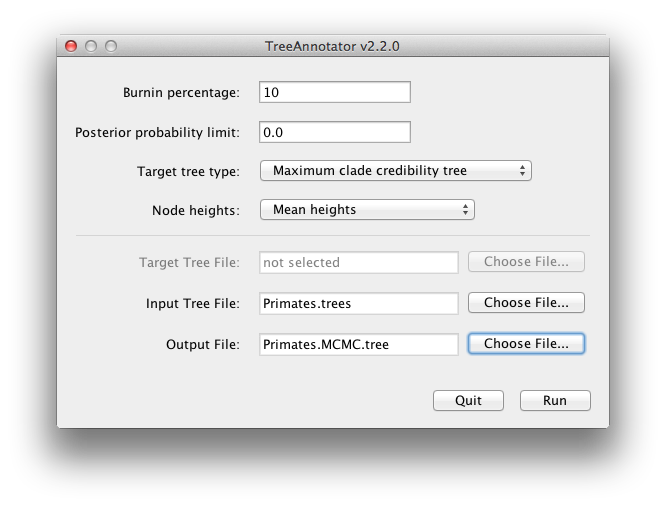
\includegraphics[width=0.8\textwidth]{figures/TreeAnnotator1}
\caption{A screenshot of TreeAnnotator.}
\label{fig:TreeAnnotator1}
\end{figure}

The burnin is the number of trees to remove from the start of the sample. Unlike {\bf Tracer} which specifies the number of
steps as a burnin, in {\bf TreeAnnotator} you need to specify the actual number of trees. For this run, you specified a chain
length of \chainLength{} steps sampling every \logEvery{} steps. Thus the trees file will contain 5000 trees and so to specify a 1\% burnin
use the value 50.

The {\bf Posterior probability limit} option specifies a limit such that if a node is found at less than this frequency in the sample
of trees (i.e., has a posterior probability less than this limit), it will not be annotated. The default of 0.5 means that only nodes
seen in the majority of trees will be annotated. Set this to zero to annotate all nodes.

For {\bf Target tree type} you can either choose a specific tree from a file or ask TreeAnnotator to find a tree in your sample.
The default option, {\bf Maximum clade credibility tree}, finds the tree with the highest product of the posterior probability of
all its nodes.

Choose {\bf Mean heights} for node heights. This sets the heights (ages) of each node in the tree to the mean height across the
entire sample of trees for that clade.

For the input file, select the trees file that BEAST created and select a file for the
output (here we called it \mccTree{}).

Now press Run and wait for the program to finish.

\section{Visualizing the tree estimate}
Finally, we can visualize the tree in another program called {\bf FigTree}. Run this program, and open
the \mccTree{} file by using the Open command in the File menu. The tree should appear.
You can now try selecting some of the options in the control panel on the left. Try selecting
{\bf Node Bars} to get node age error bars. Also turn on {\bf Branch Labels} and select {\bf posterior} to get
it to display the posterior probability for each node. Under {\bf Appearance} you can also tell FigTree
to colour the branches by the rate.
You should end up with something similar to Figure \ref{fig:FigTree}.

\begin{figure}
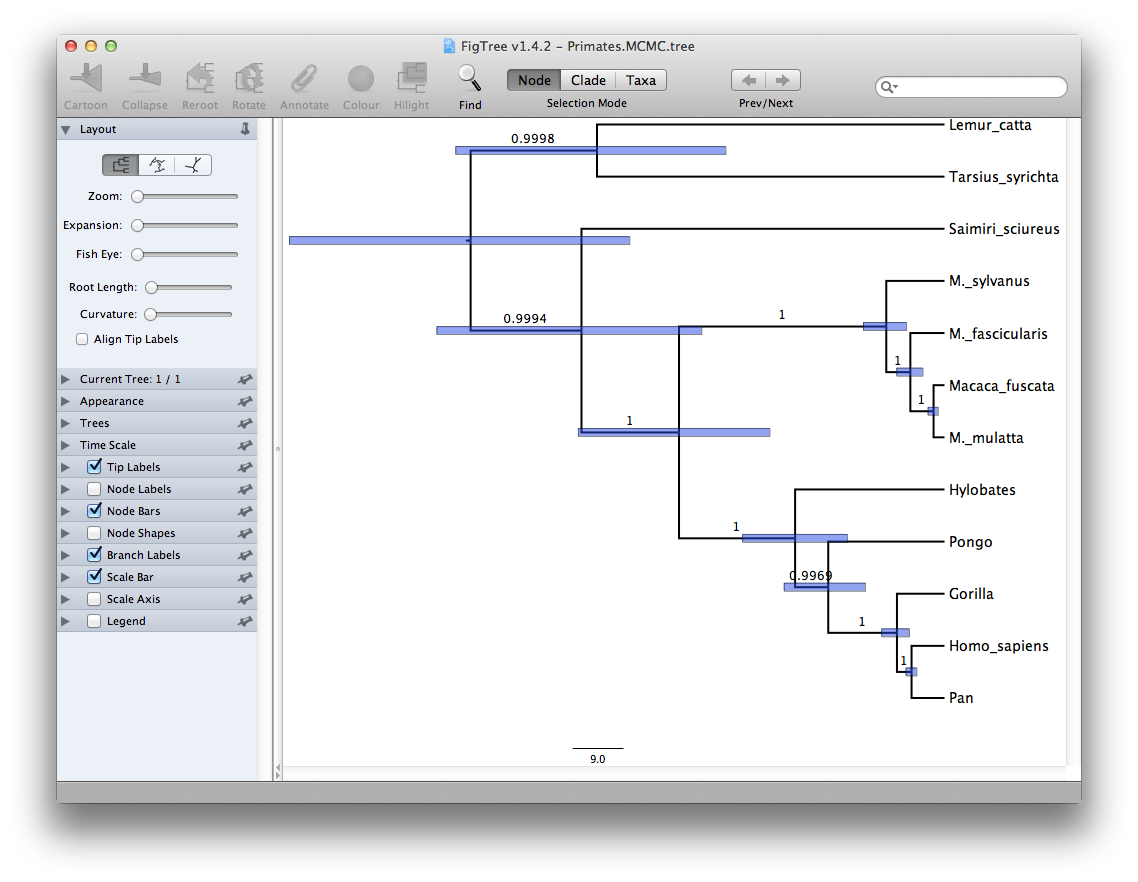
\includegraphics[width=0.8\textwidth]{figures/FigTree}
\caption{A screenshot of FigTree.}
\label{fig:FigTree}
\end{figure}

An alternative view of the tree can be made with DensiTree, which is part of Beast 2. The advantage
of DensiTree is that it is able to visualize both uncertainty in node heights and uncertainty in topology.
For this particular dataset, the dominant topology is present in more than 99\% of the samples. So, 
we conclude that this analysis results in a very high consensus on topology (Figure \ref{fig:DensiTree}).

\begin{figure}
\begin{center}

\includegraphics[width=0.7\textwidth]{figures/DensiTree}
\end{center}
\caption{A screenshot of DensiTree.}
\label{fig:DensiTree}
\end{figure}

\textit{Does the rate of evolution differ substantially amongst different lineages in the tree?}

\vspace{5 mm}
\framebox(420,60){}
\vspace{5 mm}

\section{Comparing your results to the prior}

Using BEAUti, set up the same analysis but under the MCMC options, select the {\bf Sample from prior only} option. This will allow you to visualize the full prior distribution in the absence of your sequence data. Summarize the trees from the full prior
distribution and compare the summary to the posterior summary tree.




% \renewcommand{\refname}{Bibliography}% if you prefer this heading
\bibliographystyle{amsplain} 
\bibliography{DivergenceDatingTutorial}








\newpage
\section*{Notes}

This section has some extra details about aspects of some of the programs.

\subsection*{Guess Dates}

This operation attempts to guess what the dates are from information contained within the taxon names. It works by trying to
find a numerical field within each name. If the taxon names contain more than one numerical field (such as the RSVA
sequences in the MEP tutorial) then you can specify how to find the one that corresponds to the date of sampling. You can either
specify the order that the date field comes (e.g., first, last or various positions in between) or specify a prefix (some
characters that come immediately before the date field in each name). For the RSVA sequences you can select `last' from
the drop-down menu for the order or use the prefix option and specify `\_' (underscore) as the prefix.

In this dialog box, you can also get BEAUti to add a fixed value to each guessed date. In this case the value ``1900'' has
been added to turn the dates from 2 digit years to 4 digit. Any dates in the taxon names given as ``00'' would thus become
``1900''. Some of the sequences in the example file actually have dates after the year 2000 so selecting the will option would
convert them correctly, adding 2000 to any date less than 09. When you press OK the dates will appear in the appropriate
column of the main window. You can then check these and edit them manually as required. At the top of the window you
can set the units that the dates are given in (years, months, days) and whether they are specified relative to a point in the
past (as would be the case for years such as 1984) or backwards in time from the present (as in the case of radiocarbon
ages).

\if0 TODO: update to BEAUti 2
\subsection*{Operators}
Each parameter in the model has one or more ``operators'' (these are variously called moves and proposals by other MCMC
software packages such as MrBayes and LAMARC). The operators specify how the parameters change as the MCMC runs.
The operators tab in BEAUti has a table that lists the parameters, their operators and the tuning settings for these operators.
In the first column are the parameter names. These will be called things like \texttt{kappa} which means the HKY model's
kappa parameter (the transition-transversion bias). The next column has the type of operators that are acting on each
parameter. For example, the scale operator scales the parameter up or down by a proportion, the random walk operator
adds or subtracts an amount to the parameter and the uniform operator simply picks a new value uniformly within a range.
Some parameters relate to the tree or to the divergence times of the nodes of the tree and these have special operators.

The next column, labelled {\bf Tuning}, gives a tuning setting to the operator. Some operators don't have any tuning settings so
have {\bf n/a} under this column. The tuning parameter will determine how large a move each operator will make which will affect
how often that change is accepted by the MCMC which will affect the efficency of the analysis. For most operators (like
random walk and subtree slide operators) a larger tuning parameter means larger moves. However for the scale operator a
tuning parameter value closer to 0.0 means bigger moves. At the top of the window is an option called {\bf Auto Optimize}
which, when selected, will automatically adjust the tuning setting as the MCMC runs to try to achieve maximum efficiency. At
the end of the run a table of the operators, their performance and the final values of these tuning settings will be written to
standard output. These can then be used to set the starting tuning settings in order to minimize the amount of time taken to
reach optimum performance in subsequent runs.

The next column, labelled {\bf Weight}, specifies how often each operator is applied relative to the others. Some parameters
tend to be sampled very efficiently - an example is the kappa parameter - these parameters can have their operators downweighted
so that they are not changed as often (this may mean weighting other operators up since the weights must be
integers).
\fi

\subsection*{Tracer statistics}

The statistics reported in Tracer for each logged quantity are:

\begin{itemize}
\item Mean - The mean value of the samples (excluding the burn-in).
\item Stdev - The standard error of the mean. This takes into account the effective sample size so a small ESS will give a large
standard error.
\item Median - The median value of the samples (excluding the burn-in).
95\% HPD Lower - The lower bound of the highest posterior density (HPD) interval. The HPD is the shortest interval that
contains 95\% of the sampled values.
\item 95\% HPD Upper - The upper bound of the highest posterior density (HPD) interval.
\item Auto-Correlation Time (ACT) - The average number of states in the MCMC chain that two samples have to be separated
by for them to be uncorrelated (i.e. independent samples from the posterior). The ACT is estimated from the samples in the
trace (excluding the burn-in).
\item Effective Sample Size (ESS) - The effective sample size (ESS) is the number of independent samples that the trace is
equivalent to. This is calculated as the chain length (excluding the burn-in) divided by the ACT.
\end{itemize}

\subsection*{TreeAnnotator}

The sampled trees in BEAST are written to a separate file called the `trees' file. This file is a
standard NEXUS format file. As such it can easily be loaded into other software in order to examine the trees it contains. One
possibility is to load the trees into a program such as PAUP* and construct a consensus tree in a similar manner to
summarizing a set of bootstrap trees. In this case, the support values reported for the resolved nodes in the consensus tree
will be the posterior probability of those clades.

TreeAnnotator is a software program distributed with BEAST that can summarize the tree file. 
It takes a single `target' tree and annotates it with the summarized information from the entire sample of trees.
The summarized information includes the average node ages (along with the HPD intervals), the posterior support and the
average rate of evolution on each branch (for models where this can vary). The program calculates these values for each
node or clade observed in the specified `target' tree. The options in TreeAnnotator are detailed below:

\begin{itemize}
\item {\bf Burnin} - This is the number of trees in the input file that should be excluded from the summarization. This value is given
as the number of trees rather than the number of steps in the MCMC chain. Thus for the example above, with a chain of
1,000,000 steps, sampling every 1000 steps, there are 1000 trees in the file. To obtain a 10\% burnin, set this value to
100.
\item {\bf Posterior probability limit} - This is the minimum posterior probability for a node in order for TreeAnnotator to store the
annoted information. The default is 0.5 so only nodes with this posterior probability or greater will have information
summarized (the equivalent to the nodes in a majority-rule consensus tree). Set this value to 0.0 to summarize all nodes in
the target tree.
\item {\bf Target tree type} - This has two options ``Maximum clade credibility'' or ``User target tree''. For the latter option, a
NEXUS tree file can be specified as the Target Tree File, below. For the former option, TreeAnnotator will examine every
tree in the Input Tree File and select the tree that has the highest sum of the posterior probabilities of all its nodes.
\item {\bf Node heights} - This option specifies what node heights (times) should be used for the output tree. If the ``Keep target
heights'' is selected, then the node heights will be the same as the target tree. The other two options give node heights
as an average (Mean or Median) over the sample of trees.
\item {\bf Target Tree File} - If the ``User target tree'' option is selected then you can use ``Choose File...'' to select a NEXUS file
containing the target tree.
\item I{\bf nput Tree File} - Use the ``Choose File...'' button to select an input trees file. This will be the trees file produced by
BEAST.
\item {\bf Output File} - Select a name for the output tree file.
\end{itemize}

Once you have selected all the options, above, press the ``Run'' button. 



\end{document}


